% 4yp.tex -- 4th Year project report
% Max Jaderberg 2012

%-------------------------------
% Preamble
%-------------------------------
\documentclass[11pt, onecolumn, a4paper, final]{report} % 11pt font
\renewcommand{\familydefault}{\sfdefault} % sans-serif (Arial) font
\linespread{2} % double line spacing
\usepackage{amssymb,amsmath}
\usepackage[hang,small]{caption} % makes captions look nicer
\usepackage{subfig}
\usepackage{graphicx}
\usepackage[margin=20mm]{geometry}

% for code listings
\usepackage{listings}
\usepackage{color}
\definecolor{dkgreen}{rgb}{0,0.6,0}
\definecolor{gray}{rgb}{0.5,0.5,0.5}
\definecolor{mauve}{rgb}{0.58,0,0.82}
\lstset{frame=single,
  language=Java,
  aboveskip=3mm,
  belowskip=3mm,
  showstringspaces=false,
  columns=flexible,
  basicstyle={\small\ttfamily},
  numbers=none,
  numberstyle=\tiny\color{gray},
  keywordstyle=\color{blue},
  commentstyle=\color{dkgreen},
  stringstyle=\color{mauve},
  breaklines=true,
  breakatwhitespace=true
  tabsize=3
}

\usepackage{hyperref} % for hyperlinks


\title{The Intelligent Image}
\author{Max Jaderberg\\
	Keble College, University of Oxford}
\date{Trinity Term 2012}


%-------------------------------
% Document
%-------------------------------
\begin{document}

\maketitle

\begin{abstract}

In this report, a large-scale object retrieval system is presented. It allows the user to supply a query image via a web interface, and the web site returns the \emph{intelligent image} -- the objects in the image are automatically labelled and can be clicked for more information.

The system builds upon the state-of-the art in visual object retrieval from large databases -- that is allowing objects to be recognised by searching against millions of images. This notion is explored by using the images contained on the web pages of an online encyclopaedia as the object database. The resulting system can automatically annotate multiple objects within query images, such as the landmarks in a holiday photo. We demonstrated that the system can be implemented with a front end web user interface for interaction. A number of improvements to the base line system are investigated, including a novel method for increasing the matching performance by external database augmentation.

This work is done with the view to scaling up to the database to a corpus of millions of images and objects.

\end{abstract}

\tableofcontents

%-------------------------------
% Introduction
%-------------------------------
\linespread{1}\chapter{Introduction}
\linespread{1}\section{Motivation}
The web contains billions of images, and they are often the focus of attention on the web pages that include them. However, there is almost no information about the content of these images. Images on websites are purely binary data files, occasionally with some associated meta data included in their containing HTML\footnote{Hyper Text Markup Language \url{http://en.wikipedia.org/wiki/HTML}} code. Very little information is available about the images, let alone the objects or scenes contained within them. The aim of this project is to create a system which automatically recognises the objects within images, thus releasing the information within them. This is a large scale object retrieval problem.

Recognising a wide range of objects in an image is not a trivial problem. Objects can be photographed from many different viewpoints, under different lighting conditions, with different cameras, and can be occluded in different ways. This presents problems of robustness to these types of variation and noise. As more objects are added to the database, scaling the solution up becomes a problem. Recognition accuracy drops as there are more objects that could be potential matches, and the matching process gets slower as a larger search is needed. These challenges were addressed throughout the project to ensure a fast, accurate recognition system that can be scaled up to millions of objects.

There are a large number of applications that would benefit from having detailed information on the contents of images. With more knowledge on the objects contained within images, one can create more effective search engines, better cataloguing and classification systems, user interfaces which engage viewers more, and relevant advertising based on the content. Novel applications could also be built, for example, which retrospectively embed geographical information in the image binary by recognising where the image was photographed. The plethora of useful applications provides a great deal of motivation for this project.

\section{The Intelligent Image}

\begin{figure}[t!]
\centering 
\subfloat[]{\label{fig:inta}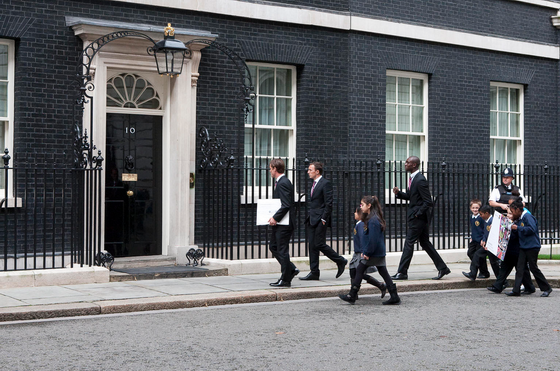
\includegraphics[width=0.4\textwidth]{images/intro1.png}}
\\
\subfloat[]{\label{fig:intb}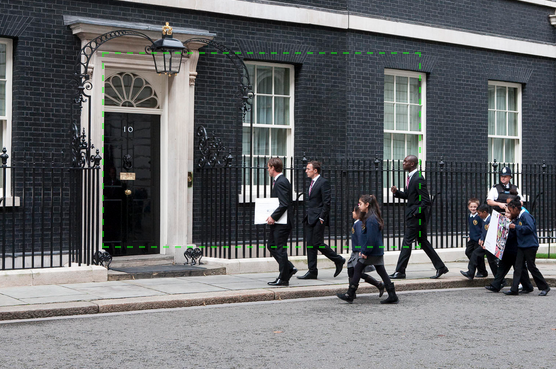
\includegraphics[width=0.4\textwidth]{images/intro2.png}}
~
\subfloat[]{\label{fig:intc}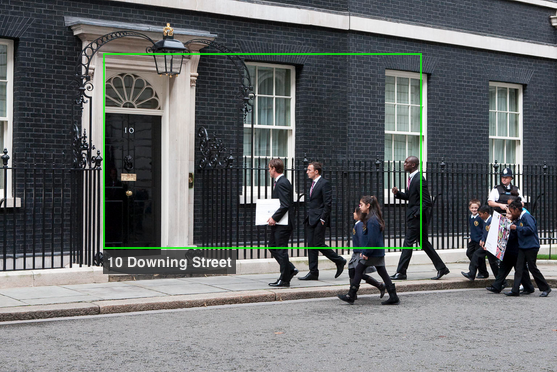
\includegraphics[width=0.4\textwidth]{images/intro3.png}}
\caption{The standard image Figure~\ref{fig:inta} and the intelligent version of the image Figure~\ref{fig:intb} with it's hover over state Figure~\ref{fig:intc}.}
\label{fig:intimage}
\end{figure}

The result of the project is that a query image is inputted, the objects contained within the image are recognised, and the image is returned with the recognised objects \emph{tagged} i.e. the region of the object in the image is outlined and it can be clicked to give relevant information. In this way the standard image has been transformed into the \emph{intelligent image} -- one that knows about the contained scene and can offer up information to the consumer about it's contents.

The tagging process works by matching a section of the query image with an image of an object from a database. The query image is then said to contain this object within the region that matches. To be able to recognise a vast corpus of objects, a large collection of reference images is needed to be available to match against. The database of images of objects is created from Wikipedia \cite{wikipedia} -- a crowd-sourced online encyclopaedia with many images contained within the articles. Each Wikipedia article defines an object, and the images that appear in the article are downloaded to the database. If a query image matches a Wikipedia image in the database, the query image is tagged as the object defined by the article from where the Wikipedia image was downloaded.

The aim of the project is to work towards recognising every object on Wikipedia, however due to time restraints a subset of objects was used for development and testing of the project. The subset of objects chosen are the pages that appear on the Wikipedia page ``List of Structures in London'' \cite{listofstructures}.

\section{Road Map}

The report starts by introducing the background information are previous work published in Chapter~\ref{chpt:background}. This gives a holistic view of the recent innovations in large scale object recognition and retrieval and provides the basis of knowledge used in the project.

Chapter~\ref{chpt:data} gives an in-depth account of the data sources used in the project. This includes the acquisition of the database of Wikipedia images as well as various other datasets used for testing and improving the system.

Chapter~\ref{chpt:system} explains the workings of the baseline system. In this chapter, the steps required for the basic tagging process to work are described. These include the representation of images as collections of \emph{visual words}, the matching of query images to database images by their visual word similarity, and the spatial verification that occurs to confirm a match.

Chapters~\ref{chpt:geoimprovements}~and~\ref{chpt:turboboosting} explain the research and development of improvements to the baseline system to increase object recognition performance. Improvements to the spatial verification stage are made and new feature detectors are implemented. These increase the speed and accuracy of matching. Another novel method was developed to further improve matching performance by augmenting the images in the database with those of an external source.

Finally, Chapter~\ref{chpt:architecture} describes the practical implementation of the object recognition system, as well as the development of a web site to provide a front end user interface to create an intelligent image.


%-------------------------------
% Background
%-------------------------------
\linespread{1}\chapter{Background}
\label{chpt:background}
This project builds upon the vast amount of previous work done on large scale image retrieval and automatic image annotation.

There is no general algorithm to determine whether a query image\footnote{A query image is one that contains a depiction of an object that is to be identified.} contains the same object as an image in a dataset -- the variation in viewpoint, lighting, environment and noise is so large that this task can even be a struggle for humans. However, despite this absence there has been a large amount of work devoted to creating applicable solutions to this problem \cite{quack09,rootsift12,recognitiontree2006,videogoogle2003,philbin2007}. Types of recognition range from scene classification \cite{sceneclass06} to geo-location recognition \cite{knopp10}, however it is specific object annotation that this project aims to achieve.

To be able to query images, a representation of images needs to be computed such that some evaluation of similarity can be applied. All current methods use the notion of detecting salient regions of an image, \emph{features}, and describing them by some vector, a \emph{descriptor}, then using the distance between feature descriptors as a measure of similarity. Basic feature detectors could be corner detectors (such as the Harris detector) and a descriptor could simply be a vector of the local grayscale values, however a method like this is prone to variance due to changes in viewpoints and lighting. It is the work on SIFT descriptors \cite{lowe1999} that is used in this project, as this detector and descriptor is invariant to many of the distortions that occur in images of the same object.

The standard method for image retrieval that is used is the bag-of-words method described in \cite{recognitiontree2006,videogoogle2003}. The approach by Zisserman \emph{et al.} in \cite{videogoogle2003} is closely followed and described fully in Chapter~\ref{chpt:system}. This method involves quantisation of descriptors into ``visual words''\footnote{The term ``words'' in the context of image retrieval will refer to this notion of ``visual words''.} that are used for matching. The paper also describes the influence of work done on web search engines in retrieving useful web pages -- the established methods for document retrieval from text queries described in \cite{searchengines2003,googlearchitecture2003} are adapted for use with visual words. A weighting is applied to each visual words to signify their importance in retrieval (the tf-idf weighting), and inverted file structures are used to provide fast lookup and filtering of the images in the corpus.

Systems such as \cite{philbin2007} have improved recognition performance by making use of the spatial information associated with visual words. Philbin's system performs a re-ranking of the matches based on visual word similarity by estimating an affine transformation between the features in the images of matches and the query image. This ensures that that the objects in a proposed match are structurally similar -- an object in an image is in essence defined not only by the visual words it exhibits, but the positions and scale of those visual words within an object's image. Making use of spatial information was shown to consistently improve performance by 5\%.

Other improvements in image retrieval have come from advancements in clustering methods. Early systems \cite{videogoogle2003} used a flat k-means clustering on feature descriptors to create the visual words, but this is difficult to scale. Cluster hierarchies \cite{hierarchies2006} allow the size of vocabularies to be greatly increased, and \cite{philbin2007} demonstrates that an approximate nearest neighbours method works best. Traditional k-means uses a vast amount of computational power on calculating the nearest neighbours between points and cluster centres, however an approximate method can be used instead by employing a k-d tree and a random forest algorithm \cite{randomforest2005,randomforest1,randomforest2}. The result is that far superior performance can be achieved using very large vocabularies (100K words and greater).

The paper by Quack \emph{et al.} \cite{quack09} describes the application of a state-of-the art system to provide automatic annotation of landmarks in images. A database of images with associated metadata is built by crawling Wikipedia and other internet sources. This is built from the content of a previous paper \cite{quack08}, where photos are mined by geographic proximity from a photo sharing website. The resulting database is clustered into objects, and the images from Wikipedia articles are used for verifying the cluster assignments and provide the labelling. Retrieval is then performed using the bag-of-words approach with spatial verification. Quack \emph{et al.} also use a method of identifying the useful visual words for a cluster of images of objects, allowing the bounding box of the object to be determined as well as facilitating the reduction in the size of the database. However, this system uses the geographical location data associated with photos to allow intelligent clustering and filtering to be done to ensure accurate object representations. This reduces the complexity of the problem compared to the system in this paper where no geographical data is available, but similar performance needs to be achieved.

There are other improvements that have been developed, such as database-side feature augmentation. This method described in \cite{turcot09} is a way of  increasing recognition performance by disseminating the visual word information across the database images. For each image in the database, a query is issued and the spatially verified matches are collected. The visual words of the matches are then augmented with the visual words of the database query image. Further work such as \cite{rootsift12} shows that instead of incorporating the entire vector of visual words from database matches, only the visual words contained within the regions in the database matches that correspond spatially are augmented. 

The state of the art as described in \cite{philbin2007} is used as the basis for this project, with the other research mentioned used for inspiration to enhance the performance.

%-------------------------------
% Data
%-------------------------------
\linespread{1}\chapter{Data}
\label{chpt:data}
There are three main datasets used by the application:

\begin{itemize}
\item The images from Wikipedia used to build the database of objects (Section~\ref{sec:modelimages}). These are referred to as \emph{model images} and are used in Chapter~\ref{chpt:system} when creating the baseline system.

\item The images from Microsoft Bing that are used for the augmentation improvements. A description of this dataset is found in Section~\ref{sec:turboimages}, and their usage is in Chapter~\ref{chpt:turboboosting}.

\item Test images gathered from Google Images, described in Section~\ref{sec:validationimages} and used in Section~\ref{sub:performance}.
\end{itemize}

Table~\ref{tbl:data} gives an overview of the data used. All images that are used are resized so that their larger dimension does not exceed 1000 pixels to reduce storage space and provide homogeneity. This chapter describes the various datasets and how they are acquired. 

\begin{table}[hbtp]
\begin{center}
\begin{tabular}{c|c|c|c|}
\cline{2-4}
 & Source &  \# Images &  \# Classes \\ 
 \cline{1-4}
\multicolumn{1}{|c|}{Model images} & Wikipedia & \texttt{3963} & \texttt{732} \\  
\cline{1-4}
\multicolumn{1}{|c|}{Augmentation images} & Microsoft Bing & \texttt{18273} & \texttt{732} \\  
\cline{1-4}
\multicolumn{1}{|c|}{Test images} & Google &  \texttt{701} & \texttt{294} \\  
\cline{1-4}
\end{tabular}
\end{center}
\caption{A summary of the datasets.}
\label{tbl:data}
\end{table}

\section{Model Images}
\label{sec:modelimages}
The model comprises of a dataset of images that depict the objects that are to be able to be recognised. As explained fully in Chapter~\ref{chpt:system}, an object is recognised by matching a sub-part of the query image containing an object to an image of the object stored in a database. This database of images of objects is created from the images from Wikipedia, and the images downloaded from Wikipedia for this database are known as \emph{model images}.

Each page of Wikipedia that contains images represents an object which can be matched. The database of images which is used to build the model is simply created by visiting each page on Wikipedia for the objects desired and downloading the relevant images contained on the web page, labelling those images as being associated with the object. A script automates this process of building the model database.

The subset of Wikipedia articles used in this project are the articles containing images linked to by the ``List of Structures in London'' page \cite{listofstructures}. This results in 732 unique objects for the database comprising of 3923 images (on average 6 images per class). The images are pulled directly from the articles for the objects. \cite{listofstructurespdf} is a list of all the classes used in the application.

Figure~\ref{fig:classes} illustrates some of the object classes and the model images downloaded for them.

\begin{figure}[!h]
\centering
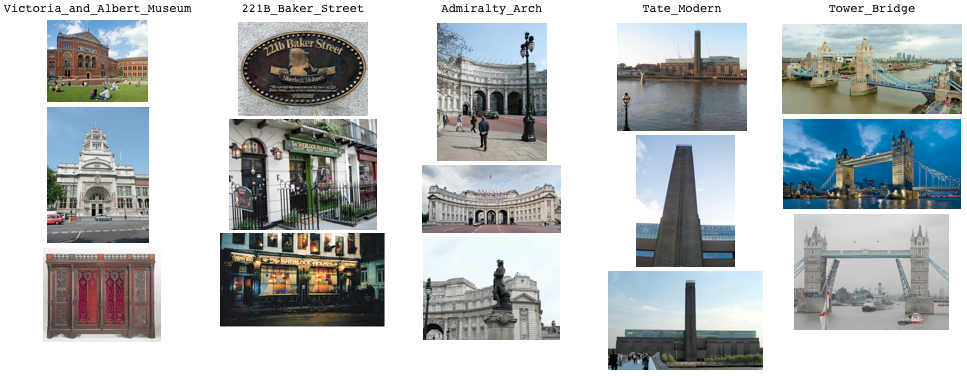
\includegraphics[width=0.95\textwidth]{images/modelimages.png}
\caption{A selection of some object classes with the model images associated with them.}
\label{fig:classes}
\end{figure}

\subsection{Data Acquisition}

To automate the downloading of object images from Wikipedia, Python\footnote{\url{http://www.python.org}} is used. Wikipedia offers a public application programming interface (API) over HTTP to access its data, as it is built on the MediaWiki framework\footnote{The MediaWiki framework was originally developed for Wikipedia and provides an API over HTTP as standard. \url{http://www.mediawiki.org/wiki/API} provides documentation for the API.}. However it is cumbersome and not easy to consume. Instead, a web crawler was written to explore Wikipedia pages and extract the relevant images. 

\begin{figure}[htb]
\centering 
\subfloat[]{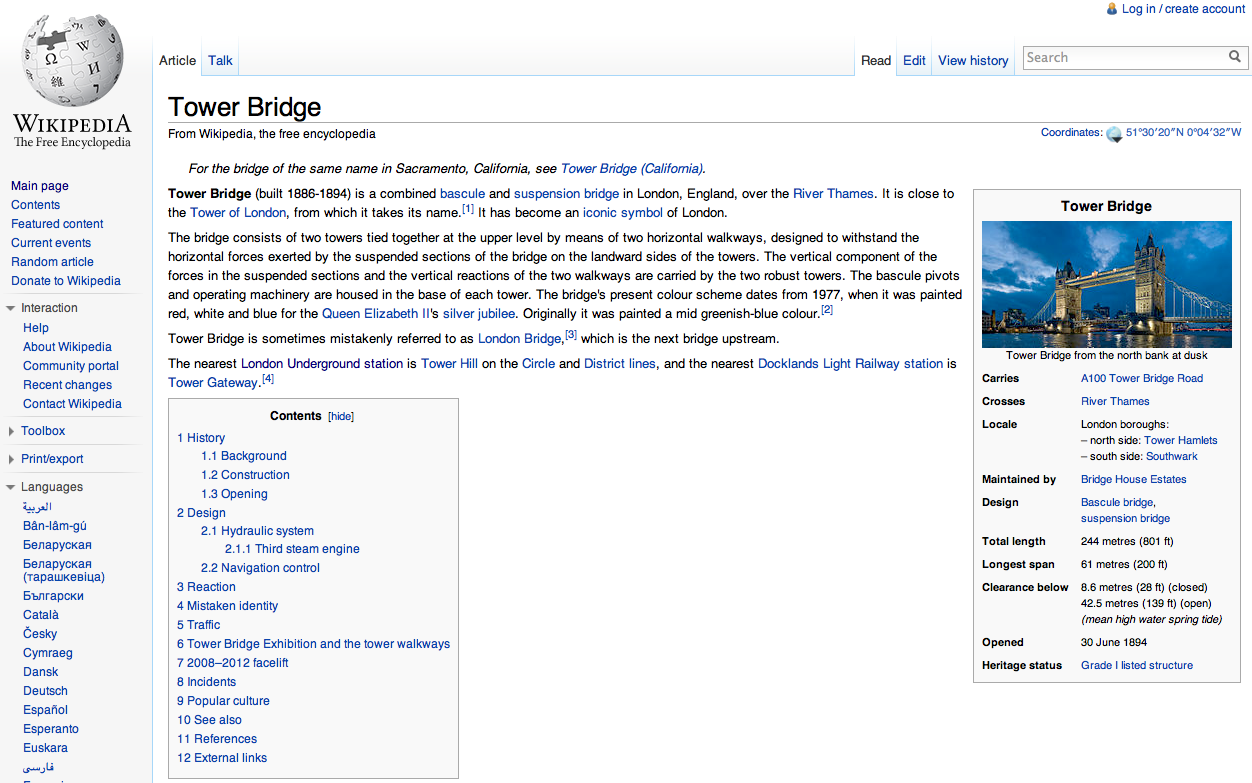
\includegraphics[width=0.5\textwidth]{images/wikipedia-article1.png}}
\subfloat[]{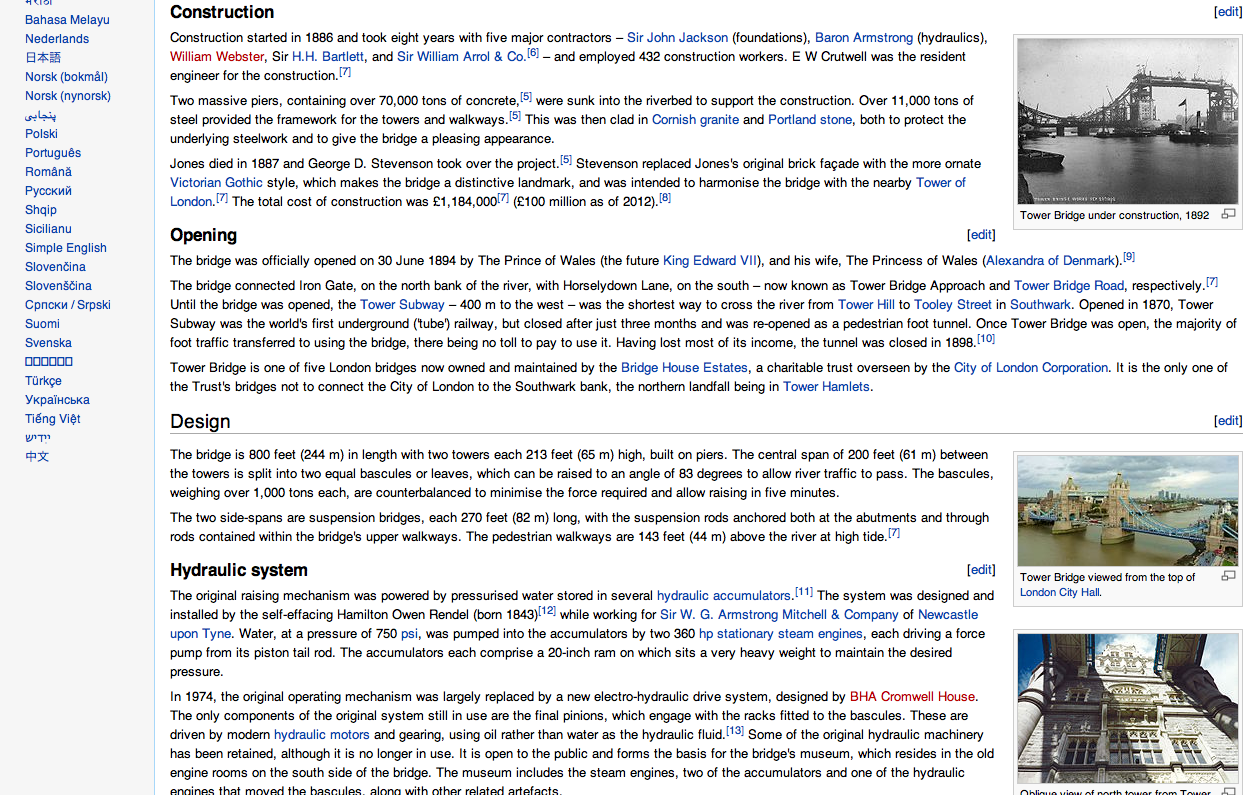
\includegraphics[width=0.5\textwidth]{images/wikipedia-article2.png}}
\caption{The Wikipedia page for ``Tower Bridge''. Note the images contained are those used in the model to represent this object.}
\label{fig:wikipage}
\end{figure}

A crawler object in Python finds all the images and notes the URLs of them for subsequent download. Firstly, the HTML of the Wikipedia page must be downloaded, as it appears to a web browser. However, Wikipedia does not allow crawlers and automated bots to access its web pages. To overcome this, the HTTP header\footnote{\url{http://www.w3.org/Protocols/rfc2616/rfc2616.html} describes the Hyper Text Transport Protocol and the various header fields.} of the crawler is edited to emulate that of a browser. This is implemented using the urllib2 library\footnote{\url{http://docs.python.org/library/urllib2.html}}. The HTML document for each Wikipedia page is parsed using the BeautifulSoup library\footnote{\url{http://www.crummy.com/software/BeautifulSoup/}}. All the anchor elements are found and stored for further crawling. The images contained within the HTML are also found by looking within the part of the HTML document that is unique to the specific Wikipedia page.

The output of the crawler is a CSV file of the image URLs and the object class the images belong to. The object class is simply named from the URL of the Wikipedia page (for example all images appearing on \url{http://en.wikipedia.org/wiki/Tower_Bridge} will have class \lstinline!Tower_Bridge!).

The images mentioned in the CSV file produced by the crawler are then downloaded to local storage. Each image that appears on Wikipedia has a ``file page'' which displays the image along with properties and metadata on the image\footnote{For an example see \url{http://en.wikipedia.org/wiki/File:Tower_bridge_London_Twilight_-_November_2006.jpg}}. This ``file page'' is visited for each image, and the page is parsed to extract the storage URL of the image as well as its file format and original size. As the application resizes all images that exceed 1000 pixels to 1000 pixels, it is a waste of time and storage space to download the original image and later resize it. Instead, Wikipedia's inbuilt thumbnail engine is exploited, which resizes the image on Wikipedia's servers and allows you to download a thumbnail of a user selected width\footnote{\url{http://www.algorithm.co.il/blogs/programming/wikipedia-images/} describes how this is exploited}. Therefore if the original image on Wikipedia exceeds 1000 pixels, the 1000 pixel thumbnail version is downloaded instead. The images downloaded are saved in a folder named after it's class. The result is a directory containing a folder for each class, within which are the images for that class.


\section{Augmentation Images}
\label{sec:turboimages}
One of the methods of improving the performance of the baseline system is by augmenting the model images with the data from an external source of images. This process, described in Chapter~\ref{chpt:turboboosting}, requires a dataset of images to use for augmentation. This is the focus of this section.

To achieve effective augmentation, many additional images are needed to supplement the model images acquired from Wikipedia. Microsoft Bing is used as the source of the augmentation images. For each class, 25 additional images are downloaded to boost that class.

Overall, the dataset contains 18273 images distributed over the 732 object classes. A selection of the augmentation images dataset is shown in Figure~\ref{fig:augimages}.

\begin{figure}[t]
\centering
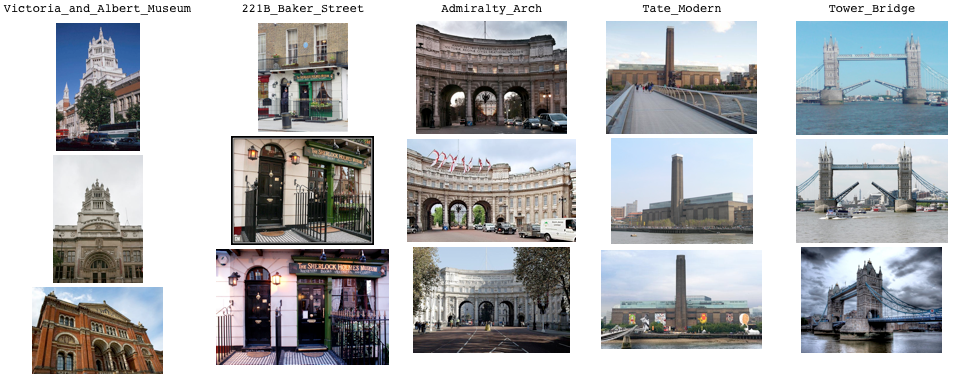
\includegraphics[width=0.95\textwidth]{images/augmentationimages.png}
\caption{A selection of the augmentation images for some object classes.}
\label{fig:augimages}
\end{figure}

\subsection{Data Acquisition}

Bing offers a public API that can be used to perform image searches programmatically. After obtaining an application ID from Bing for authentication, complex search requests can be made over HTTP, with the results returned in JavaScript Object Notation (JSON) format\footnote{JSON is an alternative to XML for representing structured data. \url{http://www.json.org/} provides more information.}.

Bing image search takes a number of keywords -- the query -- and returns a list of images from web pages related to the query. Filters can be applied to further narrow down the search to the most relevant images. This is shown in Figure~\ref{fig:bingimages} on the website version of Bing. The ``Style'' and ``Size'' filters are especially useful in this application, as all images should be photographs for the List of Structures in London dataset, and large images are preferable so as to include as much detail as possible. Setting these filters precludes many instances of graphics and logos which are not suitable for augmentation.

\begin{figure}[t!]
\centering 
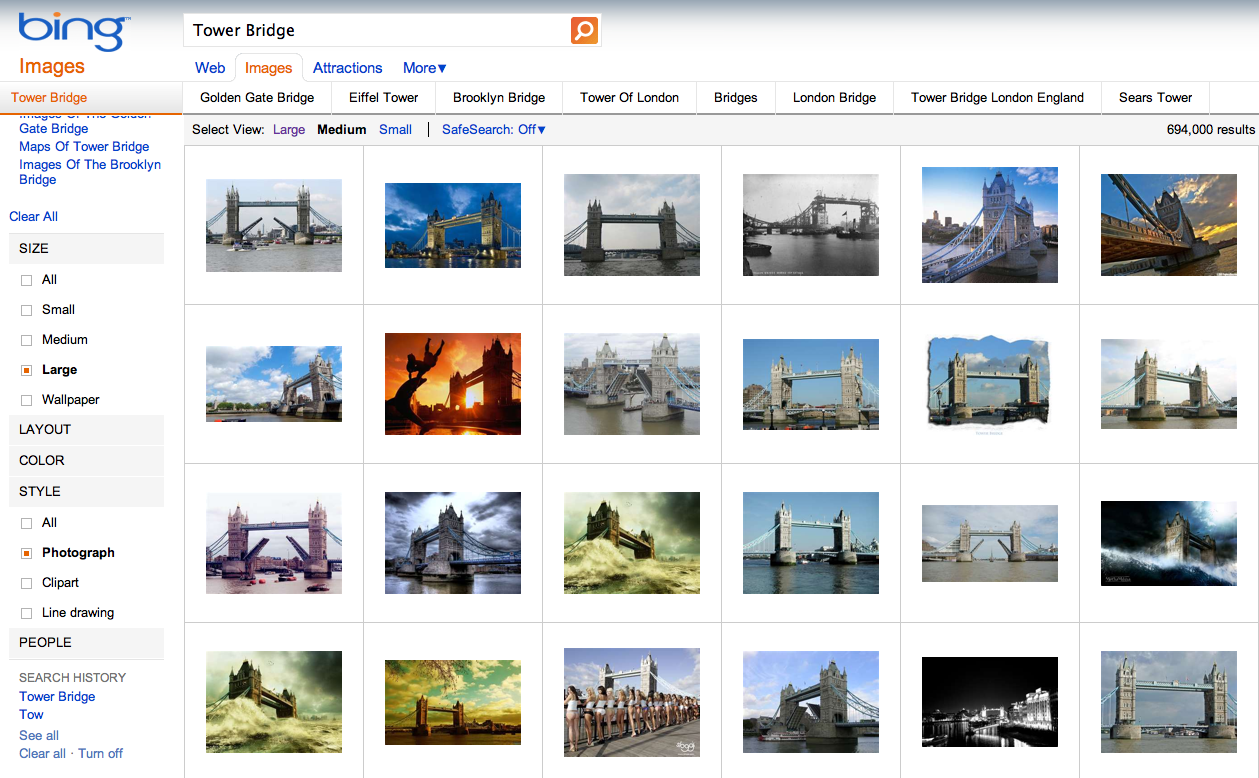
\includegraphics[width=0.9\textwidth]{images/bing-images.png}
\caption{The browser interface of Bing image search which is replicated in the API query URL. Note the filters in the left column.}
\label{fig:bingimages}
\end{figure}

All the parameters that appear in the web interface for Bing image search can be replicated in the API request with query parameters. A MATLAB script is used to consume the API and download the images. Listing~\ref{lst:bingapi} shows the URL used for the API call to get the search results for the images for a particular class. The URL encoded\footnote{URL encoding ensures that all characters are in a form which can be used as a URL. See \url{http://www.w3schools.com/tags/ref_urlencode.asp} for more information.} class name is used as the query. For example, for the class \lstinline!Tower_Bridge!, the variable \lstinline!search_term! appearing in Listing~\ref{lst:bingapi} will be set to \lstinline!"Tower%20Bridge"! (note \lstinline{" "} is URL encoded as \lstinline{"%20"}). Both the ``Style'' and ``Size'' image filters are set to ``Photo'' and ``Large'' respectively by setting the \lstinline!Image.Filters! parameter.

\linespread{1} % single line spacing
\lstset{language=Matlab,caption=A Bing image search API request.,label=lst:bingapi}
\begin{lstlisting}[frame=single]
%% MATLAB
request_url = ['http://api.bing.net/json.aspx?' ...
                   'AppId=' app_id ...
                   '&Query=' search_term ...
                   '&Sources=Image' ...
                   '&Version=2.0' ...
                   '&Adult=Strict' ...
                   '&Image.Count=' nPhotos ...
                   '&Image.Filters=Style:Photo+Size:Large' ...
                   '&JsonType=raw' ...
                  ];
% Read the result of the request
response = urlread(request_url);
% Parse the result from JSON to MATLAB structure form
resp_struct = parse_json(response);
\end{lstlisting}
\linespread{2} % double line spacing

Using MATLAB's inbuilt \lstinline!urlread! function, the search results are requested and returned in JSON format. The JSON result is then parsed and converted into a MATLAB structure object for reading. Each element in the array \lstinline!Results! is an image result. Each image is then downloaded from its \lstinline!MediaUrl! field using a modified version of the \lstinline!imread! function which allows for request timeouts, as some image resources may have expired since their submission to the Bing database.

The downloaded images are resized if larger than 1000 pixels and stored in a folder named after its class. As with the model images, the result is a directory containing a folder for each class, within which are the augmentation images for that class.

\section{Test Images}
\label{sec:validationimages}

Images are needed to test and quantify the yield performance of the object recognition system (see Subsection~\ref{sub:performance}). Therefore a separate dataset of images with their ground-truth classes is needed. Ideally all classes would be tested and each test image should be a fair representation of the object of that class.

Google image search is used first to automatically download 8 images for each class. However, many of the automatically downloaded test images are inaccurate representations of the object in question, or are completely unrelated due to a generic search term giving results that do not even show the object. For example, a search for the object ``Foyles'' (a book shop in London), gives some representative images of the shopfront, but there are also many images of logos, books, people and the inside of the store. As what is being tested is whether the \emph{structure} of Foyles book shop can be recognised, these other images should be discarded. Another example is the search for ``55 Broadway'' gives some images of the building 55 Broadway in New York City, rather than London. Therefore, after automatic download, the dataset is manually refined to remove unrepresentative images.

The resulting test images dataset totals 701 images, spread out over 294 object classes. The distribution of test images is shown in Figure~\ref{fig:testimageshist} which shows the histogram of how many classes contain a number of test images. Some examples of test images are shown in Figure~\ref{fig:validationimages}. 

\begin{figure}[t!]
\centering
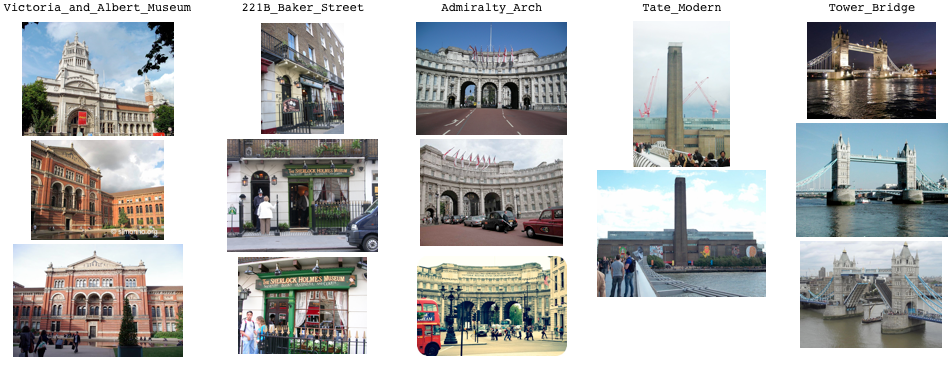
\includegraphics[width=0.95\textwidth]{images/validationimages.png}
\caption{A selection of some of the test images for objects.}
\label{fig:validationimages}
\end{figure}

\begin{figure}[t!]
\centering
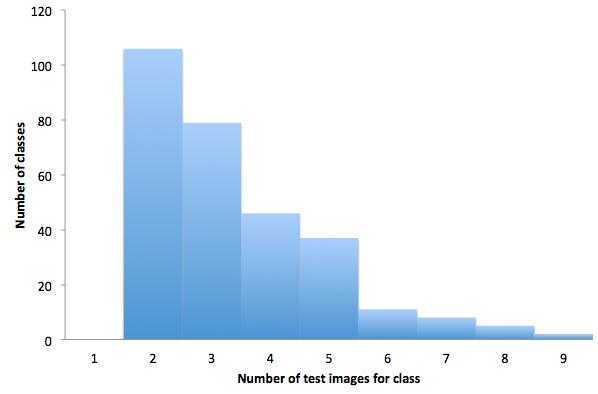
\includegraphics[width=0.6\textwidth]{images/testimageshist.png}
\caption{A histogram of the number of test images per class.}
\label{fig:testimageshist}
\end{figure}

\subsection{Data Acquisition}

Google image search is very similar to Bing image search described in the previous section. However the results are markedly different, providing another set of images that are perfect for testing. Google offers an API over HTTP that can be used to search based on a text query and, as with Bing, filters can be applied. The result is returned in JSON format.

\linespread{1} % single line spacing
\lstset{language=Matlab,caption=A Google image search API request.,label=lst:googleapi}
\begin{lstlisting}[frame=single]
%% MATLAB
request_url = ['https://ajax.googleapis.com/ajax/services/search/images?v=1.0' ...
	'&q=' search_term ...
	'&as_filetype=jpg' ...
	'&imgsz=xxlarge' ...
	'&imgtype=photo' ...
	'&rsz=8' ...
];
% Read the result of the request
response = urlread(request_url);
% Parse the result from JSON to MATLAB structure form
resp_struct = parse_json(response);
\end{lstlisting}
\linespread{2} % double line spacing

Listing~\ref{lst:googleapi} shows the formulation and request of a Google search API request. As with the Bing requests, the search term is the URL encoded class name. The JSON response is parsed into a MATLAB object and the \lstinline!url! field is used to download the image.

As with the augmentation images, the downloaded Google images are resized if larger than 1000 pixels and stored in a folder named after its class. Again, the result is a directory containing a folder for each class, within which are the test images for that class.

After automatic download of potential test images for each class, the dataset was checked over manually. Images that appear in the model dataset, as well as images that do not fairly depict the class they are to test are removed from the test set. 

\subsection{Performance Measure}
\label{sub:performance}

The test images are used to measure the performance of the system. A query is issued for every test image and the label assigned by the system is compared to the ground-truth object label of the test image. The performance is measured simply as the ratio of test images that are correctly labelled by the system, to the total number of test images, expressed as a percentage. This is defined as the \emph{yield}, and is described by 
\begin{equation}
yield = \frac{1}{N}\sum_{i=1}^{N} [y_i=f(x_i)]
\label{eqn:yield}
\end{equation}
where $y_i$ is the ground-truth class of image $x_i$, $f(x_i)$ is the class given by the system, and $N$ is the total number of test images (701 in this case). For example, a yield of 30\% means that 210 of the 701 test images were annotated correctly. It should be noted that each test image is only associated with one ground-truth class\footnote{This means to say that a test image cannot contain multiple objects. There is however a problem during testing of some test images being matched accurately with model images, but their classes being different due to the labelling process. For example, a test image of Big Ben may be labelled as Houses of Parliament -- this would be recorded as a false positive label, even though this would be a perfectly acceptable label for the test image. The result is some false positive labelling which is not actually incorrect. Therefore the true yield performances are always slightly higher than given due to some incorrect false positive labelling during testing.}.

With this measure of performance, the performance of the baseline system (Chapter~\ref{chpt:system}) can be quantified, and the effects of the improvements described in Chapter~\ref{chpt:geoimprovements} and Chapter~\ref{chpt:turboboosting} can inpterpreted.


%-------------------------------
% Baseline system
%-------------------------------
\linespread{1}\chapter{Baseline system}
\label{chpt:system}
The baseline system draws upon the research and literature mentioned in Chapter~\ref{chpt:background}. Upon starting the project, an application was provided written in MATLAB and C. However it simply ranked the similarity of database images to a query image, and the database was one of structures in Oxford that has been well researched. There was therefore a very large amount of work to take the starter application forward to the full system proposed by this project.

There are two separate processes forming the project. The first is the pre-computation process that creates the databases and data structures required for object recognition. The second is the object recognition process that takes a query image and returns the names and locations of the objects in the image. A summary of these two processes is described in Figure~\ref{fig:precompprocess} and Figure~\ref{fig:searchprocess} respectively.

\begin{figure}[htb]
\centering 
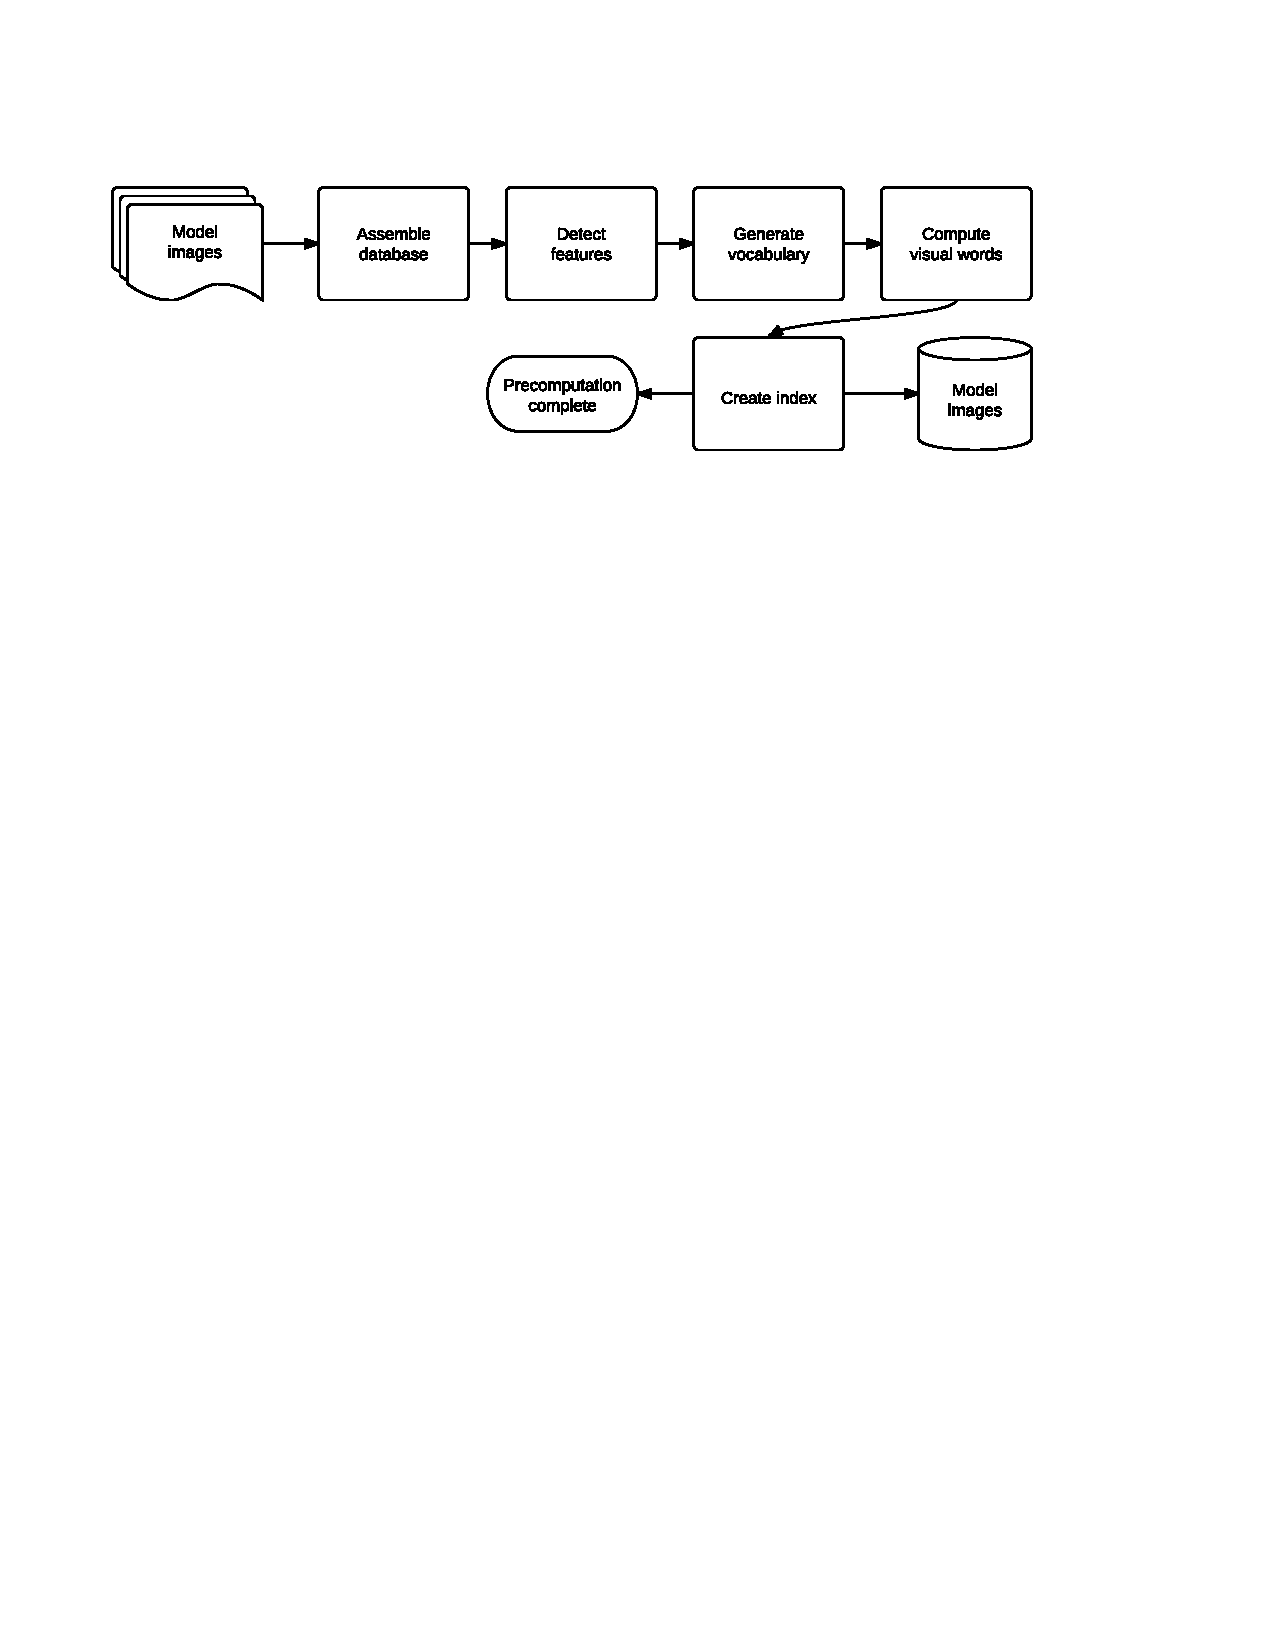
\includegraphics[width=0.9\textwidth]{images/PrecomputeProcess.pdf}
\caption{The flow diagram for the basic pre-computation process.}
\label{fig:precompprocess}
\end{figure}

\begin{figure}[htb]
\centering 
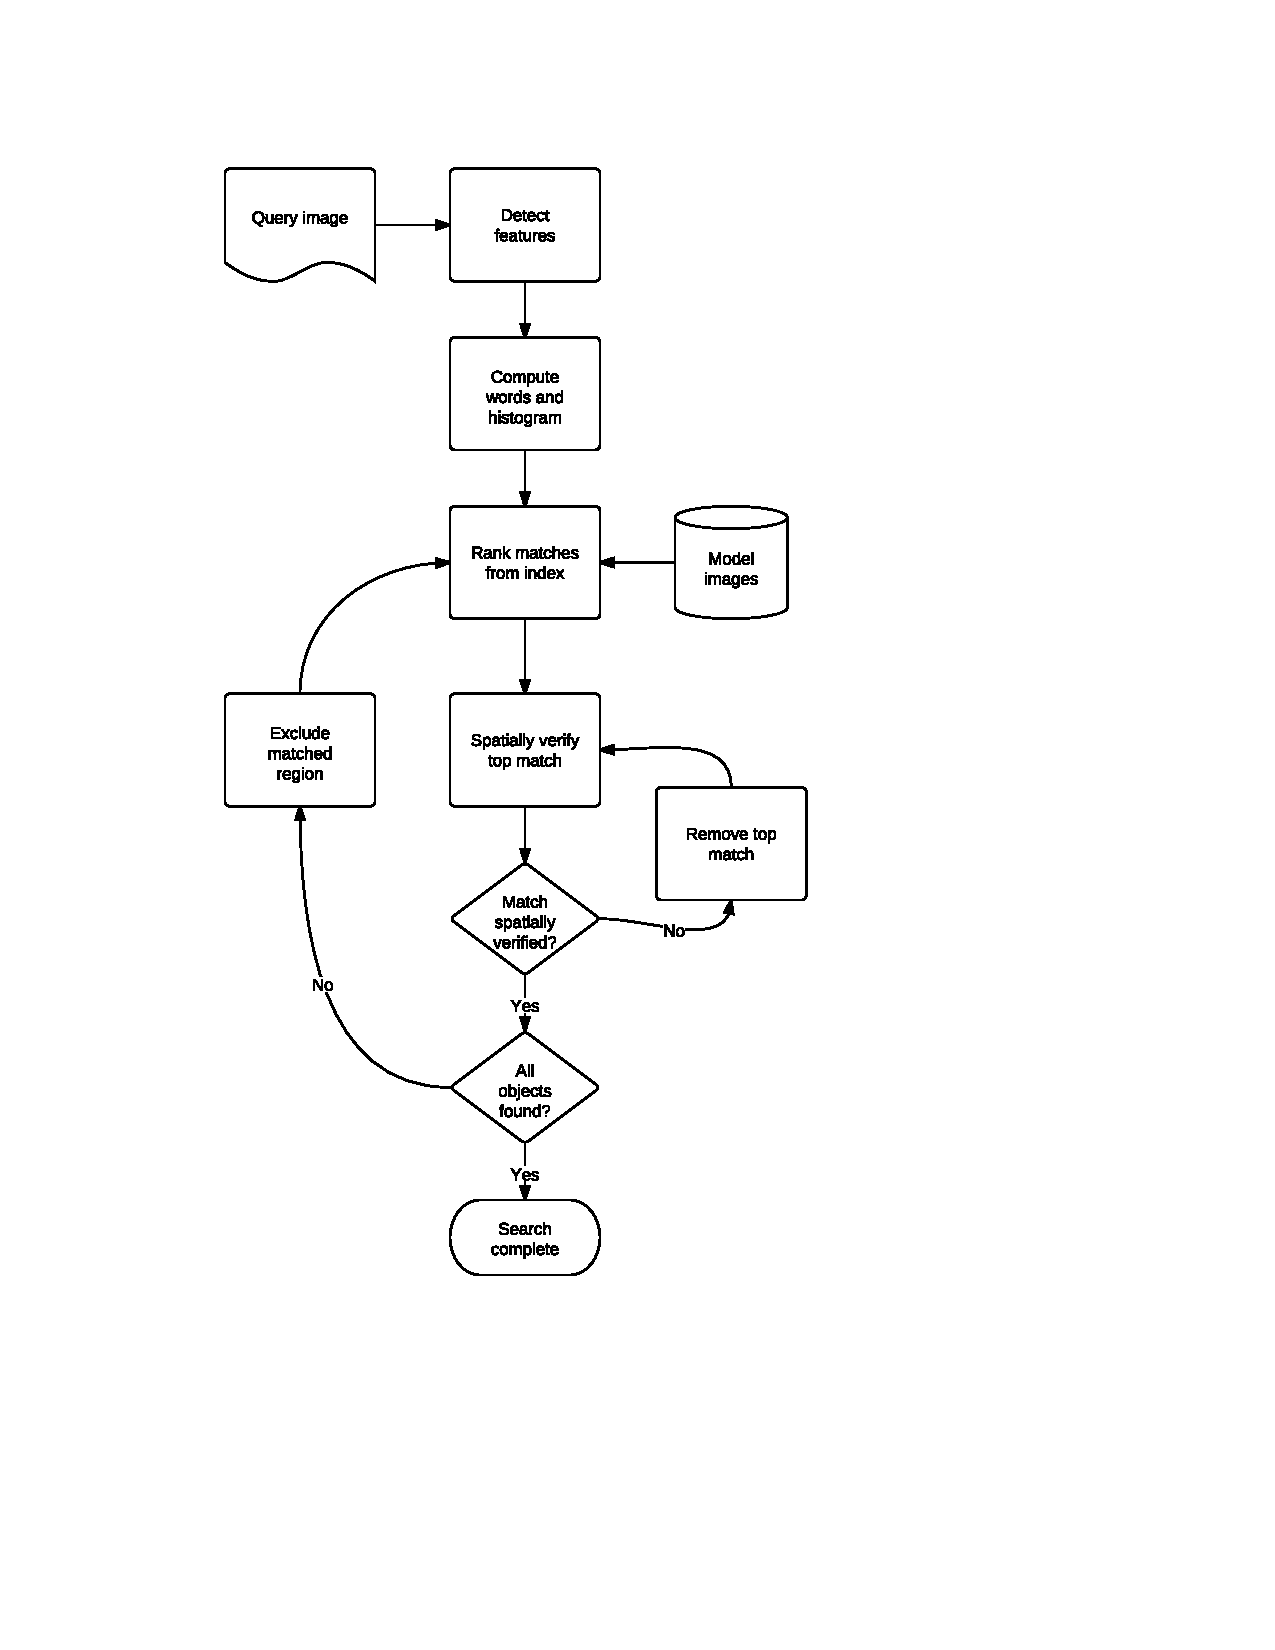
\includegraphics[width=0.9\textwidth]{images/SearchProcess.pdf}
\caption{The flow diagram for the basic object recognition process.}
\label{fig:searchprocess}
\end{figure}

The pre-computation process is run once on the dataset to produce the database and working data structures required for the object recognition process. For each model image, the features are detected and associated descriptors generated. This is described further in Section~\ref{sec:featuredetection}. A sample of the features are then used to generate the visual word vocabulary (Section~\ref{sec:visualwords}). The histograms of visual words are then weighted and collected into an index ready for querying (Section~\ref{sec:histograms}). This completes the basic pre-computation process and the system is ready for use.

The object recognition process takes a query image and attempts to recognise the objects contained within the image. Firstly, the feature descriptors are computed for the detected features within the query image. The visual words are computed based on the vocabulary created during the pre-computation process, and the weighted histogram produced for the query image. A search is then performed on the index of histograms for the model images (see Section~\ref{sec:histograms}) the output of which is a list of images based on how highly they match the query image. Going down the list of top matches by histogram, spatial verification is performed to ensure the visual words in both the query image and match image form the same shaped object (all objects are assumed rigid). This is described in Section~\ref{sec:spatialverification}. Once a match has been spatially verified, this object is deemed recognised and added to the list of found objects. Multiple matching is then performed by repeating this process, excluding regions of the image containing a previously recognised object (Section~\ref{sec:multiobject}).

The remainder of this chapter describes further details of the parts of the processes described above.

\section{Feature Detection and Description}
\label{sec:featuredetection}
The feature detection and description methods used are the original scale-invariant feature transform (SIFT) algorithms. The advantages of using SIFT are that the detected features and their descriptors are invariant to image translation, scaling, and rotation, partially invariant to illumination changes and robust to local geometric distortion. This is essential to be able to match the same object features across varied sources of images.

The SIFT features are defined as maxima and minima of the result of difference of Gaussians function\footnote{\url{http://en.wikipedia.org/wiki/Difference_of_Gaussians}} applied in scale-space to a series of smoothed and resampled images. Low contrast candidate points and edge response points along an edge are discarded. These features are then described by the SIFT feature descriptor -- a 128-dimensional vector.

The result of the SIFT feature detection and description algorithm are two matrices. The first is a matrix of feature points or frames, 
\begin{equation}
\left[ \begin{array}{ccccc}
x_1 & x_2 & \cdots & x_{N-1} & x_N \\
y_1 & y_2 & \cdots & y_{N-1} & y_N \\
s_1 & s_2 & \cdots & s_{N-1} & s_N \\
\theta_1 & \theta_2 & \cdots & \theta_{N-1} & \theta_N
\end{array}\right]
\label{eqn:frames}
\end{equation}
where each column describes the position $(x_i, y_i)$ in the image, the scale $s_i$ and orientation $\theta_i$ for feature $i$. Corresponding to the frames matrix is a descriptor matrix, where each column is the 128-D vector $\mathbf{d_i}$ that describes feature $i$:
\begin{equation}
\left[ \begin{array}{ccccc}
\mathbf{d_1} & \mathbf{d_2} & \cdots & \mathbf{d_{N-1}} & \mathbf{d_N} 
\end{array}\right].
\label{eqn:descrs}
\end{equation}

\section{Visual Words}
\label{sec:visualwords}
To avoid matching features in unbounded, 128-dimensional space, the SIFT features are quantised. These quantised SIFT features are known as visual words.

During the pre-computation process, the vocabulary of words is created. The vocabulary is essentially the clustering of SIFT space. The number of clusters (visual words) to be created is the vocabulary size, 100K for this application. Vocabulary creation is done using the approximate nearest neighbours K-means algorithm. The clustering is performed on a random sample from all the feature descriptors for the entire model images dataset. The number of features sampled was 30 times the size of the vocabulary, i.e. 3 million. 

The result of the vocabulary creation is a kd-tree which can be used to get the word associated with a SIFT descriptor. Each word is assigned an ID, and the images can then be represented as a list of words, where each word is the nearest visual word to the SIFT descriptor.

\section{Histograms and Index}
\label{sec:histograms}
The images are represented by a list of words as described in the previous section. This list of words can in turn be represented as a histogram, with each element containing the number of occurrences in the image of the word with ID equal to the element number. Therefore each histogram is a sparse 100K element array. Two examples of the raw histograms are shown in Figure~\ref{fig:rawhist1} and Figure~\ref{fig:rawhist2}.

The term frequency-inverse document frequency\footnote{This is a practice developed originally for text search. See \url{http://en.wikipedia.org/wiki/Tf*idf} for more information.} (tf-idf) weights are then computed for each word across the entire dataset of model images. These weights are applied to the histograms to down-weight common, uninformative visual words and up-weight unique, informative visual words. The differences in histograms before and after weighting are illustrated in Figure~\ref{fig:histograms}.

\begin{figure}[htb]
\centering 
\subfloat[Tower Bridge image 1]{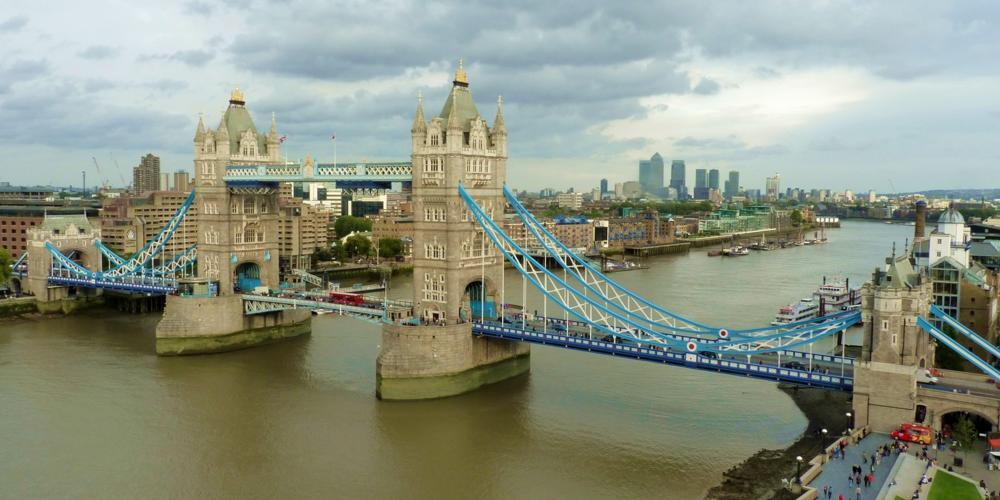
\includegraphics[width=0.3\textwidth]{images/tb_city_hall.jpg}}
~
\subfloat[Raw histogram for image 1]{\label{fig:rawhist1}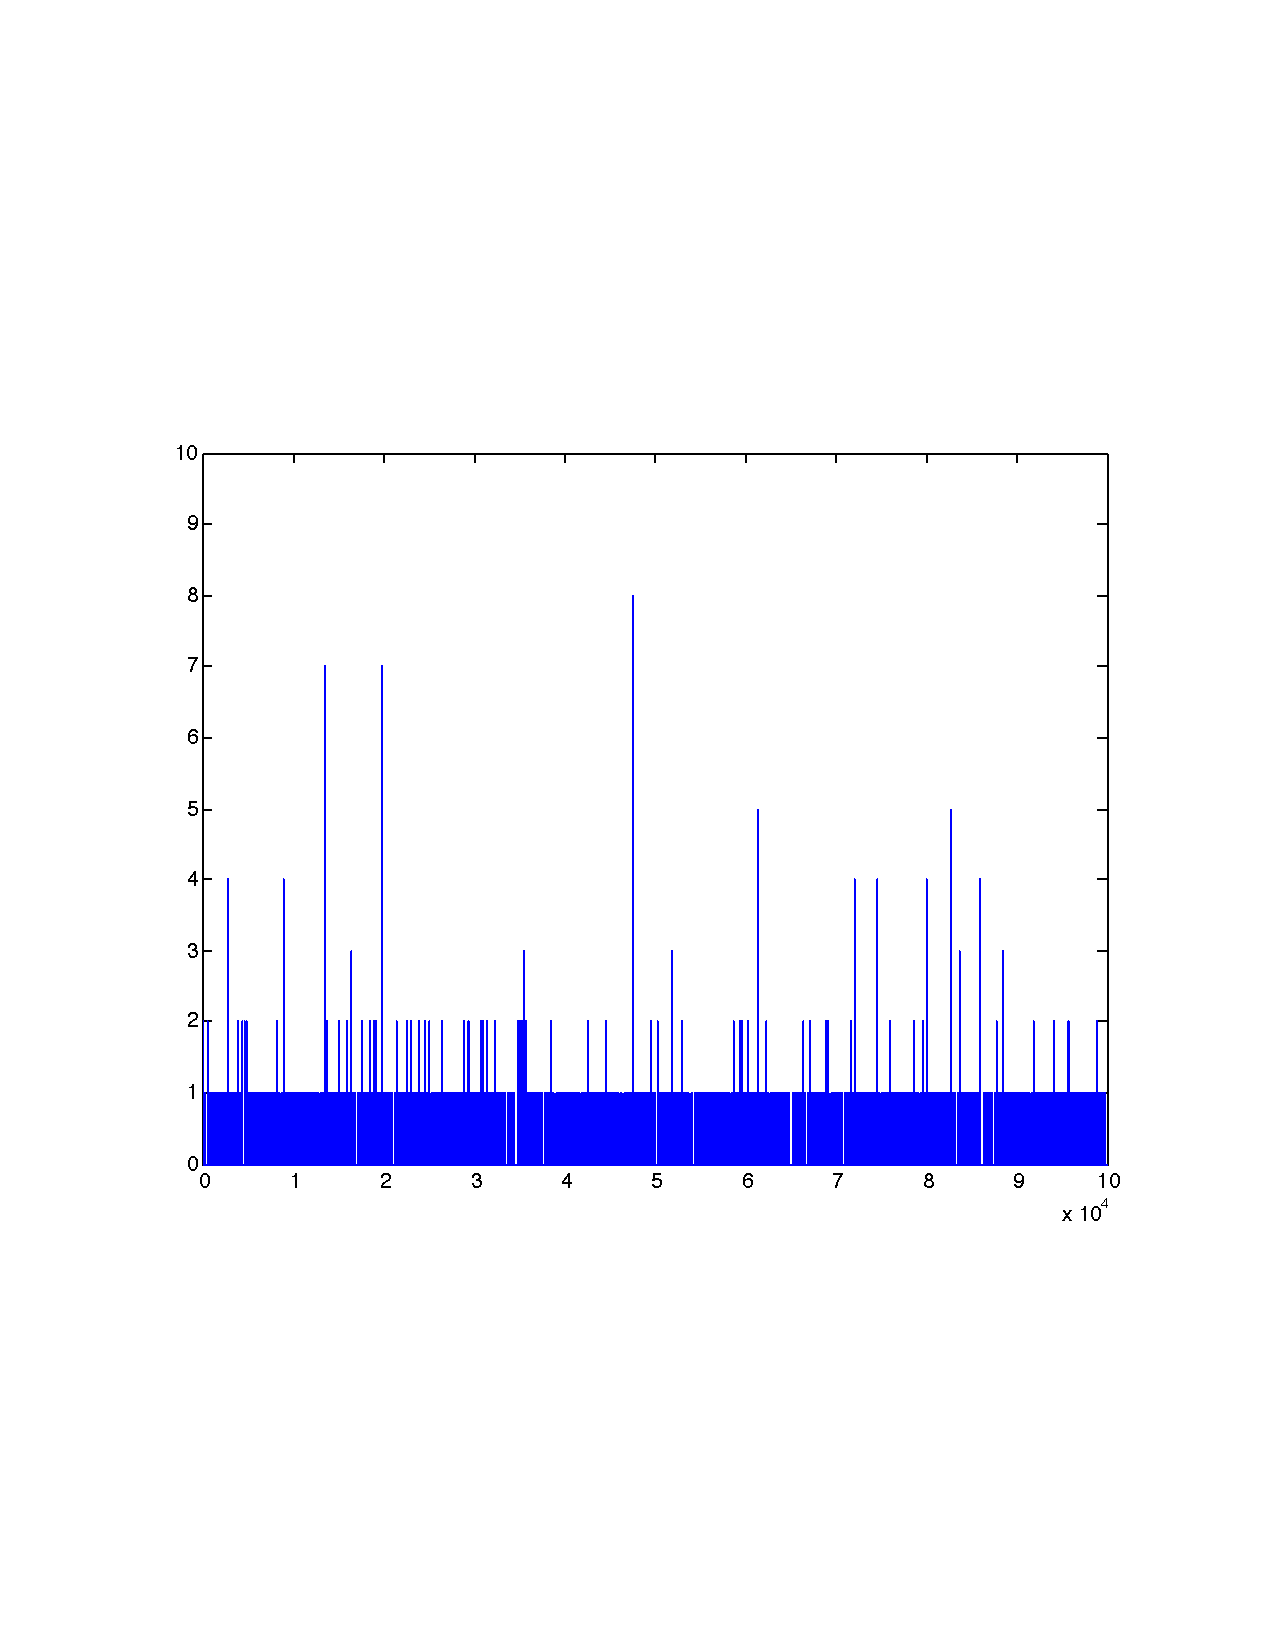
\includegraphics[width=0.3\textwidth]{images/tb_city_hall.pdf}}
~
\subfloat[Weighted histogram for image 1]{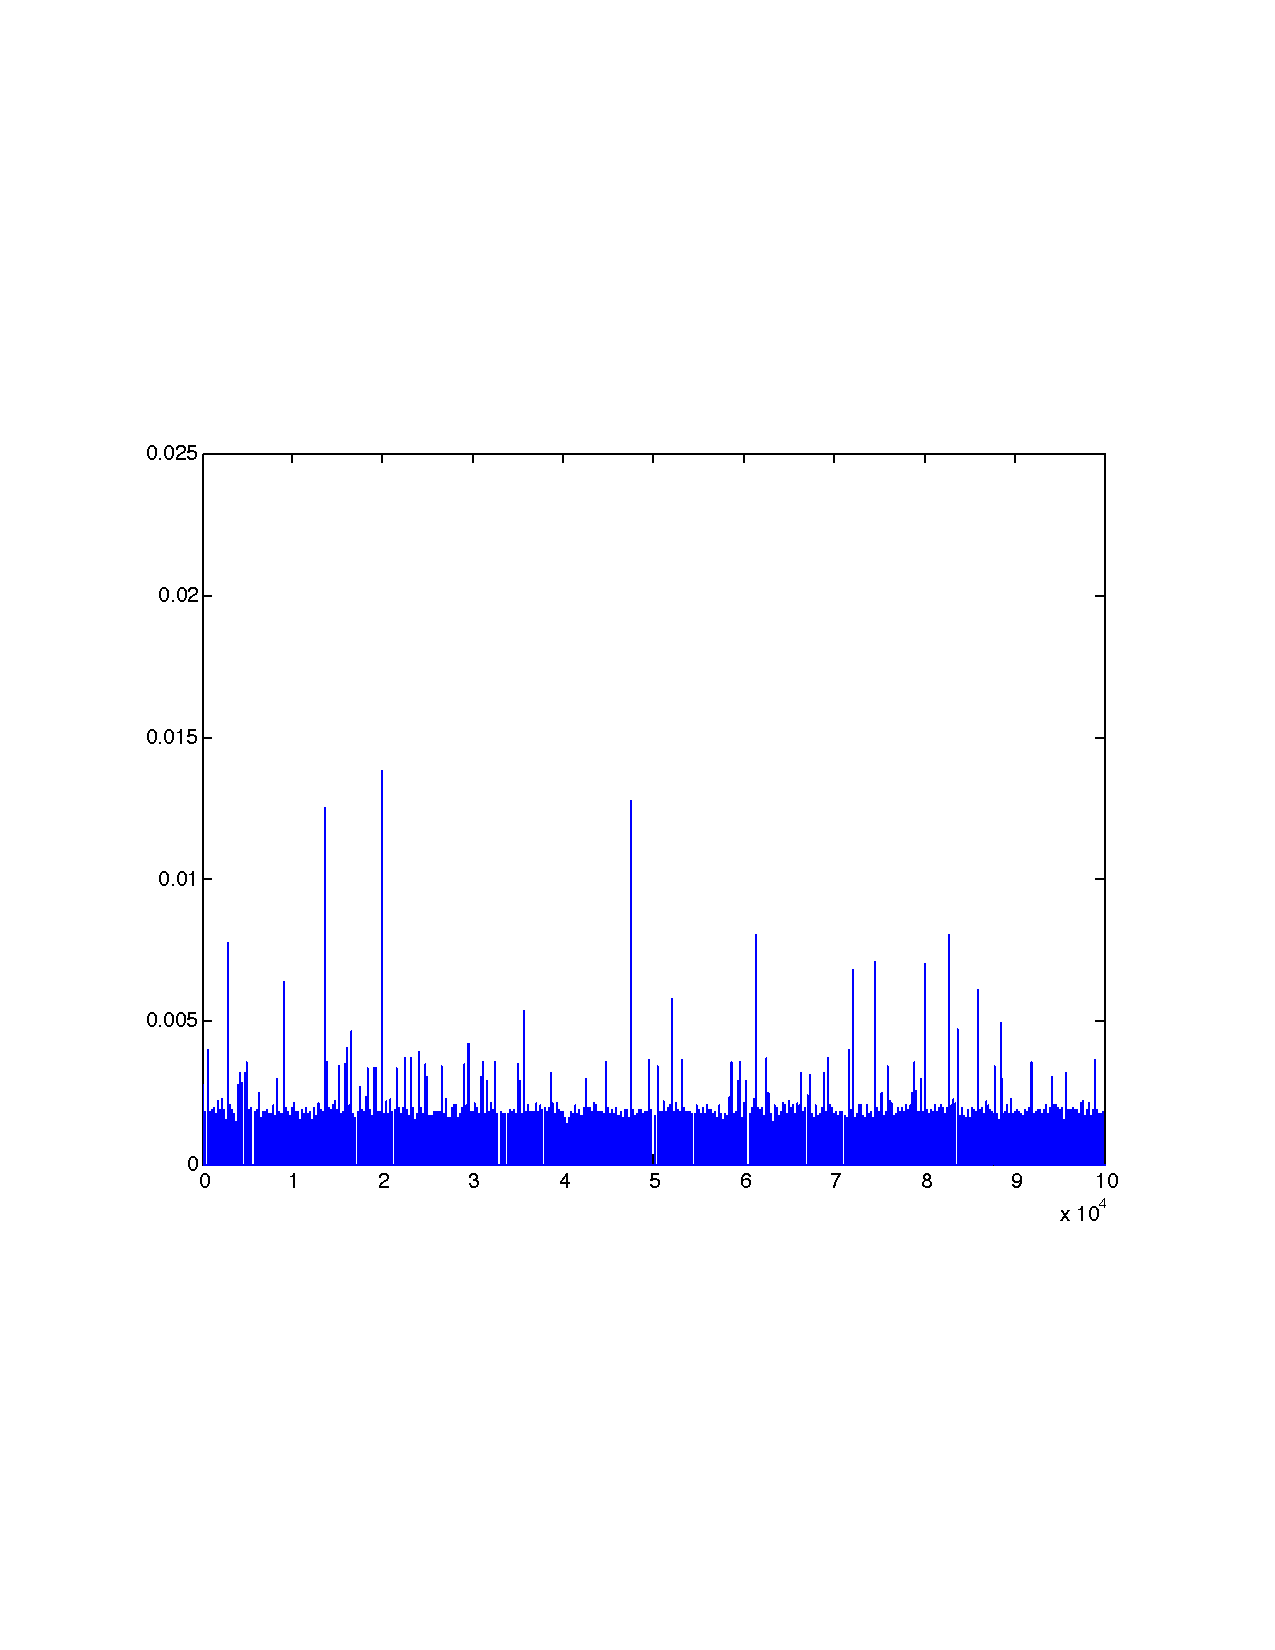
\includegraphics[width=0.3\textwidth]{images/tb_city_hall_weighted.pdf}}
\\
\subfloat[Tower Bridge image 2]{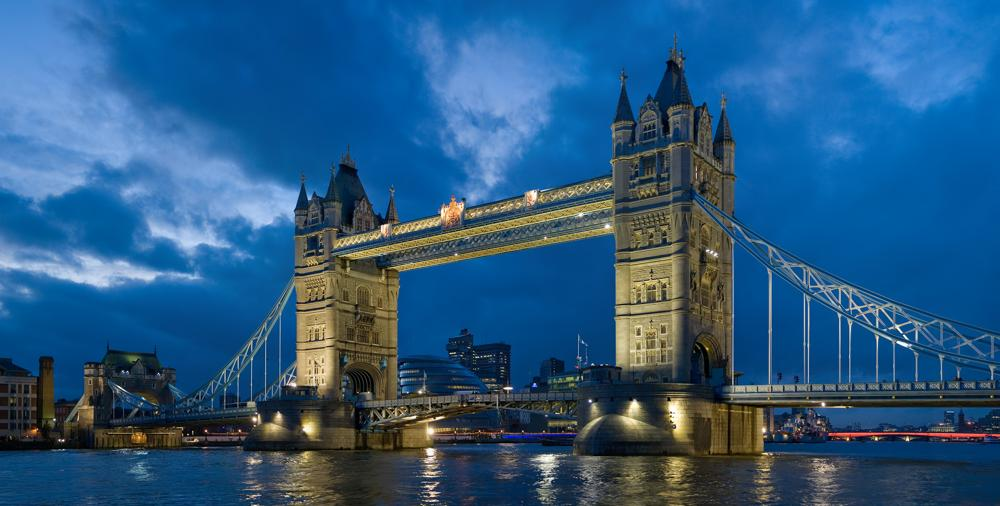
\includegraphics[width=0.3\textwidth]{images/tb_twilight.jpg}}
~
\subfloat[Raw histogram for image 2]{\label{fig:rawhist2}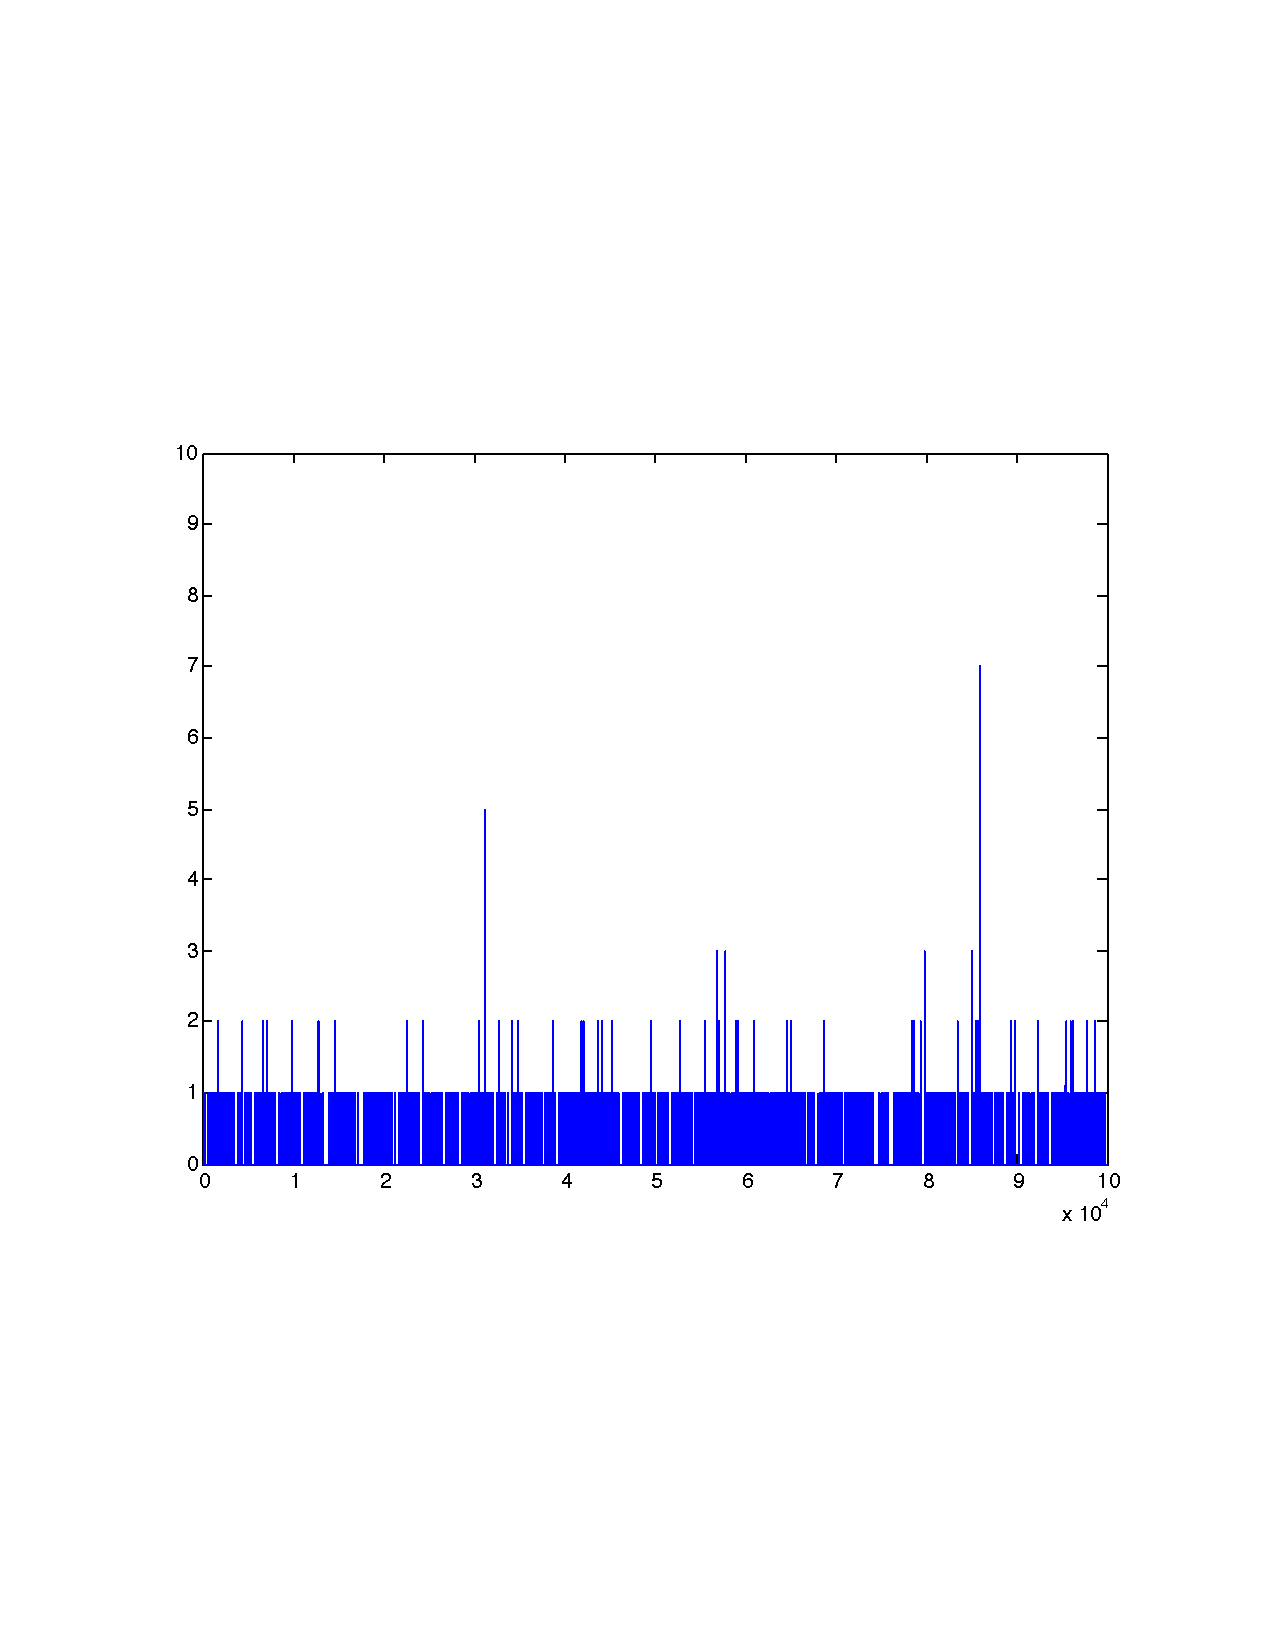
\includegraphics[width=0.3\textwidth]{images/tb_twilight.pdf}}
~
\subfloat[Weighted histogram for image 2]{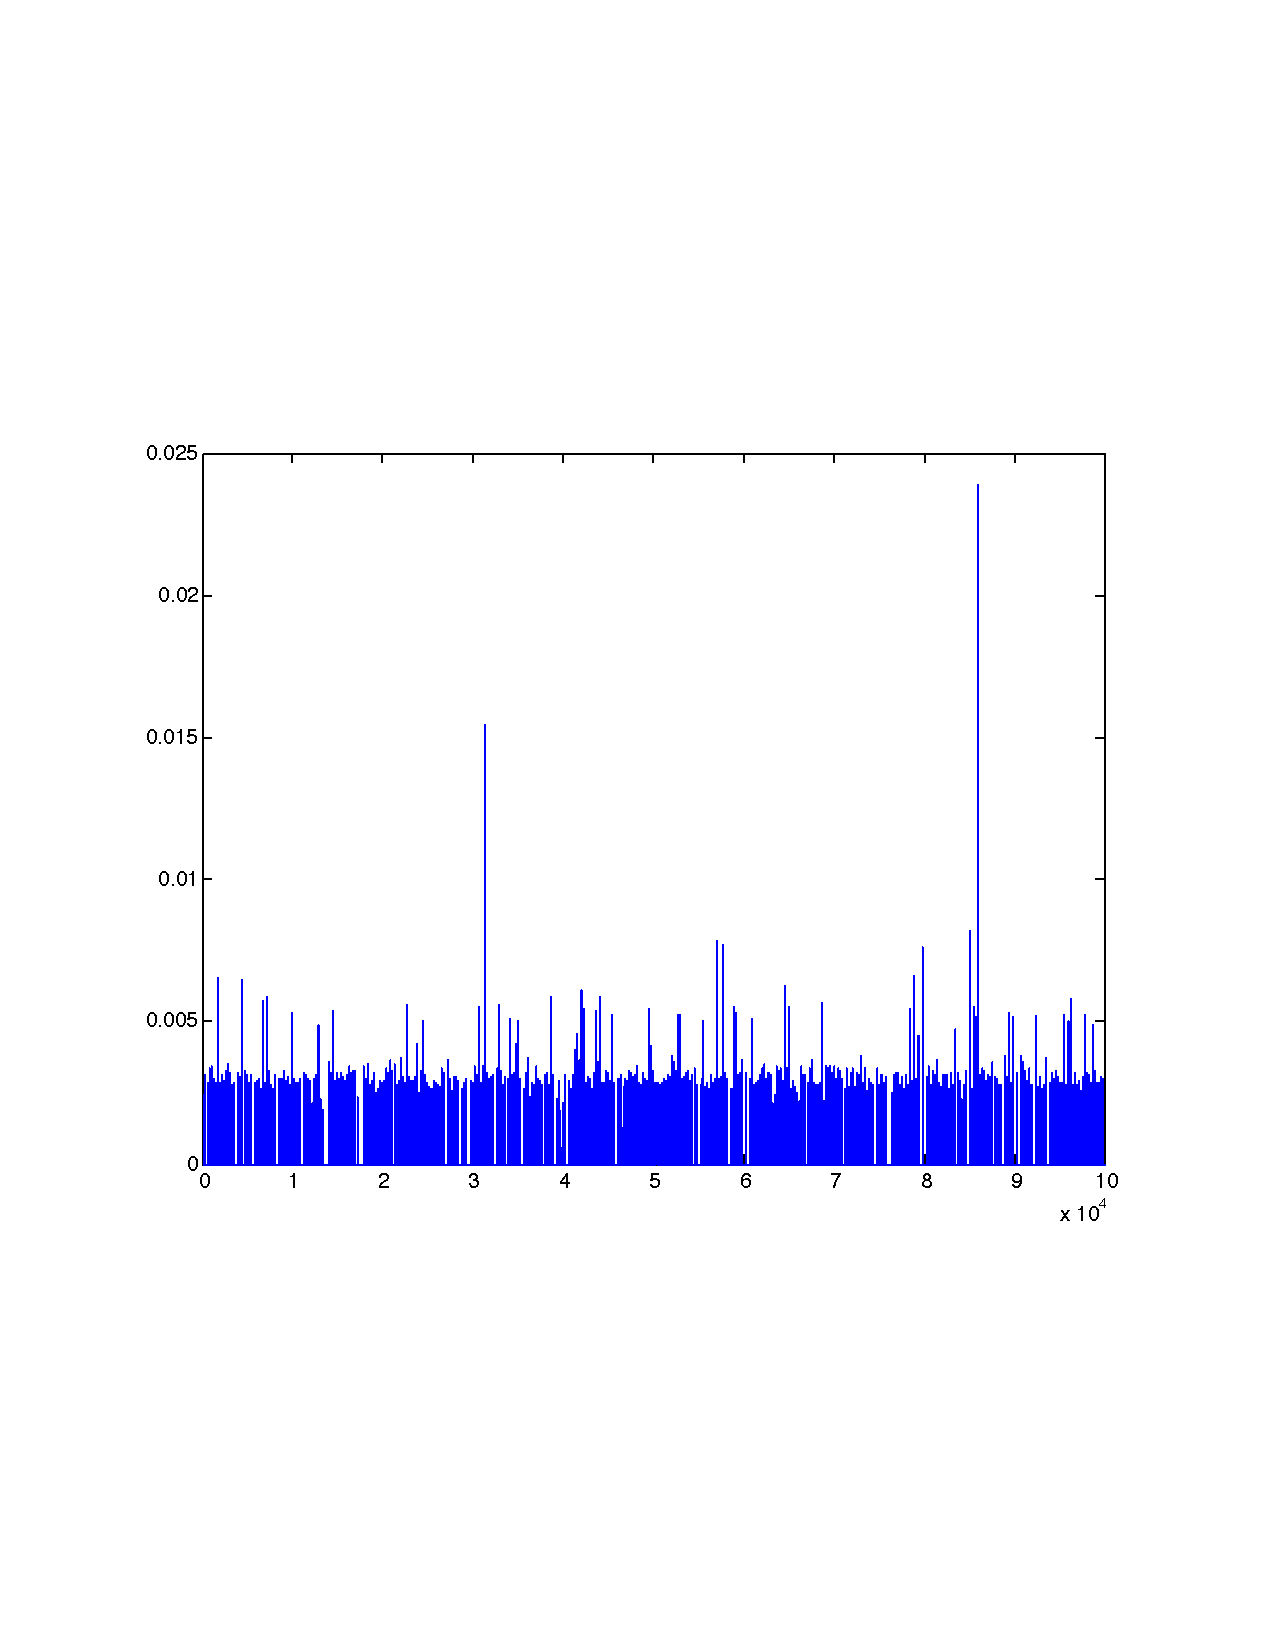
\includegraphics[width=0.3\textwidth]{images/tb_twilight_weighted.pdf}}
\caption{Two images for the class \lstinline!Tower_Bridge! with their raw histograms and tf-idf weighted histograms}
\label{fig:histograms}
\end{figure}

Each model image therefore has a histogram that is used for matching. All the histograms are packaged into a matrix (each column being an image's histogram) that is used as the index for query matching.

To find the most similar images to a query image, a dot product is performed between each of the model image histograms and the query image histogram,
\begin{equation}
\mathbf{scores}= \mathbf{h_{query}^T}
\left[ \begin{array}{ccccc}
\mathbf{h_1} & \mathbf{h_2} & \cdots & \mathbf{h_{N-1}} & \mathbf{h_N}
\end{array}\right]
\label{eqn:tfidfscore}
\end{equation} 
where $\mathbf{h_{query}}$ is the tf-idf weighted histogram of the query image and $\mathbf{h_i}$ is the tf-idf weighted histogram of model image $i$. $\mathbf{scores}$ is a $N\times1$ array with the result of the dot product with each model image's histogram in each element. The matches are ranked in decreasing order of their score -- the model image with the highest score is said to be the most similar to the query image.


\section{Spatial Verification}
\label{sec:spatialverification}
Matching based purely on the tf-idf weighted histograms is effective, however it is prone to false positives. This is due to the fact that two different objects may have very similar features (and therefore many similar visual words), but these features are in very different places as they are not the same object. Therefore, a final spatial verification must be done to ensure that the visual words that appear both in the query image and the model image form the same rigid bodied object.

The spatial verification restraint in this application is that there should exist an affine transformation between the scene in the query image and the scene in the model image that is the potential match. Practically, this means that there should be an affine transformation that maps the visual words in the query image to the position of the same visual words in the model image. Equation~\ref{eqn:affine} shows this transformation, such that $\mathbf{x'}$ is the positions of the visual word in the model image, $\mathbf{x}$ is the position of the visual word in the query image, and $\mathbf{H}$ is the affine transformation between the two images.

\begin{equation}
\mathbf{x'}=
\left[ \begin{array}{c}
x' \\
y' \\
1
\end{array}\right]
=
\left[ \begin{array}{ccc}
a & b & t_x \\
c & d & t_y \\
0 & 0 & 1
\end{array}\right]
\left[ \begin{array}{c}
x \\
y \\
1
\end{array}\right]
= \mathbf{H}\mathbf{x}
\label{eqn:affine}
\end{equation} 

The random sample consensus algorithm (RANSAC) is used to estimate an affine transformation between the two images, using the corresponding visual words in each image. All duplicate visual words are removed from the spatial verification process, as these duplicates often cause inaccurate estimations. The result of the RANSAC spatial verification is the number of visual words in the query image that map to the correct positions in the model image (within some tolerance region). Matches that have enough inliers under the transformation are said to be spatially verified -- that is the estimated affine transformation is accurate and both images depict the same rigid bodied object.

\begin{figure}[h!tb]
\centering 
\subfloat[Big Ben image 1]{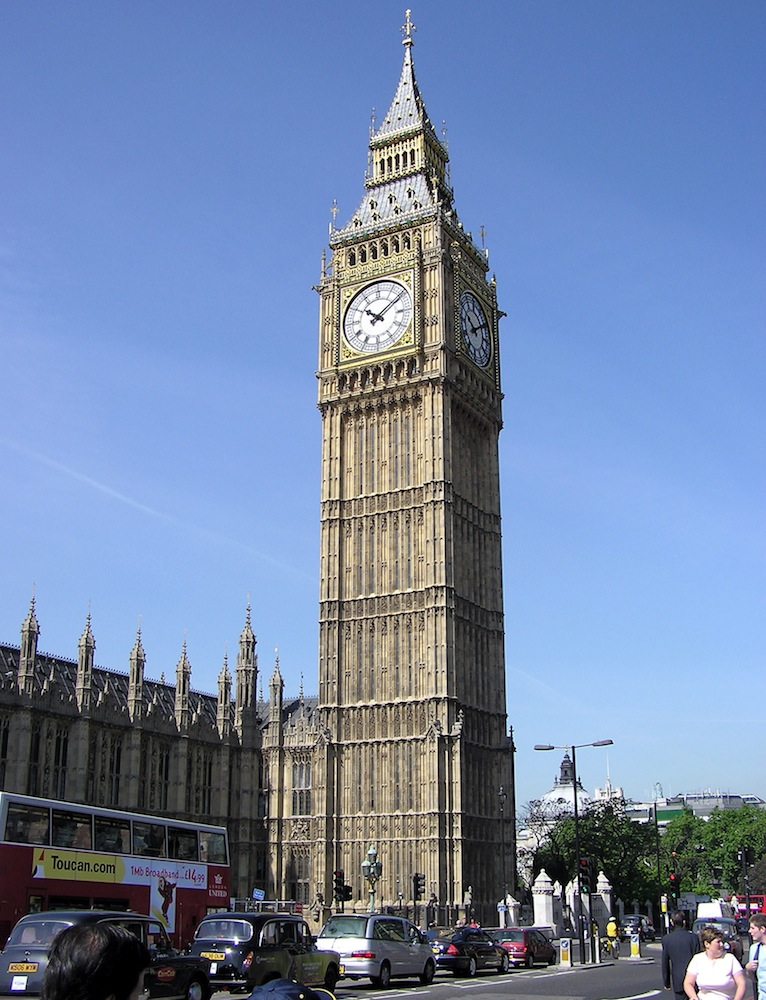
\includegraphics[width=0.18\textwidth]{images/bigben.jpg}}
~
\subfloat[Big Ben image 2]{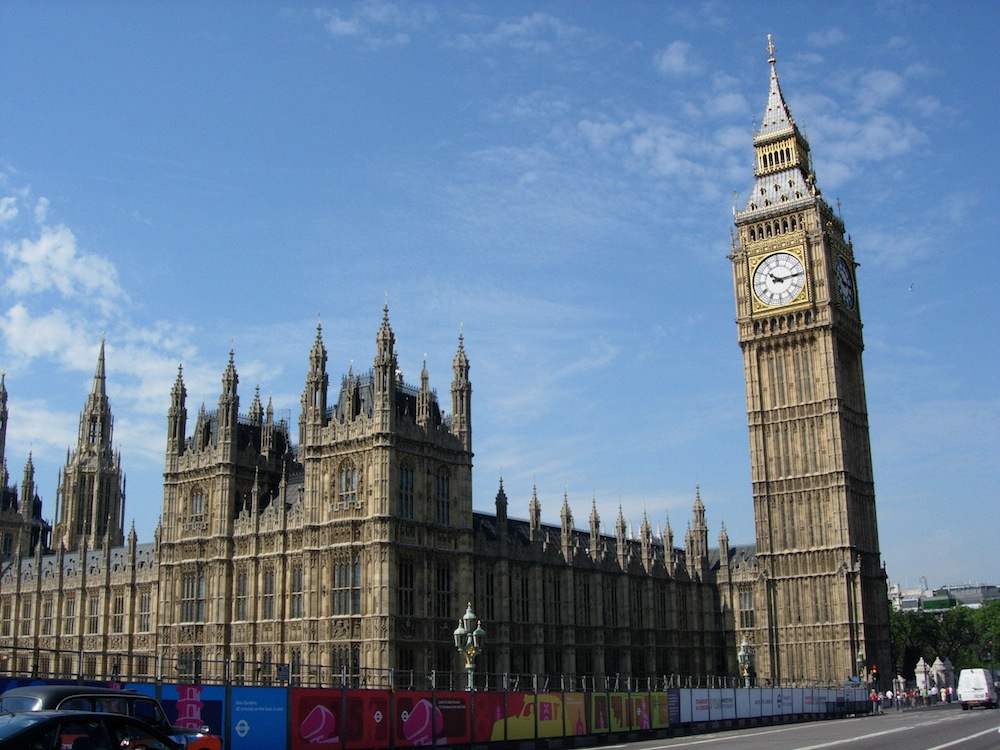
\includegraphics[width=0.3\textwidth]{images/bigben2.jpeg}}
\\
\subfloat[Matches based purely on SIFT feature similarity]{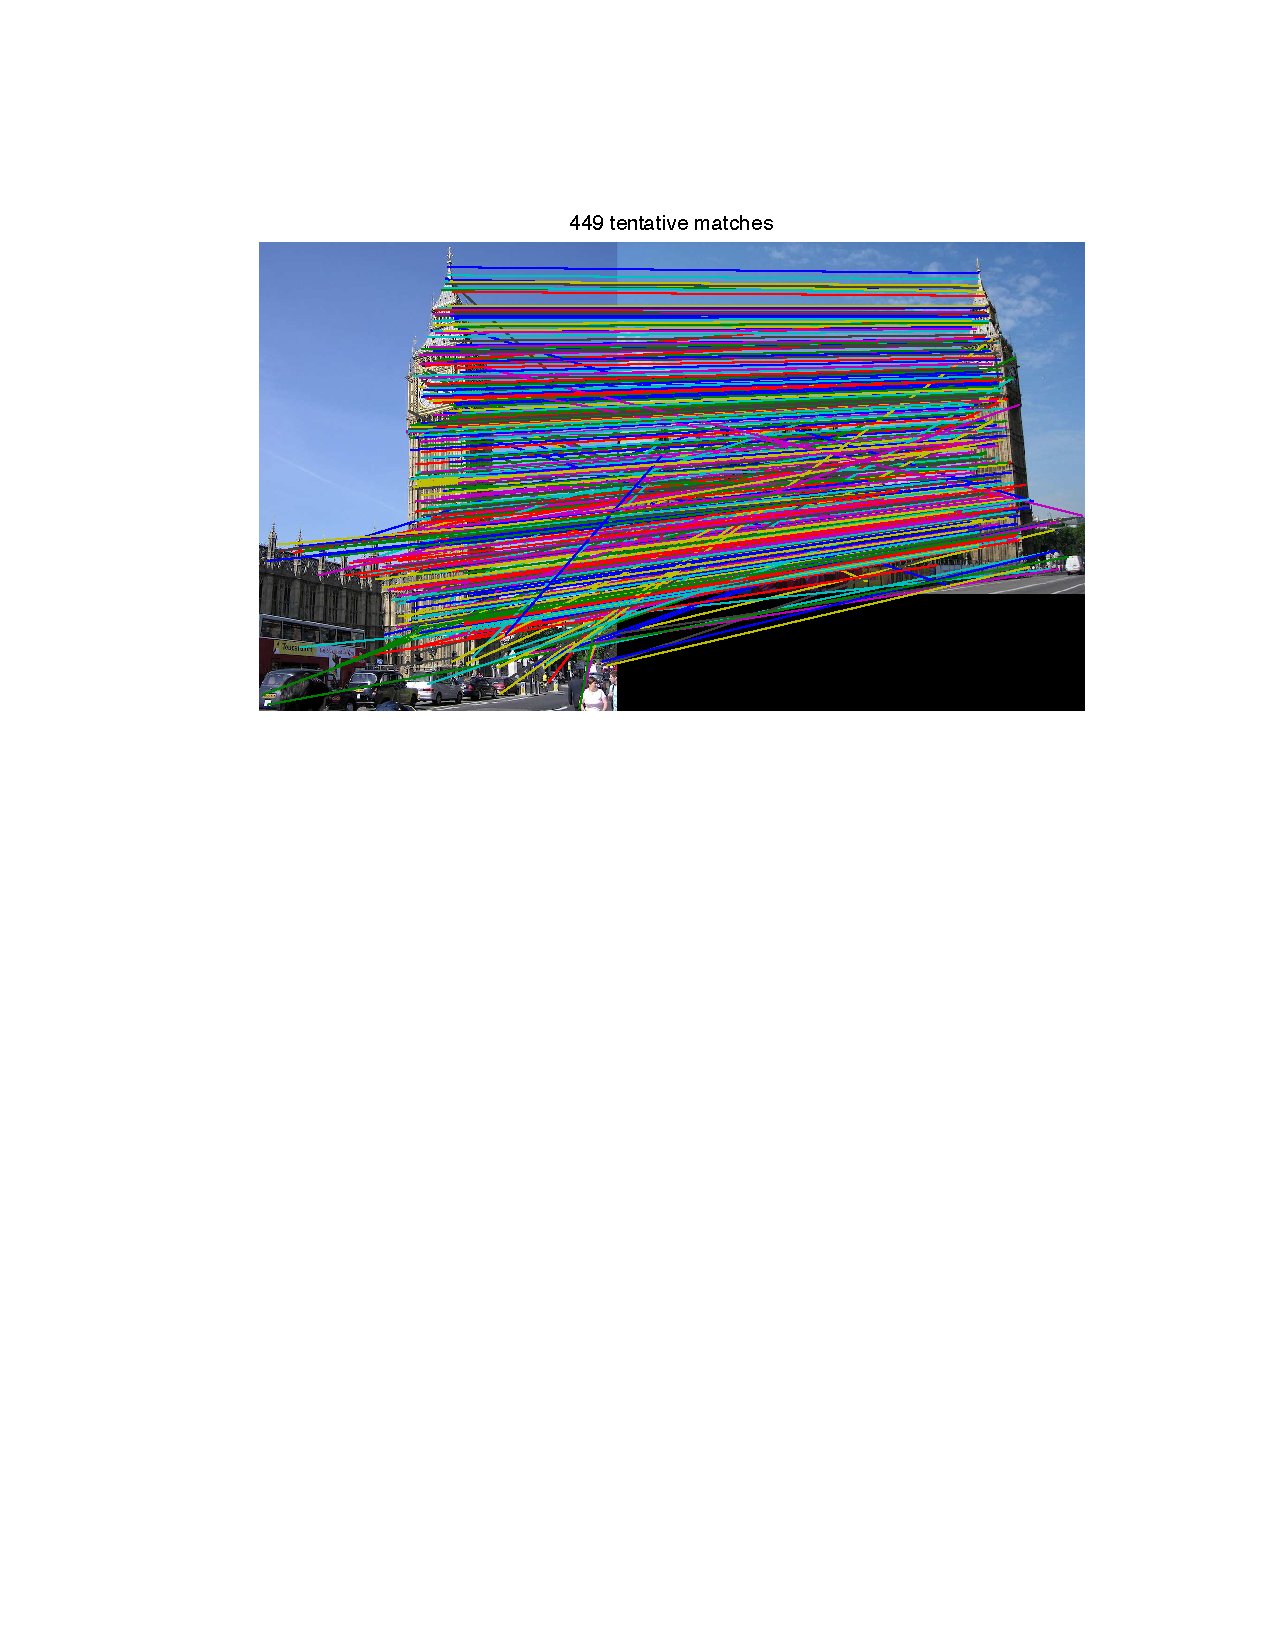
\includegraphics[width=0.4\textwidth]{images/spatial_verification1.pdf}}
\subfloat[Matches after RANSAC spatial verification]{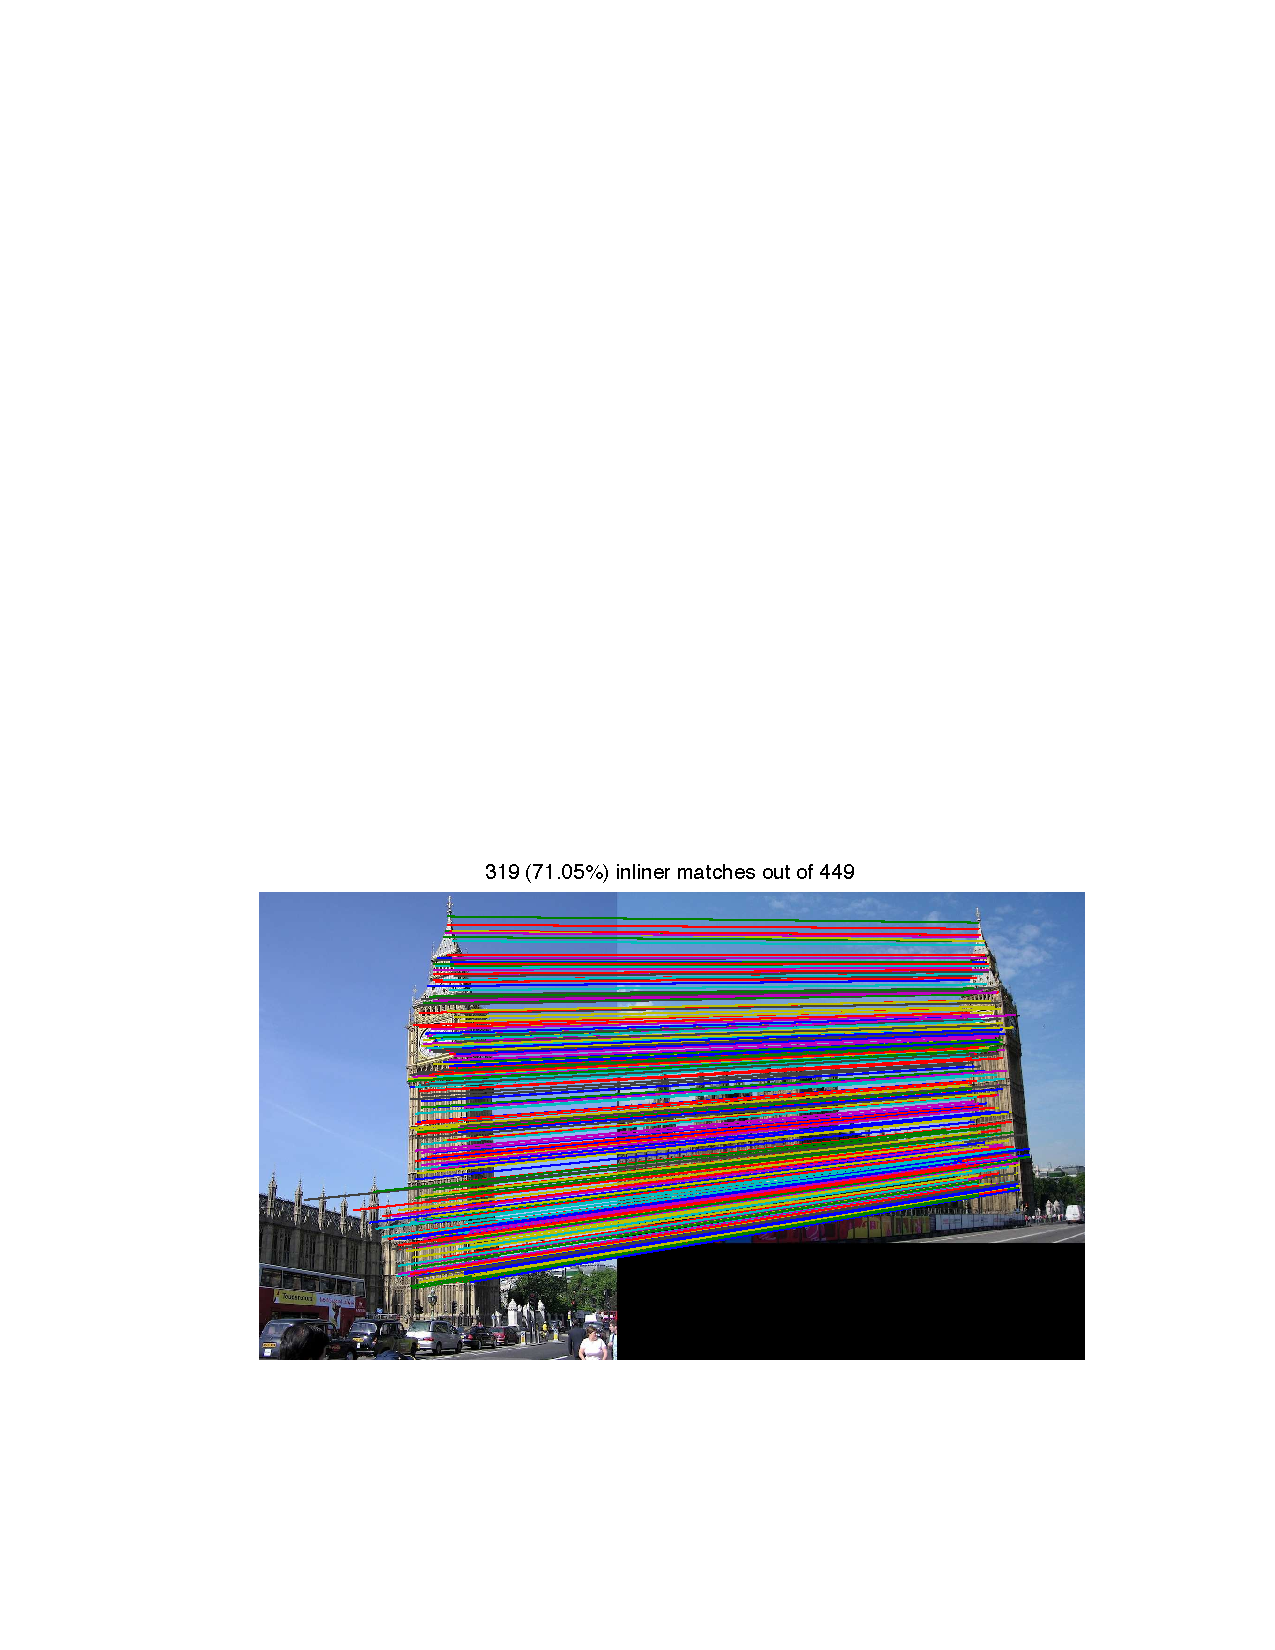
\includegraphics[width=0.4\textwidth]{images/spatial_verification2.pdf}}
\caption{RANSAC spatial verification performed on two images of Big Ben.}
\label{fig:spatialverification}
\end{figure}

Figure~\ref{fig:spatialverification} shows the result of spatial verification on matched SIFT features. Note the disregarding of some matches after RANSAC as these matches do not conform with the estimated affine transformation.

Spatial verification is performed on each model image in descending order of the tf-idf histogram matching score. The first model image to be successfully spatially verified is deemed to be an accurate match and the process is terminated, with the class the model image represents being the object found. The region of the query image that is labelled as the object is the bounding box of visual words that spatially match the model image.


\section{Multiple Object Matching}
\label{sec:multiobject}
The object recognition engine can recognise multiple objects in a single image (an example is shown in Figure~\ref{fig:multiplematching}). Once an object has been successfully recognised, the query is re-issued with the same query image, however the visual words contained within the regions of already recognised objects are excluded from the query process. Previously recognised objects are ignored as matches from the re-issued queries and the process finishes when no new objects can be found. 

This method allows any number of objects to be recognised within a single image. The downside of this process is that it requires multiple queries so increases the time taken to complete.

\begin{figure}[htb]
\centering 
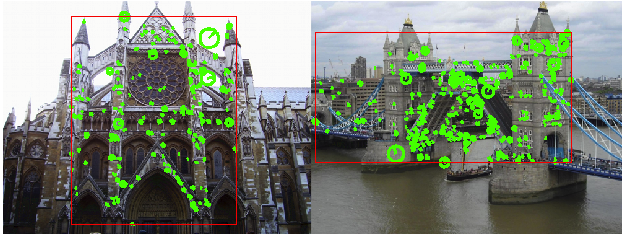
\includegraphics[width=0.7\textwidth]{images/multimatch.png}
\caption{An artificially created image showcasing multiple object matching.}
\label{fig:multiplematching}
\end{figure}

\section{Performance}
The baseline system was tested to obtain a measure of the object recognition performance. The best achievable yield (see Section~\ref{sub:performance}) was 18.1\%. This is fairly low for this sort of application. There are a number of limitations in the matching process, such as with the spatial verification, as well as the lack of representative images that are the root cause of this performance.

%-------------------------------
% Geometric Improvements
%-------------------------------
\linespread{1}\chapter{Geometric and Descriptor Improvements}
\label{chpt:geoimprovements}

A number of modifications to the baseline system were explored to increase the matching performance of the object recognition system. These improvements are using the NOSAC algorithm in place of RANSAC (Section~\ref{sec:nosac}), using a different feature detector and transformation estimation algorithm based on affine invariant feature regions (Section~\ref{sec:affine}), and modifying the descriptors to improve conditioning (Section~\ref{sec:rootsift}).

\section{NOSAC}
\label{sec:nosac}
To estimate an affine transformation between two images, six variables must be estimated ($a$, $b$, $c$, $d$, $t_x$, and $t_y$ in Equation~\ref{eqn:affine}). 
Each feature point that is computed for an image contains four data points: the $x$ coordinate, $y$ coordinate, scale $s$, and rotation $\theta$ of the feature. The baseline RANSAC method randomly selects three correspondences and uses the $x$ and $y$ coordinates to yield two equations for each correspondence. For three correspondences, that means there are six equations, so the transformation can be solved. The best transformation (the one with the most inliers) over all the iterations of sampling is then used as a basis for the overall affine transformation.

\begin{figure}[htb]
\centering 
\subfloat[RANSAC]{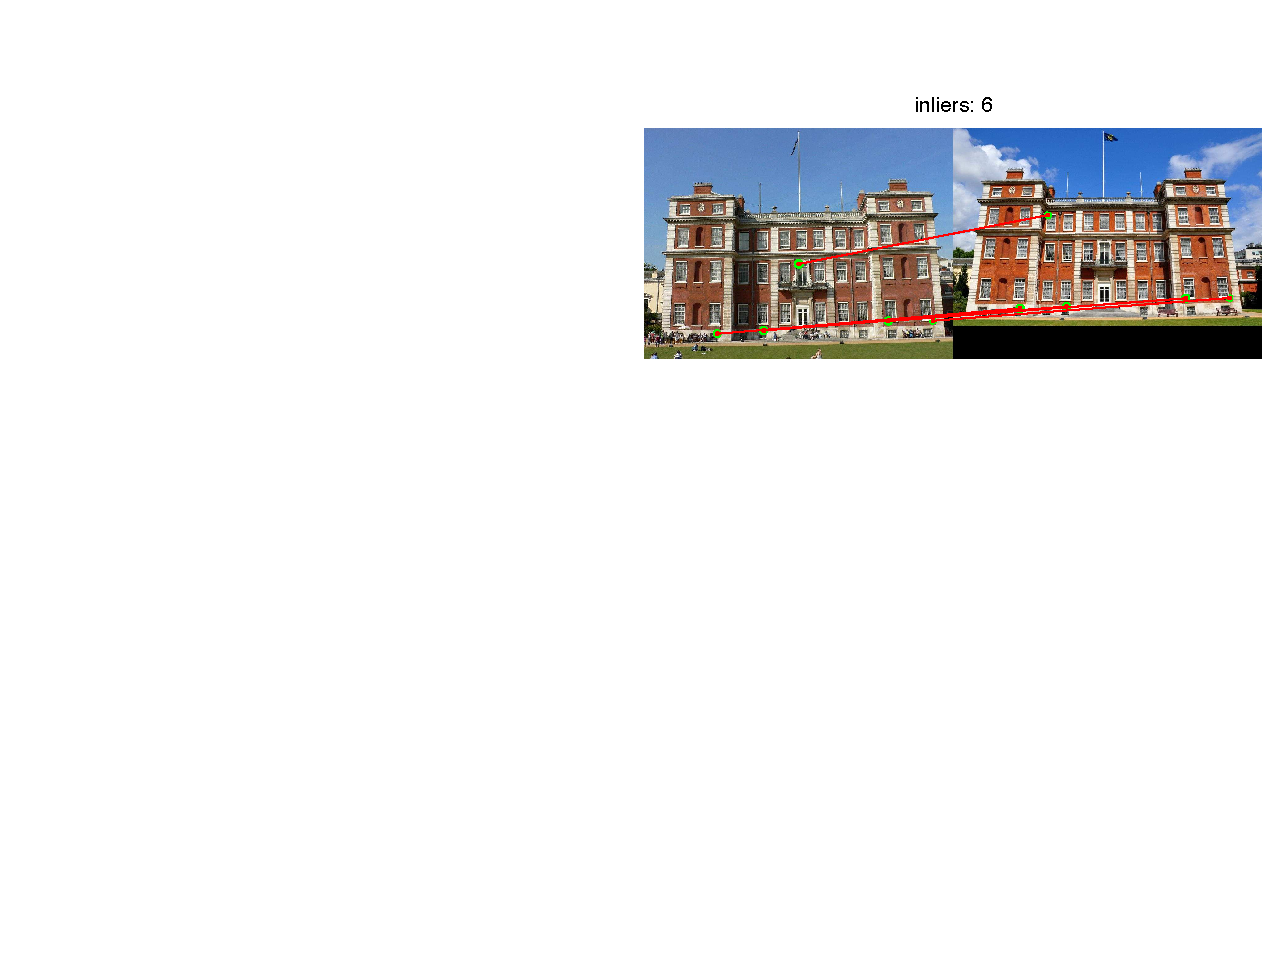
\includegraphics[width=0.7\textwidth]{images/ransacmatch.pdf}}
\\
\subfloat[NOSAC]{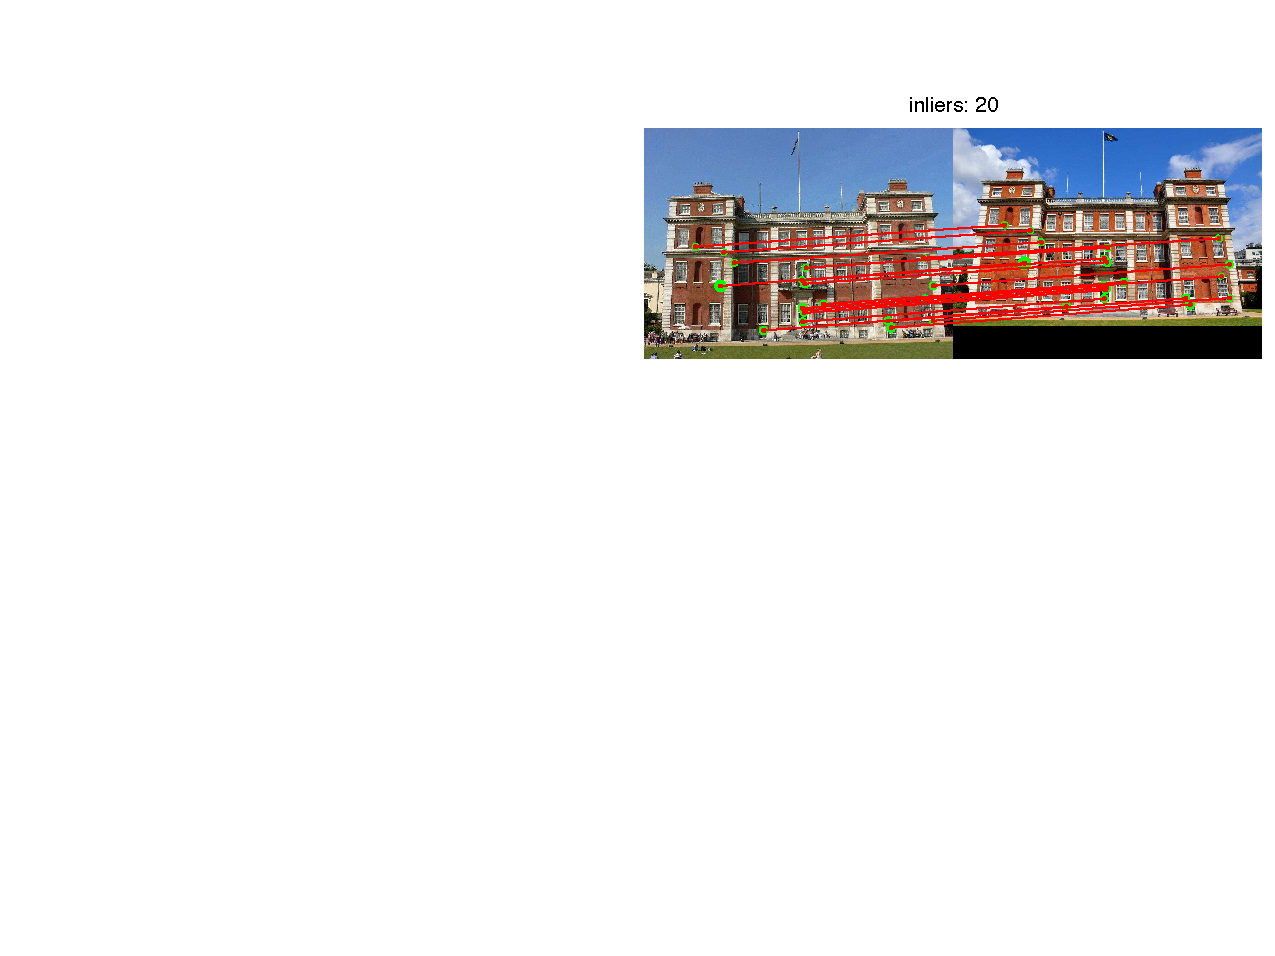
\includegraphics[width=0.7\textwidth]{images/nosacmatch.pdf}}
\caption{The difference in matching by using NOSAC compared to RANSAC}
\label{fig:ransacnosac}
\end{figure}

This method works well, however it is based on random sampling so either accuracy or speed is sacrificed. Instead, a new estimation method is used called NOSAC. 

Rather than selecting three correspondences, only one correspondence is needed to estimate a transformation. Initially, it is assumed the only components of the transformation are scaling and translation, as shown in Equation~\ref{eqn:scaleaffine}. There are therefore only three unknown variables -- $a$, $t_x$, and $t_y$. The scaling factor $a$ is estimated from the relative scales of the feature points, and the translation from the coordinates. An estimation is done for every correspondence. The inliers of the best estimation of the transformation are then used to compute the full six degree of freedom affine transformation\footnote{This is done using \lstinline$vgg_Haffine_from_x_MLE$ by Andrew Zisserman found on \url{http://www.robots.ox.ac.uk/~vgg}}. 

\begin{equation}
\mathbf{x'}=
\left[ \begin{array}{ccc}
a & 0 & t_x \\
0 & a & t_y \\
0 & 0 & 1
\end{array}\right]\mathbf{x}
\label{eqn:scaleaffine}
\end{equation} 

\linespread{1} % single line spacing
\lstset{language=Matlab,caption=Estimating the pure scale affine transformation for each corresponding feature.,label=lst:nosac}
\begin{lstlisting}[frame=single]
%% MATLAB
% for each correspondence
for i=1:n_correspondences
    % compute transformation (a 0 tx; 0 a ty; 0 0 1) where a = s2/s1
    a = f2(3,i)/f1(3,i);
    T = f2(1:2,i) - s*f1(1:2,i);
    H{i} = [s 0 T(1); 0 s T(2); 0 0 1]; 
    % score all the other points from transformation
    X2_ = H{i} * X1;
    delta = X2_ - X2;
    ok_rough{i} = sum(delta.*delta,1) < (1*thresh)^2;
    score_rough(i) = sum(ok_rough{i});
end\end{lstlisting}
\linespread{2} % double line spacing

As an estimation is performed on every correspondence, there is no randomness to the process. Also, as the number of iterations is the number of correspondences, the NOSAC method is considerably faster than RANSAC. Matching performance is increased by 15\% compared to that of the baseline system, to an absolute yield of 20.8\%.

\section{Affine Invariant Detector}
\label{sec:affine}
An alternative feature detector is used as an improvement. The Hessian affine region detector detects regions similar to the SIFT detector of the baseline system. However, the features detected are affine invariant -- the detector will detect the same features and describe them in the same way even if the viewpoint has changed. This has the advantage of allowing matching of features even when the viewpoint of the object is markedly different.

\begin{figure}[h!tb]
\centering 
\subfloat[NOSAC]{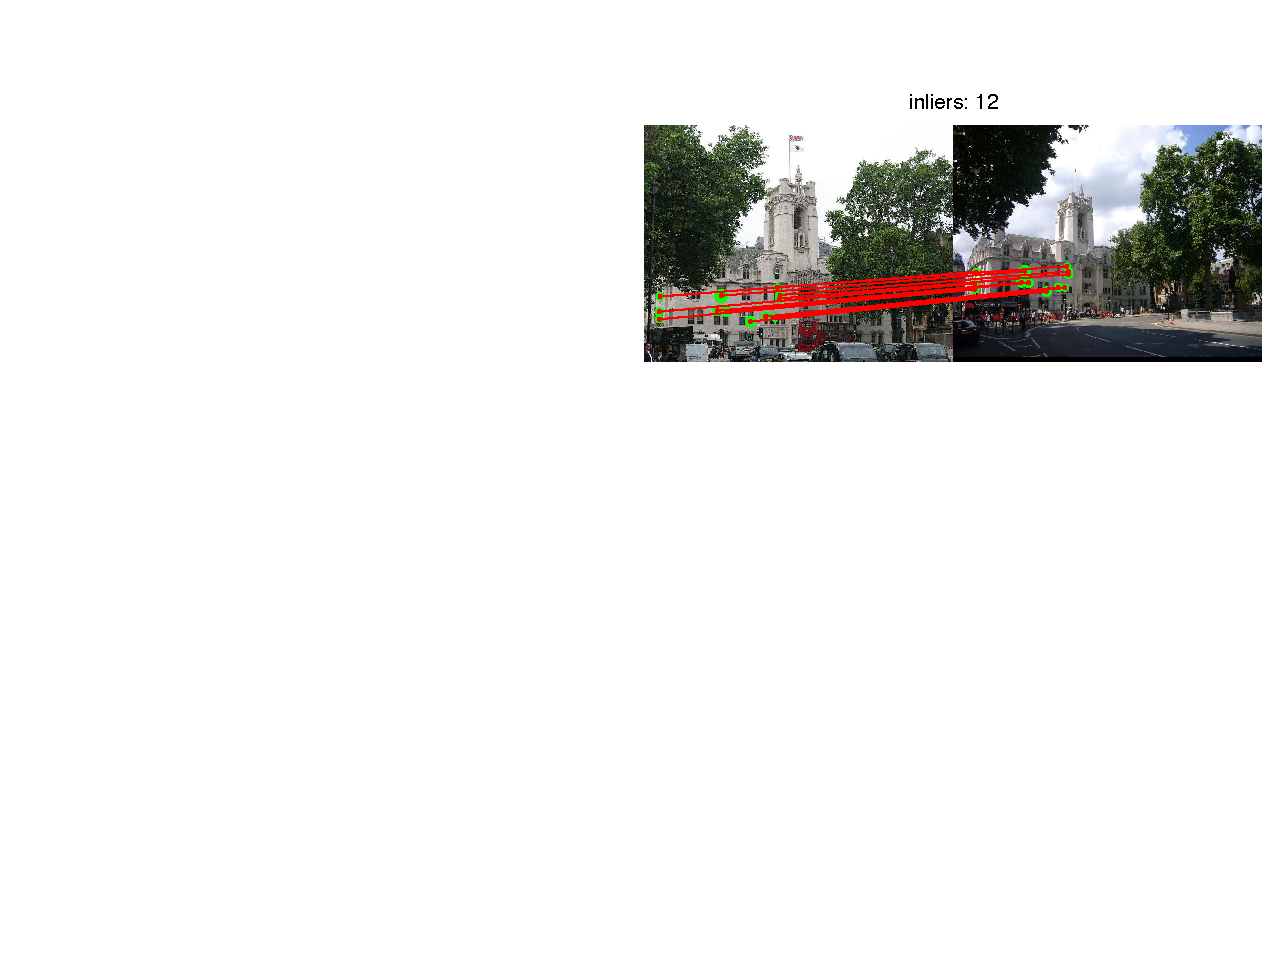
\includegraphics[width=0.65\textwidth]{images/nosacmatch2.pdf}}
\\
\subfloat[Affine Invariant]{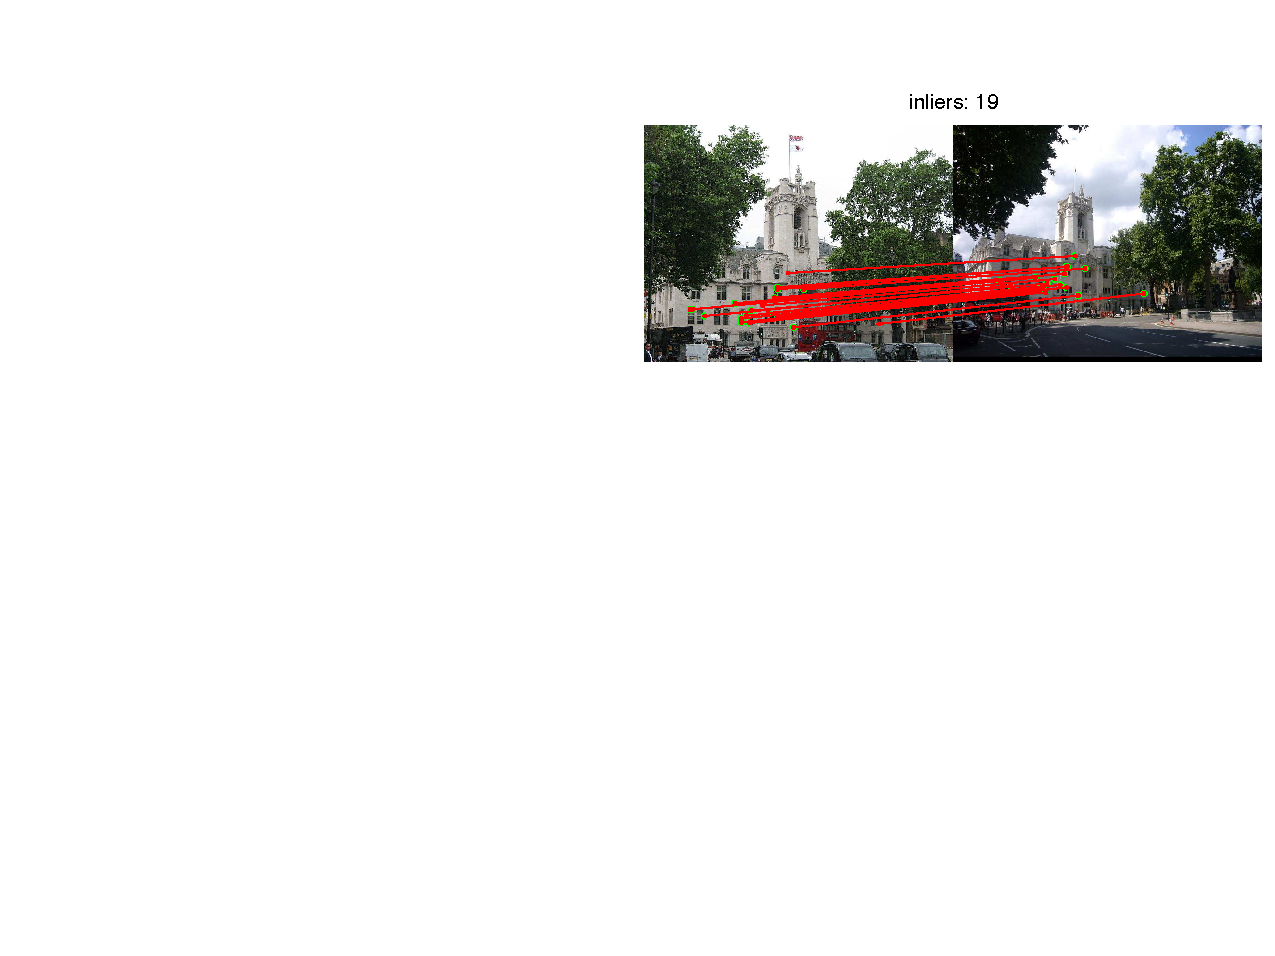
\includegraphics[width=0.65\textwidth]{images/affinematch.pdf}}
\caption{The difference in matching by using the affine invariant feature detector compared to NOSAC.}
\label{fig:affinenosac}
\end{figure}

The feature points are now six-dimensional rather than four-dimensional, with each feature region being described by its $x$ and $y$ position, orientation $\theta$ and the ellipse representing the region, given by three parameters $a$, $b$ and $c$ such that the ellipse is described by 
\begin{equation}
ax^2 + 2bxy + cy^2 = 
\left[ \begin{array}{cc}
x & y
\end{array}\right]
\left[ \begin{array}{cc}
a & b \\
b & c
\end{array}\right]
\left[ \begin{array}{c}
x\\
y
\end{array}\right]
=
\mathbf{x^T}\mathbf{S}\mathbf{x}
= 0.
\label{eqn:ellipse}
\end{equation} 

There are two advantages of using the affine invariant detector. The first is that there are more corresponding visual words between images of the same object as the features from a different viewpoints are always detected, and described in the same way. 

The second is that better estimations of the affine transformation can be done during the NOSAC process. However, rather than assuming purely scaling and translation as in Section~\ref{sec:nosac}, a full affine transformation can be computed for each correspondence. This is because each feature is described by an ellipse. For a correspondence between two points with ellipses described by
\begin{equation}
\mathbf{x_1^T}\mathbf{S_1}\mathbf{x_1}= 0
\label{eqn:ellipse1}
\end{equation} 
and
\begin{equation}
\mathbf{x_2^T}\mathbf{S_2}\mathbf{x_2}= 0
\label{eqn:ellipse2}
\end{equation} 
related by
\begin{equation}
\mathbf{x_2} = \mathbf{H}\mathbf{x_1}
\label{eqn:elaffine}
\end{equation} 
the unknown affine transformation $\mathbf{H}$ can be found by solving
\begin{equation}
\mathbf{S_1} = \mathbf{H^T}\mathbf{S_2}\mathbf{H}
\label{eqn:elaffine}
\end{equation} 
given the constraint that vertical is mapped to vertical (see Section~4.1 in \cite{philbin2007}).

As with NOSAC, this is done for every correspondence and the inliers from the best estimation used to compute a final estimate for the transformation. The process is faster than RANSAC and also results in a 24\% increase in yield compared to the baseline system's yield, giving an absolute yield of 22.5\%.


\section{RootSIFT}
\label{sec:rootsift}

\begin{figure}[h!]
\centering 
\subfloat[Affine Invariant SIFT]{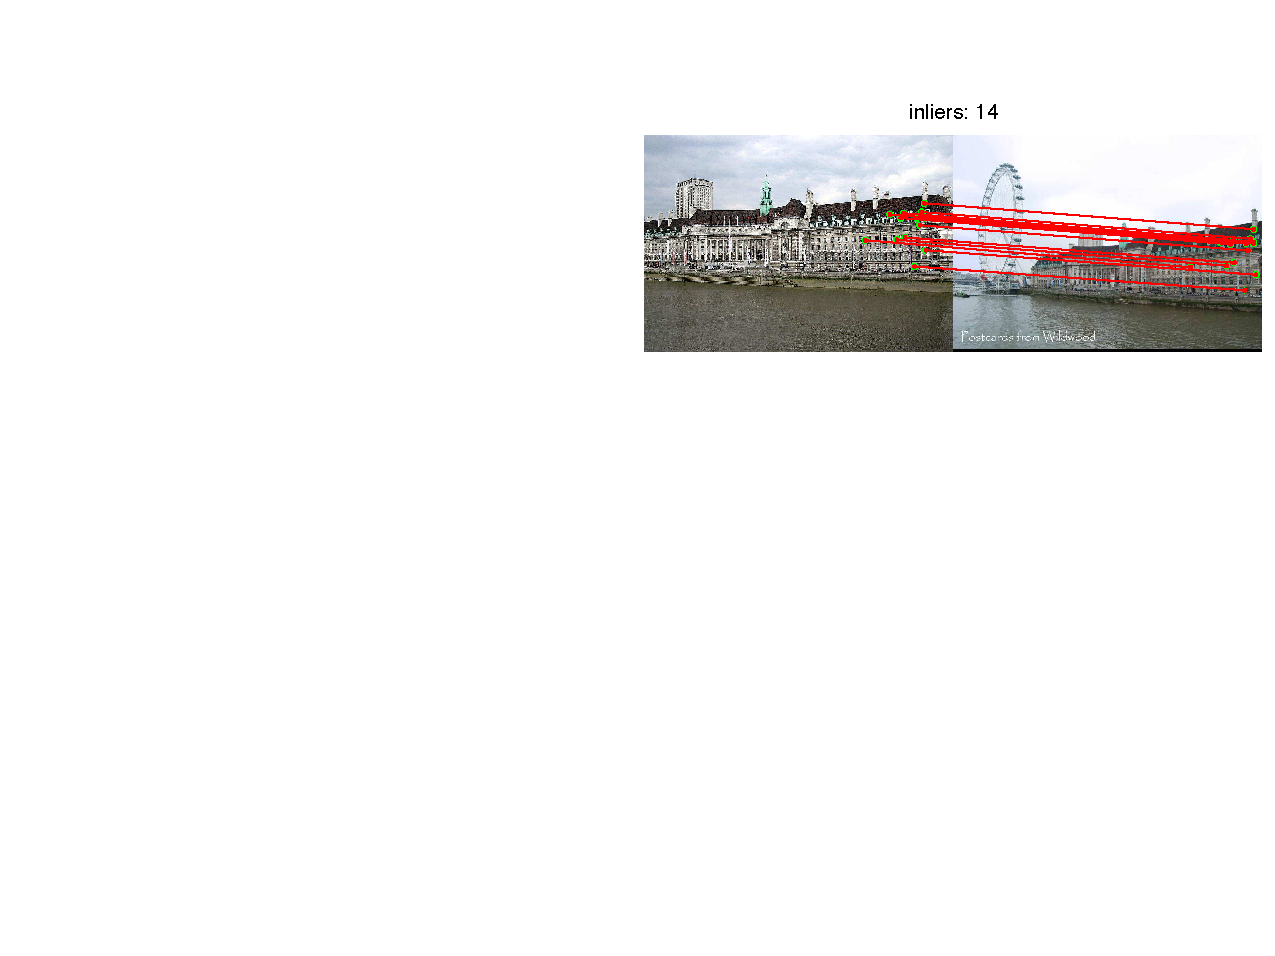
\includegraphics[width=0.7\textwidth]{images/affinematch2.pdf}}
\\
\subfloat[Affine Invariant RootSIFT]{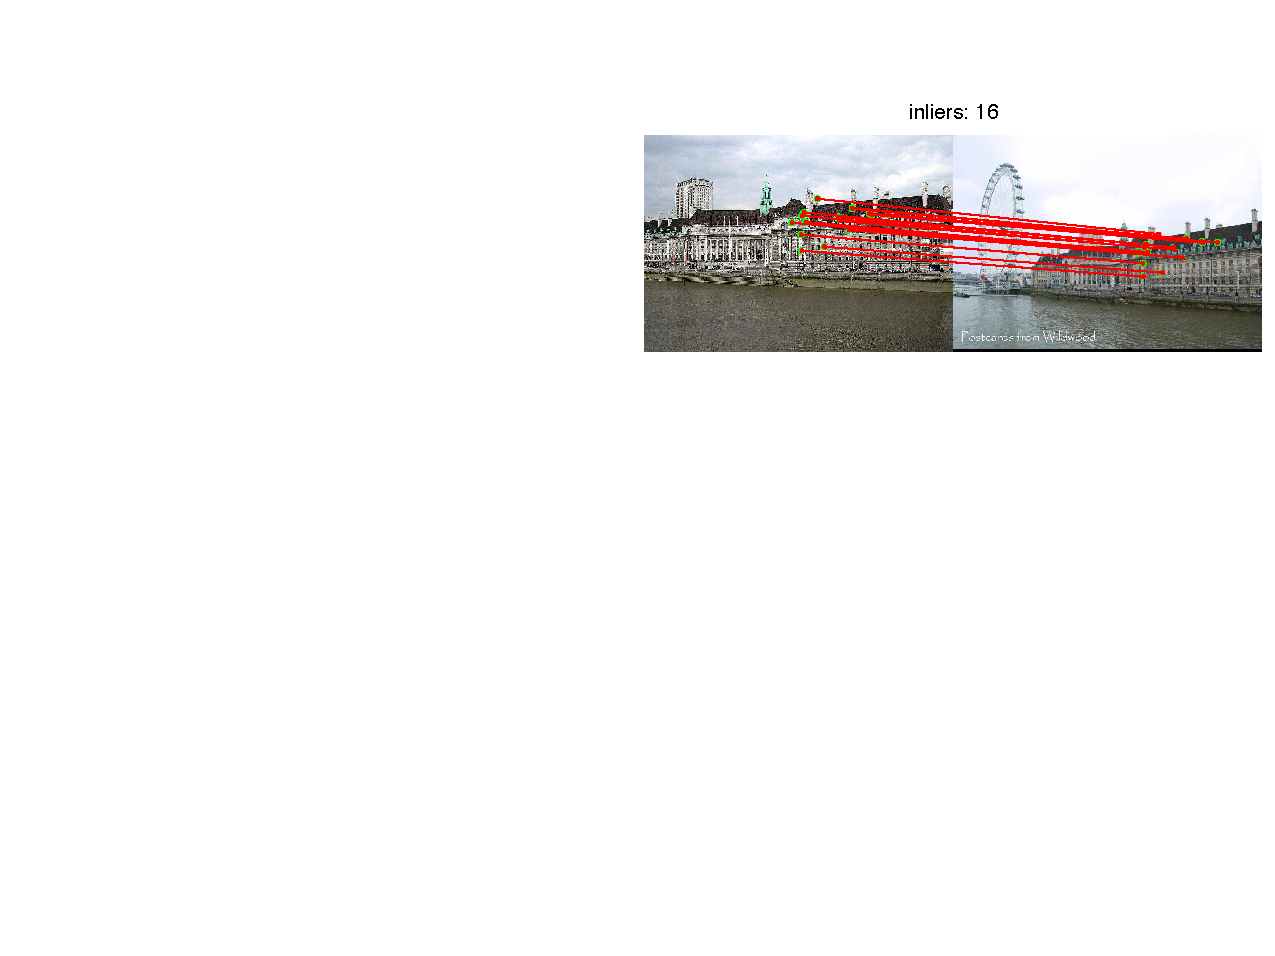
\includegraphics[width=0.7\textwidth]{images/rootaffinematch.pdf}}
\caption{The difference in matching by using RootSIFT descriptors as compared vanilla SIFT.}
\label{fig:affinerootaffine}
\end{figure}

To measure the similarity between two features, the Euclidean distance between the SIFT descriptors is used in the baseline system. However, a recent publication \cite{rootsift12} notes that using a different distance measure can increase performance.

The Hellinger kernel is used in place of the standard Euclidean kernel for computing distance. This change can be performed by simply mapping the descriptors from SIFT space to RootSIFT space -- the RootSIFT descriptor is an element wise square root of the L1 normalised SIFT vector. Computing the Euclidean distance between two RootSIFT vectors is equivalent to using the Hellinger kernel for comparing the original SIFT descriptors. Listing~\ref{lst:rootsift} shows the conversion of the SIFT descriptor \lstinline!sift! to RootSIFT space.

\linespread{1} % single line spacing
\lstset{language=Matlab,caption=Mapping of SIFT descriptors to RootSIFT space.,label=lst:rootsift}
\begin{lstlisting}[frame=single]
%% MATLAB
root_sift = sqrt(sift/sum(sift));
\end{lstlisting}
\linespread{2} % double line spacing


The effect of using RootSIFT is to reduce the larger SIFT dimensions in relation to the smaller ones. This prevents the Euclidean distance being dominated by these large values, which could be noisy. By using RootSIFT space with the affine invariant detector, matching performance is increased 35\% compared to the baseline system, giving an absolute yield of 24.5\%



\section{Results}
The results of these geometric improvements is shown in Table~\ref{tbl:improvements}. 

Recalled from Chapter~\ref{chpt:system}, the baseline system uses RANSAC to estimate an affine transformation between the query image and model images for spatial verification. If the number of corresponding features that conform to this transformation exceeds a threshold, the inlier threshold, the match is said to be spatially verified. Table~\ref{tbl:improvements} shows the impact on yield (see Subsection~\ref{sub:performance}) by implementing these improvements and varying the inlier threshold.

It is easy to see that implementing the affine invariant detector with the RootSIFT mapping results in the best performance. This is due to the increase in matching accuracy, allowing a lower inlier threshold to be used and so more matches to be made.

\begin{table}[hbtp]
\begin{center}
\begin{tabular}{c|c|c|c|c|}
\cline{2-5}
 & \multicolumn{4}{|c|}{Inlier Threshold} \\ 
 \cline{2-5}
 & 4 & 5 & 7 & 9 \\
 \cline{2-5}
 \cline{1-5}
\multicolumn{1}{|c|}{RANSAC} & \texttt{12.0\%} & \texttt{14.1\%} & \textcolor{red}{\texttt{18.1\%}} & \texttt{14.3\%} \\  
\cline{1-5}
\multicolumn{1}{|c|}{NOSAC} & \texttt{20.7\%} & \textcolor{red}{\texttt{20.8\%}} & \texttt{17.7\%} & \texttt{16.1\%} \\  
\cline{1-5}
\multicolumn{1}{|c|}{Affine} & \textcolor{red}{\texttt{22.5\%}} & \texttt{22.3\%} &  \texttt{17.4\%} & \texttt{13.8\%} \\  
\cline{1-5}
\multicolumn{1}{|c|}{Affine RootSIFT} & \textcolor{red}{\texttt{24.5\%}} & \texttt{22.6\%} &  \texttt{18.0\%} & \texttt{15.5\%} \\  
\cline{1-5}
\end{tabular}
\end{center}
\caption{The yield acheived for each improvement method with different thresholds for the number of RANSAC inliers required for a match.}
\label{tbl:improvements}
\end{table}




%-------------------------------
% Turbo-boosting
%-------------------------------
\linespread{1}\chapter{Augmentation Improvements}
\label{chpt:turboboosting}
This chapter describes the improvements made using a technique to inflate the visual word content of the model images in the database. This novel technique, defined as \emph{turbo-boosting}, increases the yield performance of the system.

\section{Motivation}

The performance of the baseline system with the improvements described in the previous chapter is good. However, it can be argued that the yield the object recognition engine can achieve is limited by the amount of accurate image data. 

A data source such as Wikipedia is very good at providing labelled images -- at least one of the images on an article page will depict the object of the article. However, the other images may be related to esoteric aspects of the article and may not actually depict the object in question. This is advantageous in one aspect as it allows esoteric matching of the object. Unfortunately, this also results in the amount of specific image data for an object being very low. In many cases there are only one or two images of the actual object in question. For example, for the object \lstinline!10_Downing_Street!, there are 16 images in total, though only two show the front facade of the building. All the test images are of the front facade of 10 Downing Street, as that is what one would associate most with that object. 

\begin{figure}[htb]
\centering 
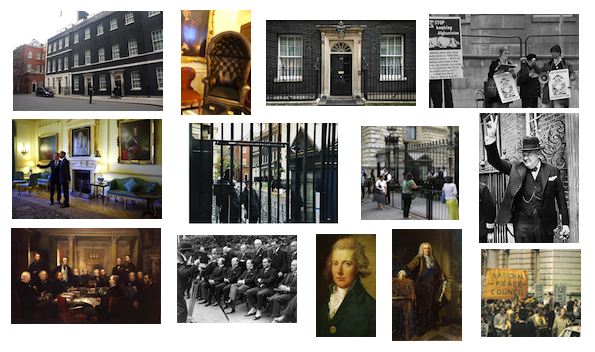
\includegraphics[width=0.9\textwidth]{images/10downingcollage.png}
\caption{A selection of images from Wikipedia for the object \lstinline!10_Downing_Street!.}
\label{fig:10downingcollage}
\end{figure}

WIthout more images of the same object, viewpoints, environmental conditions, objects of occlusion, and noise content of individual images may vary to such a large extent that an obvious match cannot be made. 

\section{Database Augmentation}

Existing work addresses this problem by including a process known as database augmentation, the background of which is given in Chapter~\ref{chpt:background}.

The database-side feature augmentation process of querying the baseline system with each model image creates what is known as an image graph -- the interconnection of matches between images. Each edge of the image graph infers that the two images connected share (at least part of) the same object. An image graph is not needed in this project, as the absolute ground-truth classes of each image are already known, and it is assumed that overlap between classes does not exist\footnote{This is a contentious point. See the footnote in Subsection~\ref{sub:performance}.}. In the dataset of model images used in this project, the lack of multiple images of the same object means that the amount of augmentation that occurs is negligible, so the gains of database-side spatial feature augmentation are non-existent.

\section{Turbo-boosting}

While database-side feature augmentation is not suited to this application, the overall idea of feature augmentation can still be used, with a process called \emph{turbo-boosting}. 

Turbo-boosting is the augmentation of features from images of a completely independent dataset. The process is exactly that of spatially verified database expansion \cite{rootsift12}, however rather than the model images being used for augmentation, labelled images from Microsoft's Bing image search are used. A number of images, called \emph{turbo images} are downloaded for each class, by issuing a query to the Bing search engine (see Section~\ref{sec:turboimages}). For example, the turbo images for the class \lstinline!Tower_Bridge! are shown in Figure~\ref{fig:turboturboimages}. For each model image, if a turbo image matches it, the visual words of the turbo image are projected onto the model image.


Take, for example, the image in Figure~\ref{fig:turbomodelimage} as the first model image to be turbo-boosted. Each turbo image is tested to see if it matches the model image. In this example, the turbo image in Figure~\ref{fig:turboturboimage} matches against the model image, with the match being shown in Figure~\ref{fig:turbomatch}. The matched region is the bounding rectangle of the spatially verified visual words, with a slight margin. \emph{All} of the visual words contained with the matched region of the turbo image are projected onto the model image, as in Figure~\ref{fig:turboaugment}. The model image has now been augmented with the visual words of the turbo image.

This is repeated for every turbo image, for each model image of each class. If no match can be reasonably made with a turbo image, no augmentation occurs and the process continues with trying the next turbo image.

Once the turbo-boosting for every model image in every class has completed, the weighted histograms and new turbo-boosted index is created, just as for the baseline system (see Section~\ref{sec:histograms}). Matching is then performed just as with the baseline system, except that the turbo-boosted index and visual word vectors are used.

Turbo-boosting can be thought of as expanding the information content of the ground-truth image database (the model images) using an external dataset. Each model image is turbo-boosted in turn, outputting a new, more informative model image, which is used in place of the original to create a turbo-boosted dataset.

\begin{figure}[htb]
\centering 
\subfloat[Model images]{\label{fig:turbomodelimages}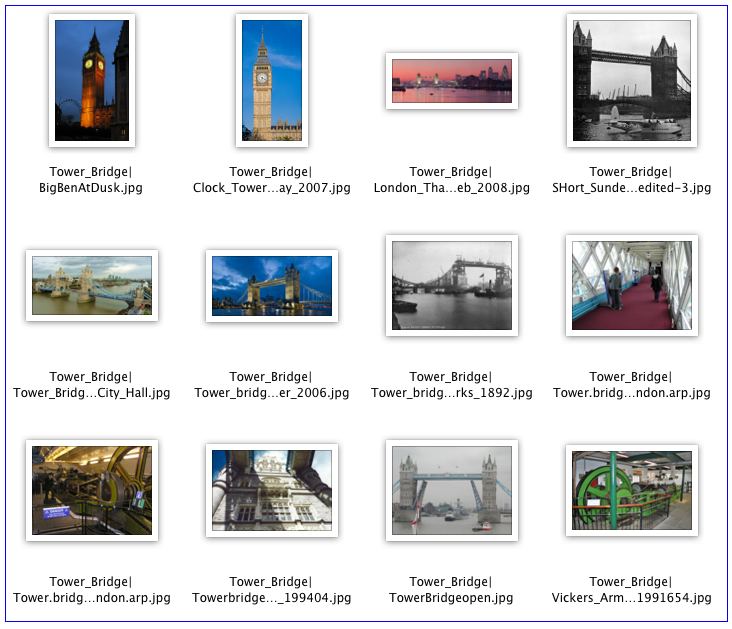
\includegraphics[width=0.35\textwidth]{images/wiki_tower_bridge.png}}
~
\subfloat[Turbo images]{\label{fig:turboturboimages}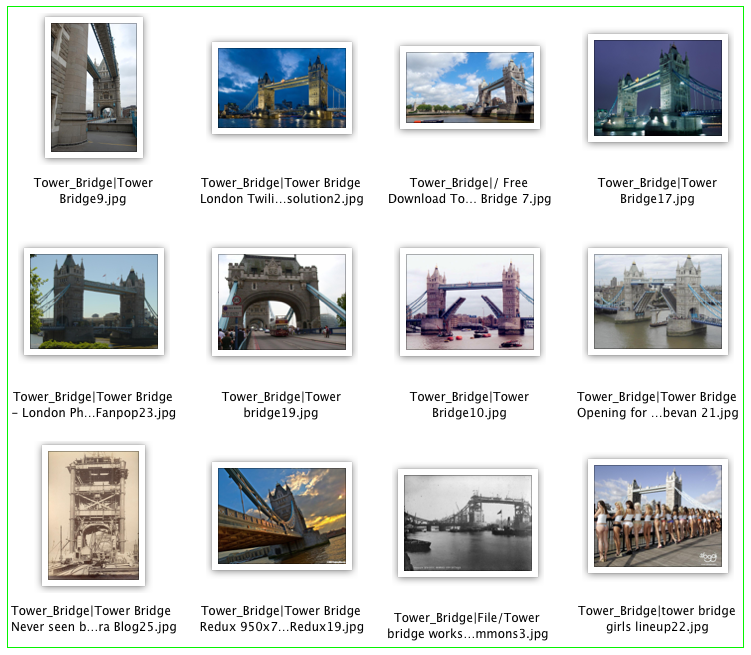
\includegraphics[width=0.35\textwidth]{images/bing_tower_bridge.png}}
\\
\subfloat[Model image words]{\label{fig:turbomodelimage}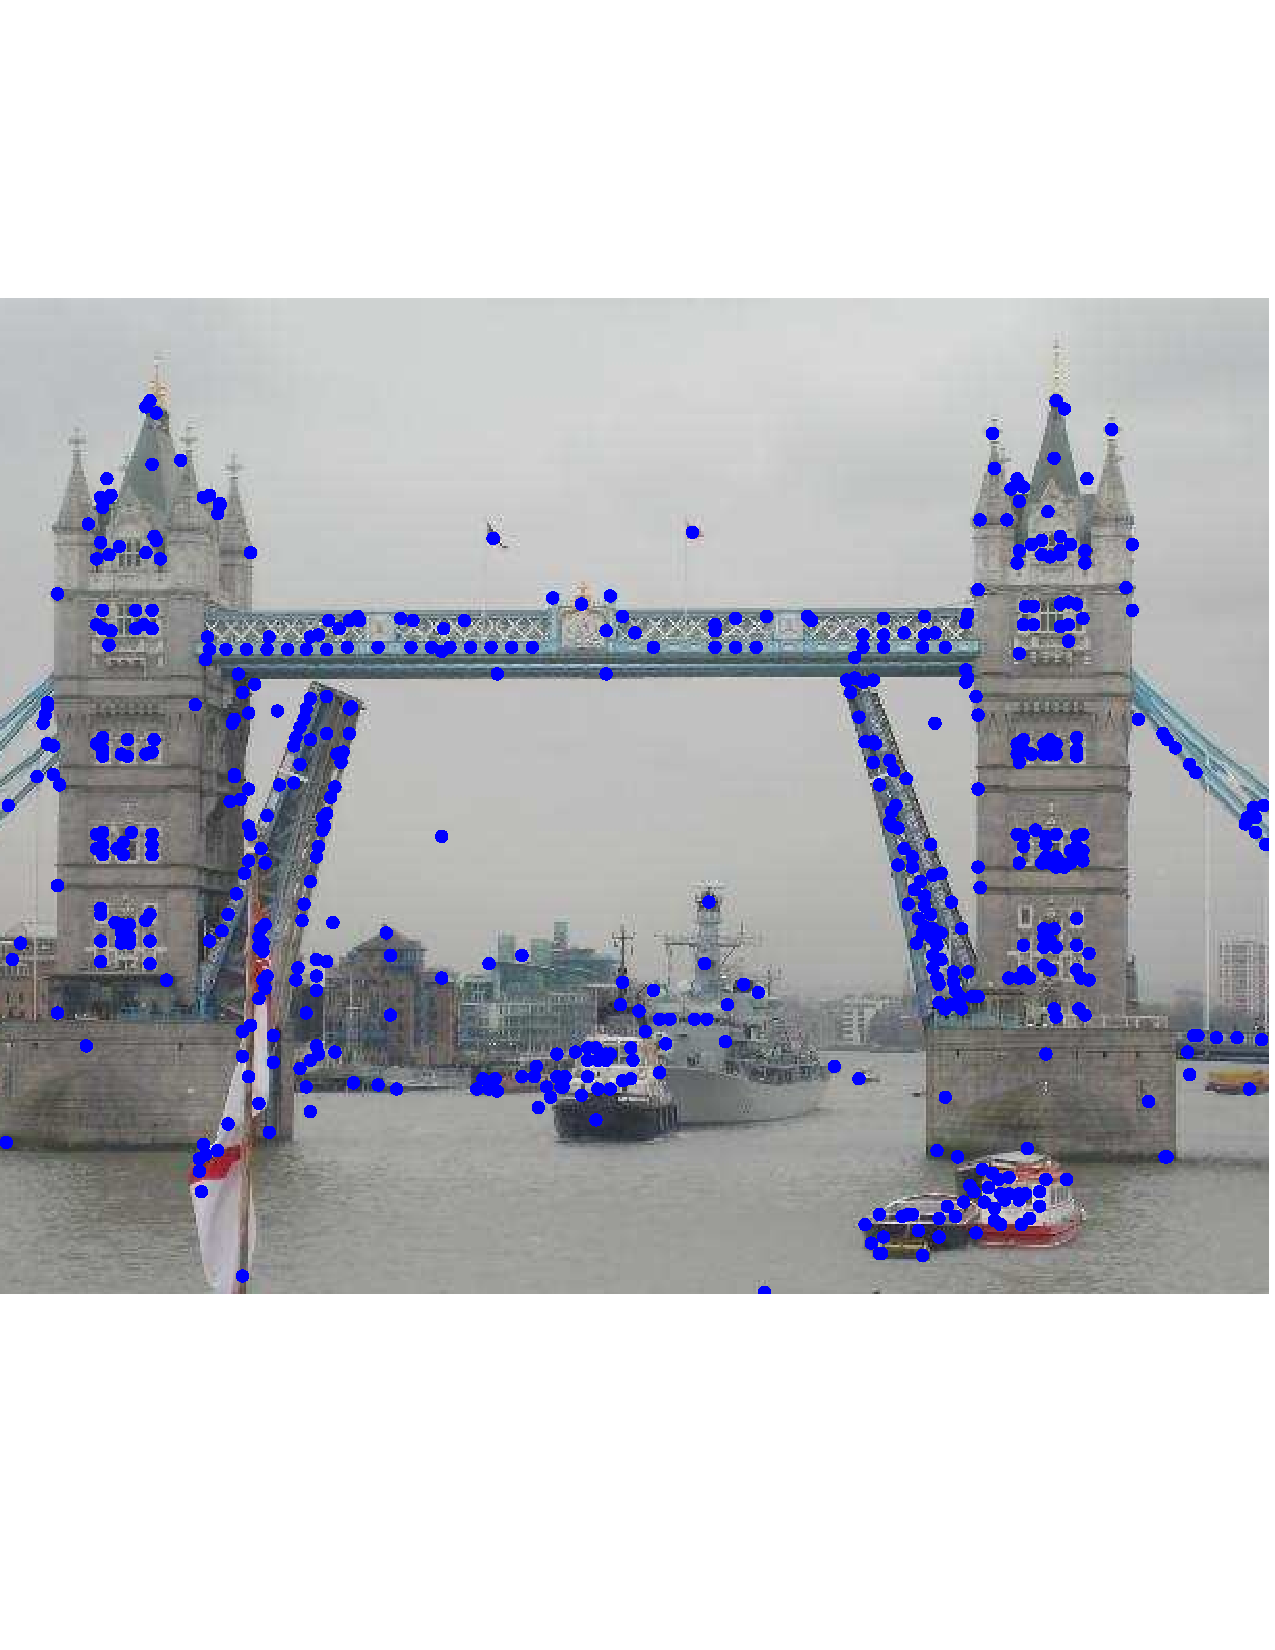
\includegraphics[width=0.35\textwidth]{images/c_im_words.pdf}}
~
\subfloat[Turbo image words]{\label{fig:turboturboimage}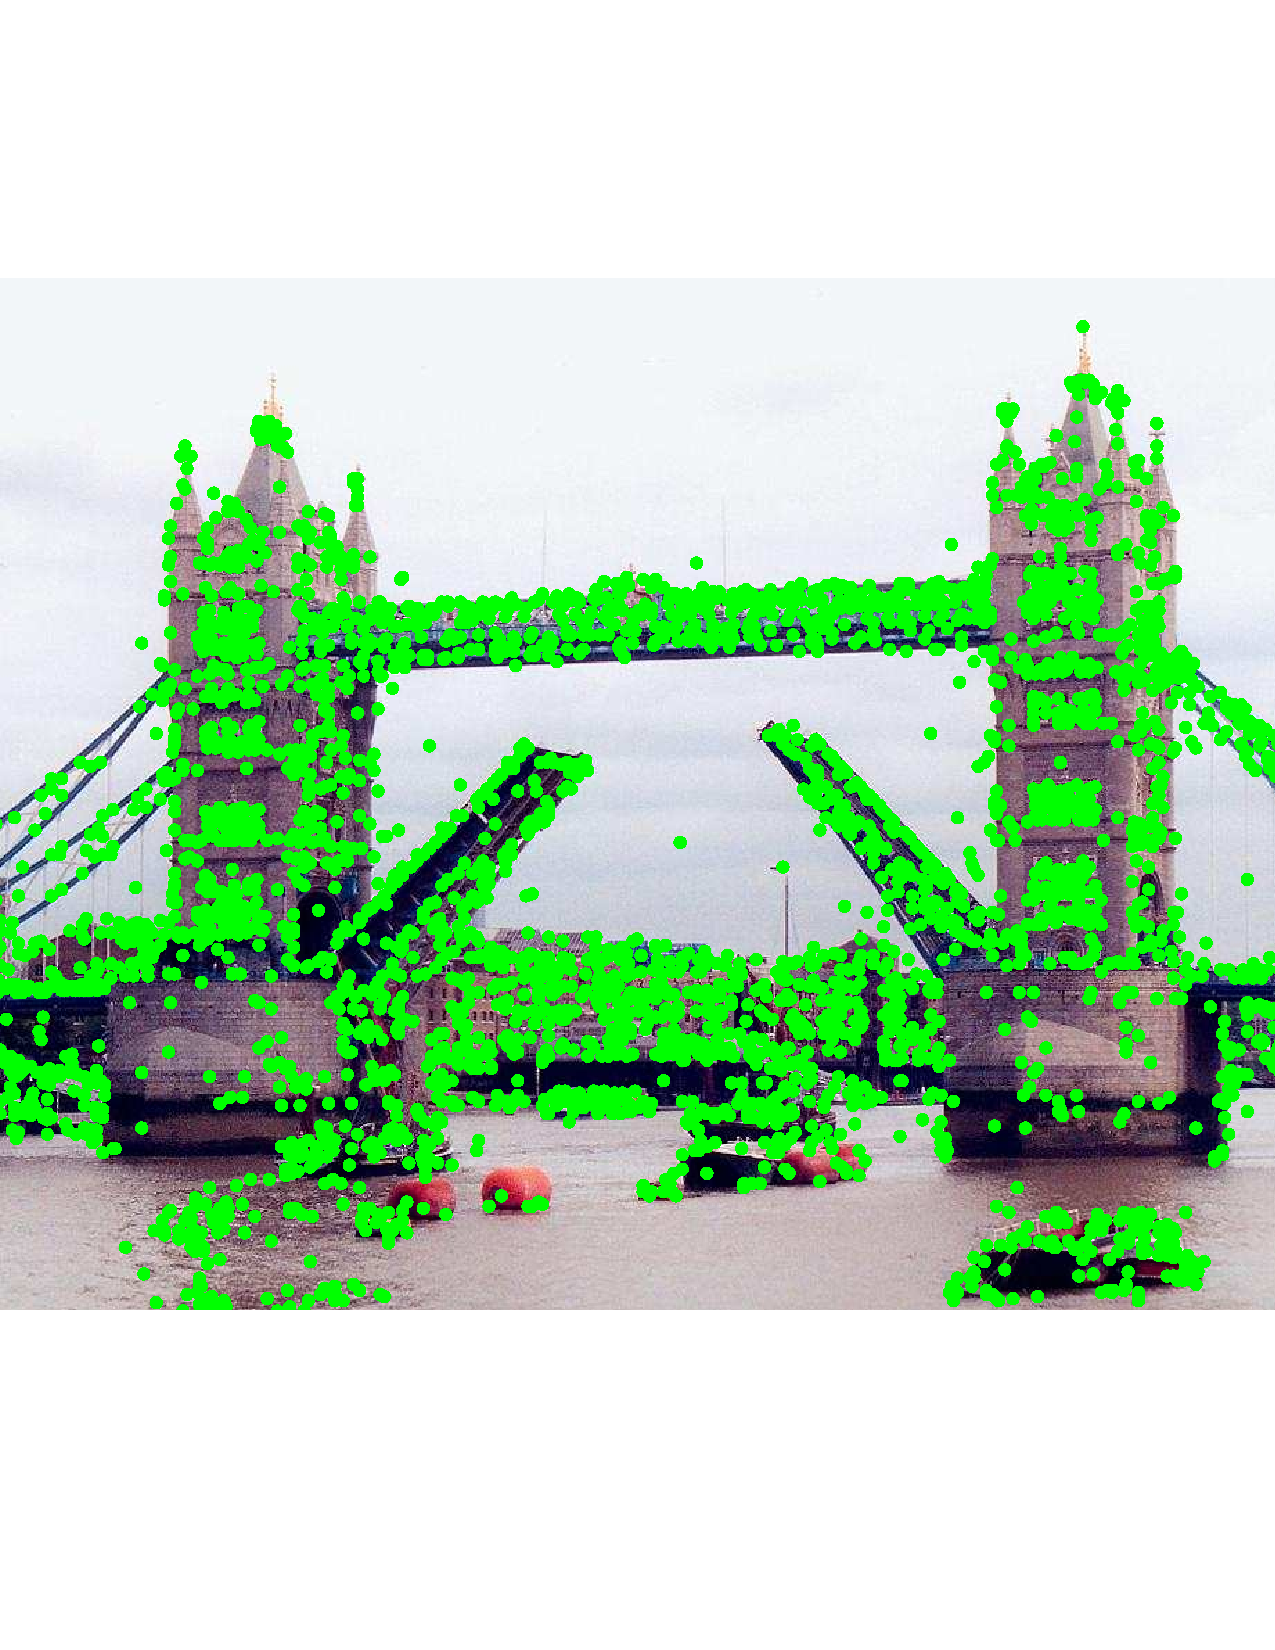
\includegraphics[width=0.35\textwidth]{images/f_im_words.pdf}}
\\
\subfloat[The turbo image is spatially verified with the model image]{\label{fig:turbomatch}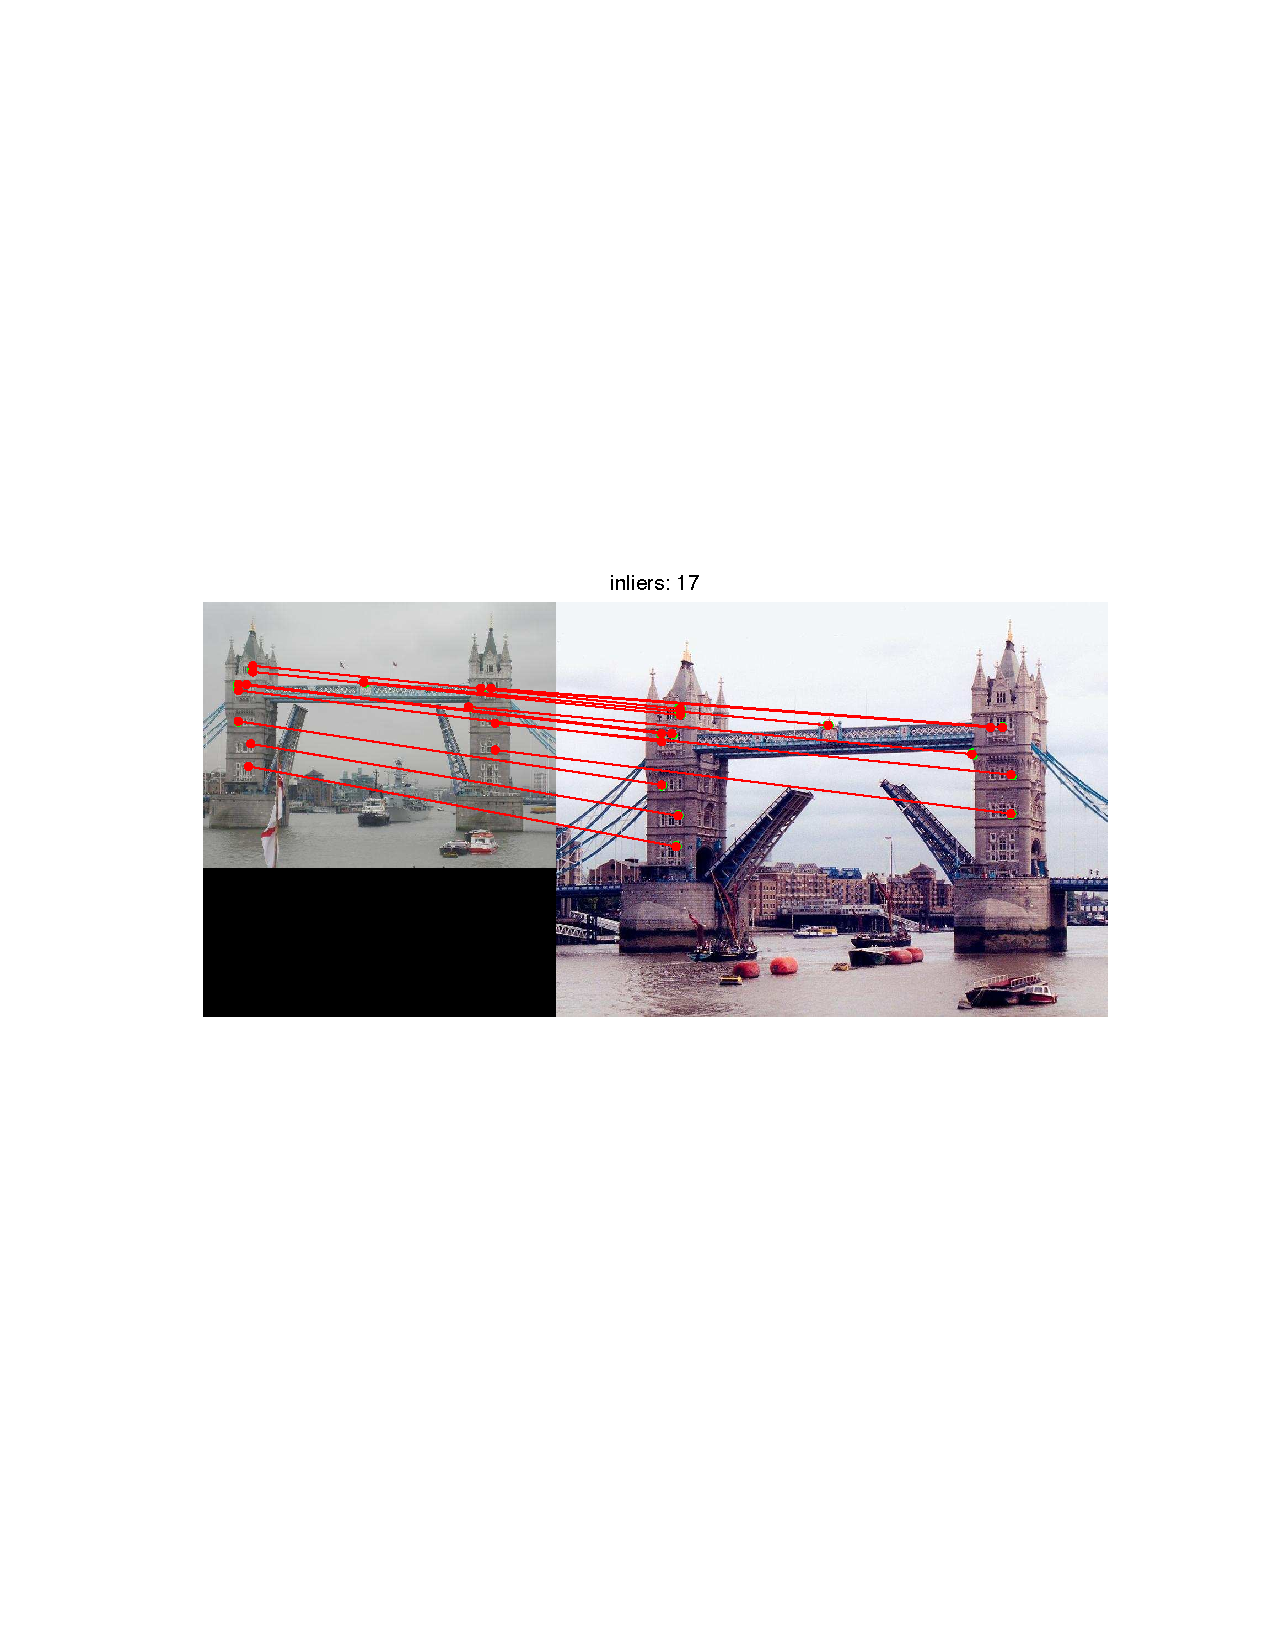
\includegraphics[width=0.7\textwidth]{images/tower_matches.pdf}}
\\
\subfloat[The words in the spatially verified region are used to augment the model image]{\label{fig:turboaugment}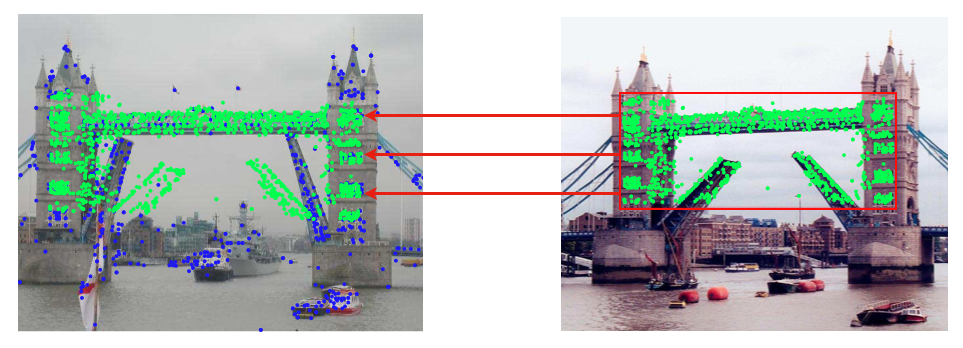
\includegraphics[width=0.7\textwidth]{images/augmentation.png}}
\caption{The turboboosting process.}
\label{fig:turboboosting}
\end{figure}

\clearpage


\section{Results and Analysis}

Including turbo-boosting in the pre-computation process dramatically increases the yield performance of the object recognition system. Table~\ref{tbl:turboresults} shows the yield performance of the system when turbo-boosting was included. The number of turbo images that are downloaded was varied. The results (shown in Table~\ref{tbl:turboresults} and Figure~\ref{fig:turbograph}) show that increasing the number of turbo images downloaded increases the yield, however this effect flattens out above 25 images. This is because downloading additional turbo images will not bring in many new features to augment the model images -- the model images become saturated with data.

\begin{table}[hbtp]
\begin{center}
\begin{tabular}{c|c|c|c|c|c|c|c|}
\cline{2-8}
 & \multicolumn{7}{|c|}{\# Turbo images downloaded} \\ 
 \cline{2-8}
 & 0 & 5 & 10 & 15 & 25 & 35 & 50 \\
 \cline{2-8}
 \cline{1-8}
\multicolumn{1}{|c||}{Yield} & \texttt{22.6\%} & \texttt{25.2\%} & \texttt{26.1\%} & \texttt{27.8\%} & \texttt{31.1\%} & \texttt{31.2\%} & \textcolor{red}{\texttt{31.7\%}}\\
\cline{1-8}
\end{tabular}
\end{center}
\caption{The yields achieved using different levels of turbo-boosting with the Affine RootSIFT configuration and an inlier threshold of 5.}
\label{tbl:turboresults}
\end{table}
 

Overall, turbo-boosting increases the performance by 75\% with respect to the baseline system, and 29\% compared to the best possible configurations without turbo-boosting.

\begin{figure}[hbtp]
\centering 
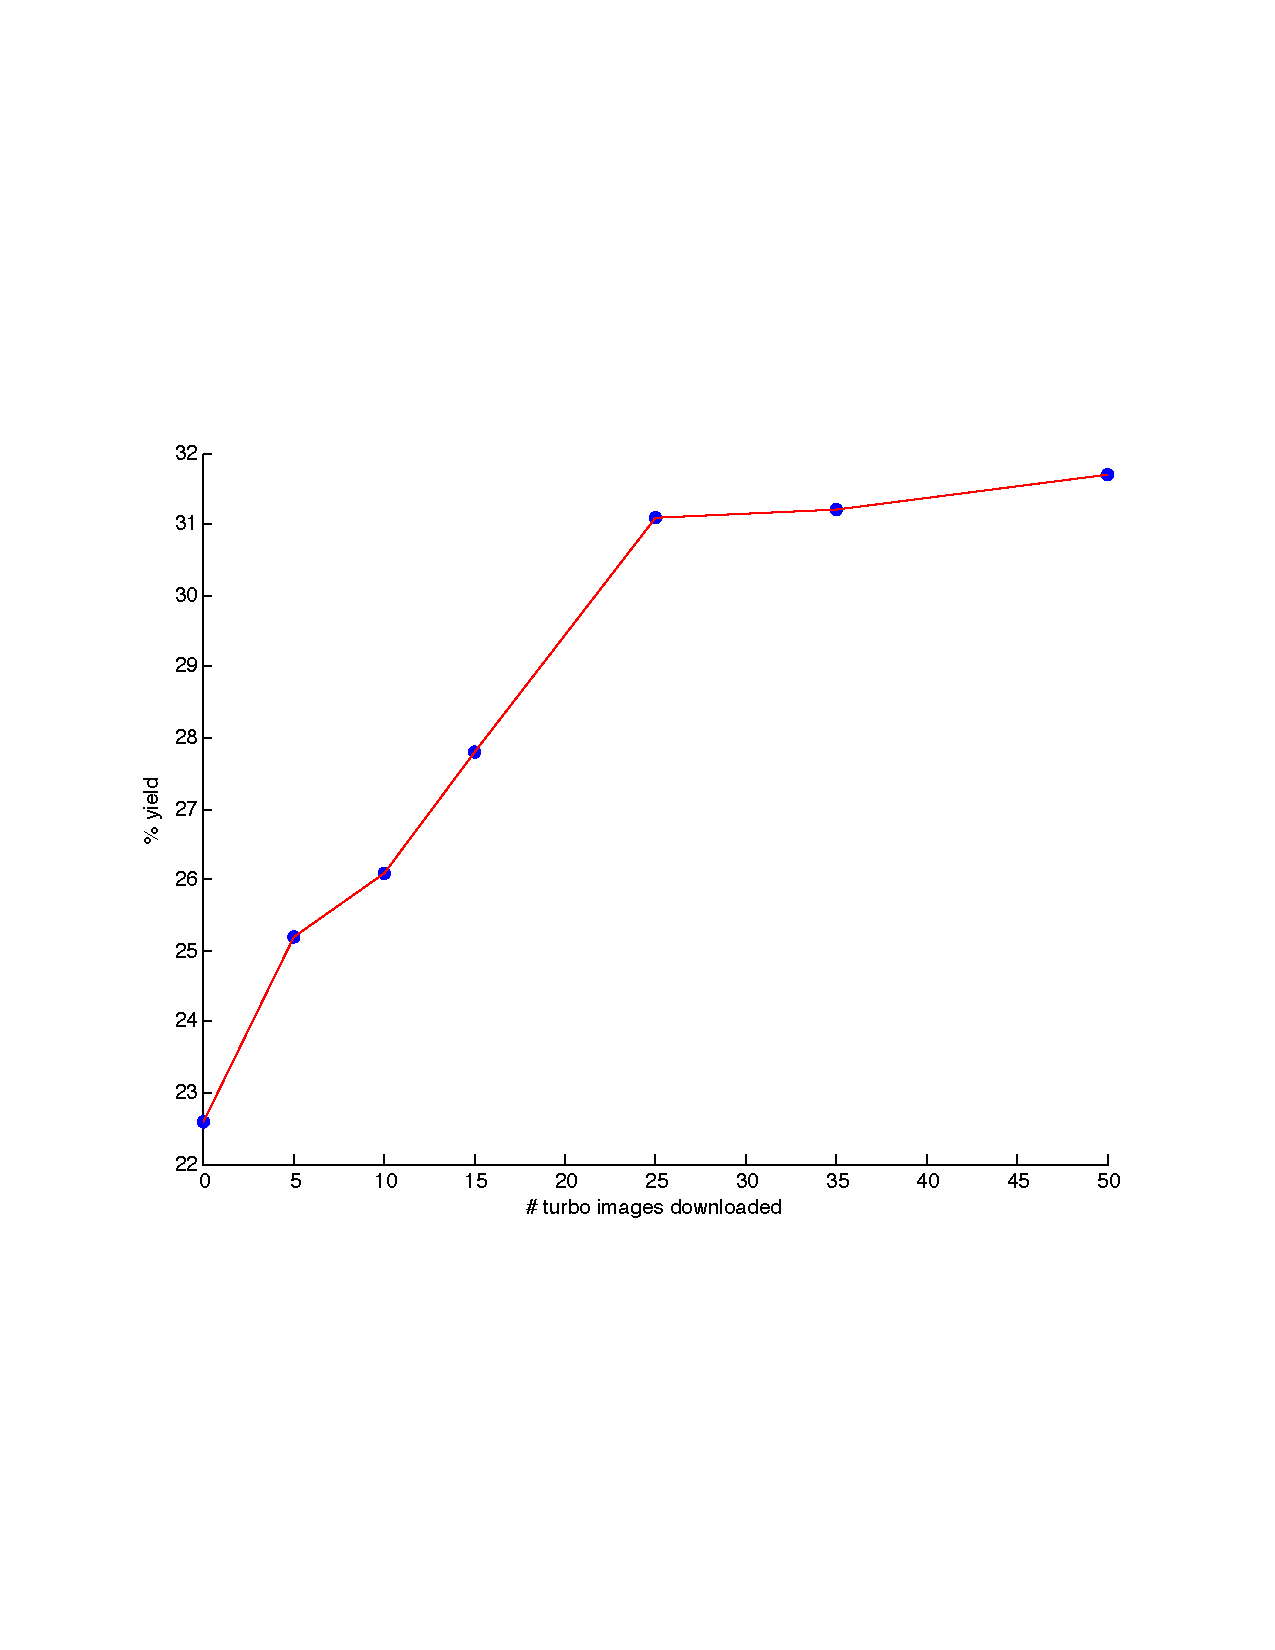
\includegraphics[width=0.5\textwidth]{images/turbograph.pdf}
\caption{The effect on yield by increasing the number of turbo images downloaded.}
\label{fig:turbograph}
\end{figure}

Turbo-boosting works by increasing the information content of the model images. When a turbo image is spatially verified with a model image, it may be verified on a minimum of seven visual words. However, many hundreds of words can be added to the model image's visual word vector, as all the words contained within the bounding box of the few spatially verified visual words are added. These added words help matching in three ways:

\begin{itemize}
\item There may be features that were detected in the turbo image that were not detected in the model image. When these visual words are added to the model image from turbo-boosting, this creates a more detailed description of the object in the model image.
\item Some features common to both images may be described by different visual words due to noise. After turbo-boosting, both visual words will therefore be in the same position in the model image describing the same feature. This increases the robustness to noise.
\item Some augmented features will be duplicates -- a duplicate feature being one that is common to both the turbo image and the model image and is described by the same visual word in both cases. This means that after turbo-boosting, the model image will contain  multiple identical visual words for the same feature. This effectively gives the feature more weight for matching.
\end{itemize}

Figure~\ref{fig:turboresult} shows a case where the query image Figure~\ref{fig:turboresultqueryimage} cannot be matched to any model images. The inlier threshold is set to 5 so the model image, Figure~\ref{fig:turboresultmodelimage}, does not match with the query image, as there are only 4 inliers (Figure~\ref{fig:turboresultvanilla}). However, the model image  can be turbo-boosted (due to the match in Figure~\ref{fig:turboresultturbomatch}), leading to the augmentation of the words in the matched region of the turbo image Figure~\ref{fig:turboresultturboimage}. The turbo-boosted model image now matches against the query, as shown in Figure~\ref{fig:turboresultturbo}. There are many examples of cases similar to this one -- where the model image is perfectly representative of the object, but does not have enough stable visual words to match reliably. However, due to the large number of turbo images, some augmentation occurs which pulls in better stable visual words.

%temple bar london is a good example

There are cases where turbo-boosting makes no difference to the recognition of an object. This is mainly due to there being no turbo images which match to the model images, so no augmentation occurs. This is an issue which is unavoidable due to low number of representative model images for some objects. 

Turbo-boosting is a completely general strategy for increasing the yield/recall -- any labelled dataset can use this technique. The only draw backs are the increase in pre-computation time due to the turbo-boosting routine, which is $O(N_c\overline{N}_mN_t)$ where $N_c$ is the number of classes, $\overline{N}_m$ is the average number of model images of each class, and $N_t$ is the number of turbo images that are downloaded. The increase in pre-computation time can be overcome as the process is easily parallelised -- the inner loop on each class is completely independent. Another disadvantage is the slight increase in storage needed. The downloaded turbo images can be deleted as they are only needed temporarily, however due to the increase of visual words in each model's vector and the fact that the histograms will be generally less sparse after augmentation, the byte size of these structures increases.

\begin{figure}[t!]
\centering 
\subfloat[Query image]{\label{fig:turboresultqueryimage}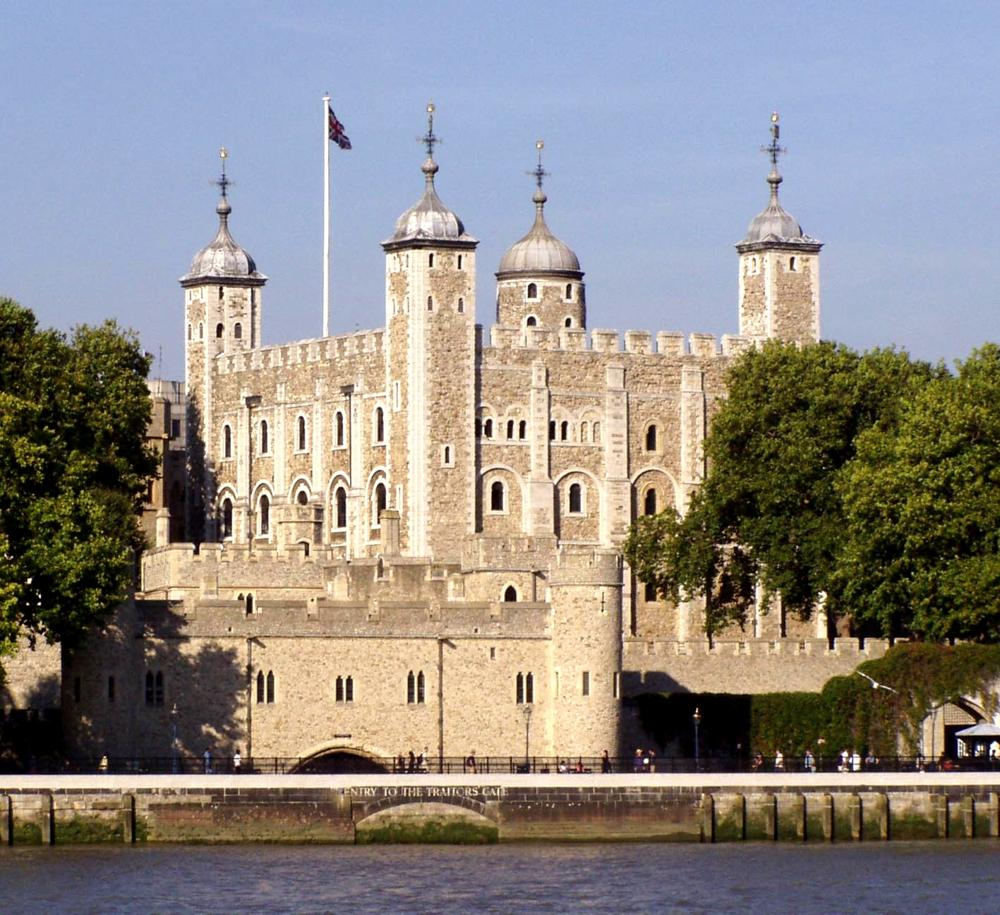
\includegraphics[width=0.25\textwidth]{images/turboquery.jpg}}
~
\subfloat[Model image]{\label{fig:turboresultmodelimage}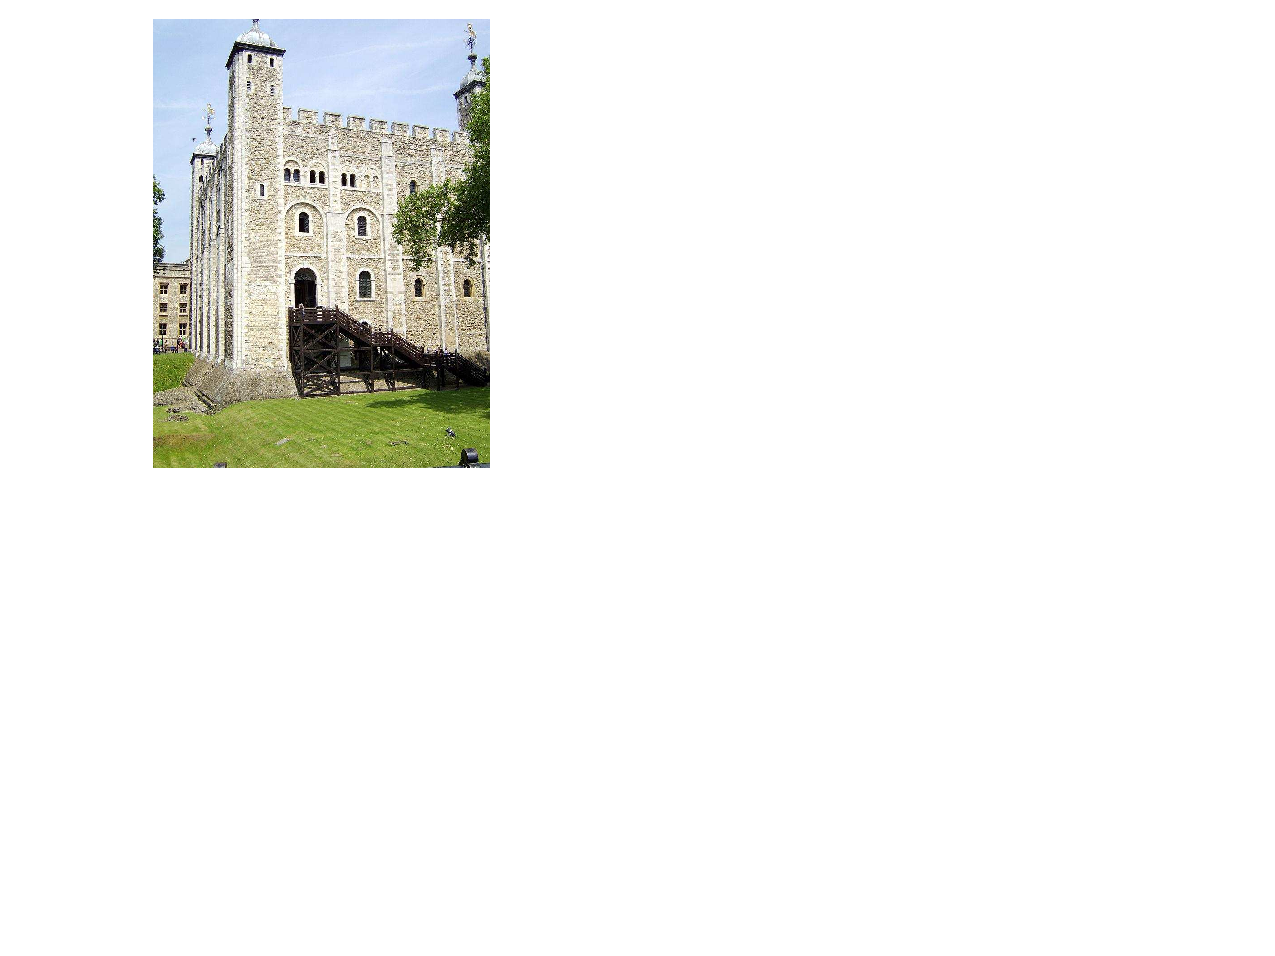
\includegraphics[width=0.2\textwidth]{images/turbomodelimage.pdf}}
~
\subfloat[Turbo image]{\label{fig:turboresultturboimage}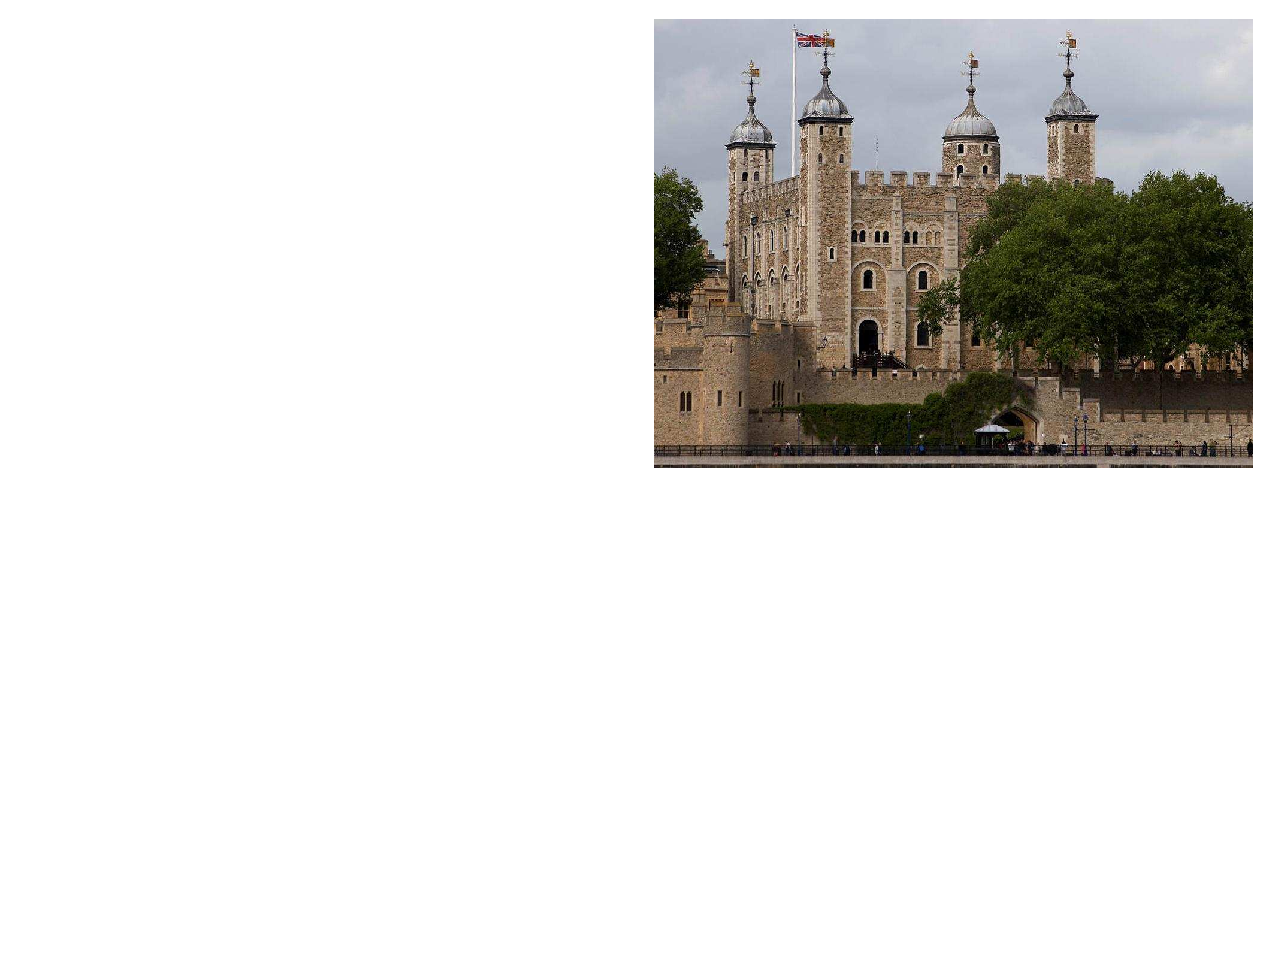
\includegraphics[width=0.25\textwidth]{images/turbomatch.pdf}}
\\
\subfloat[The match before turbo-boosting]{\label{fig:turboresultvanilla}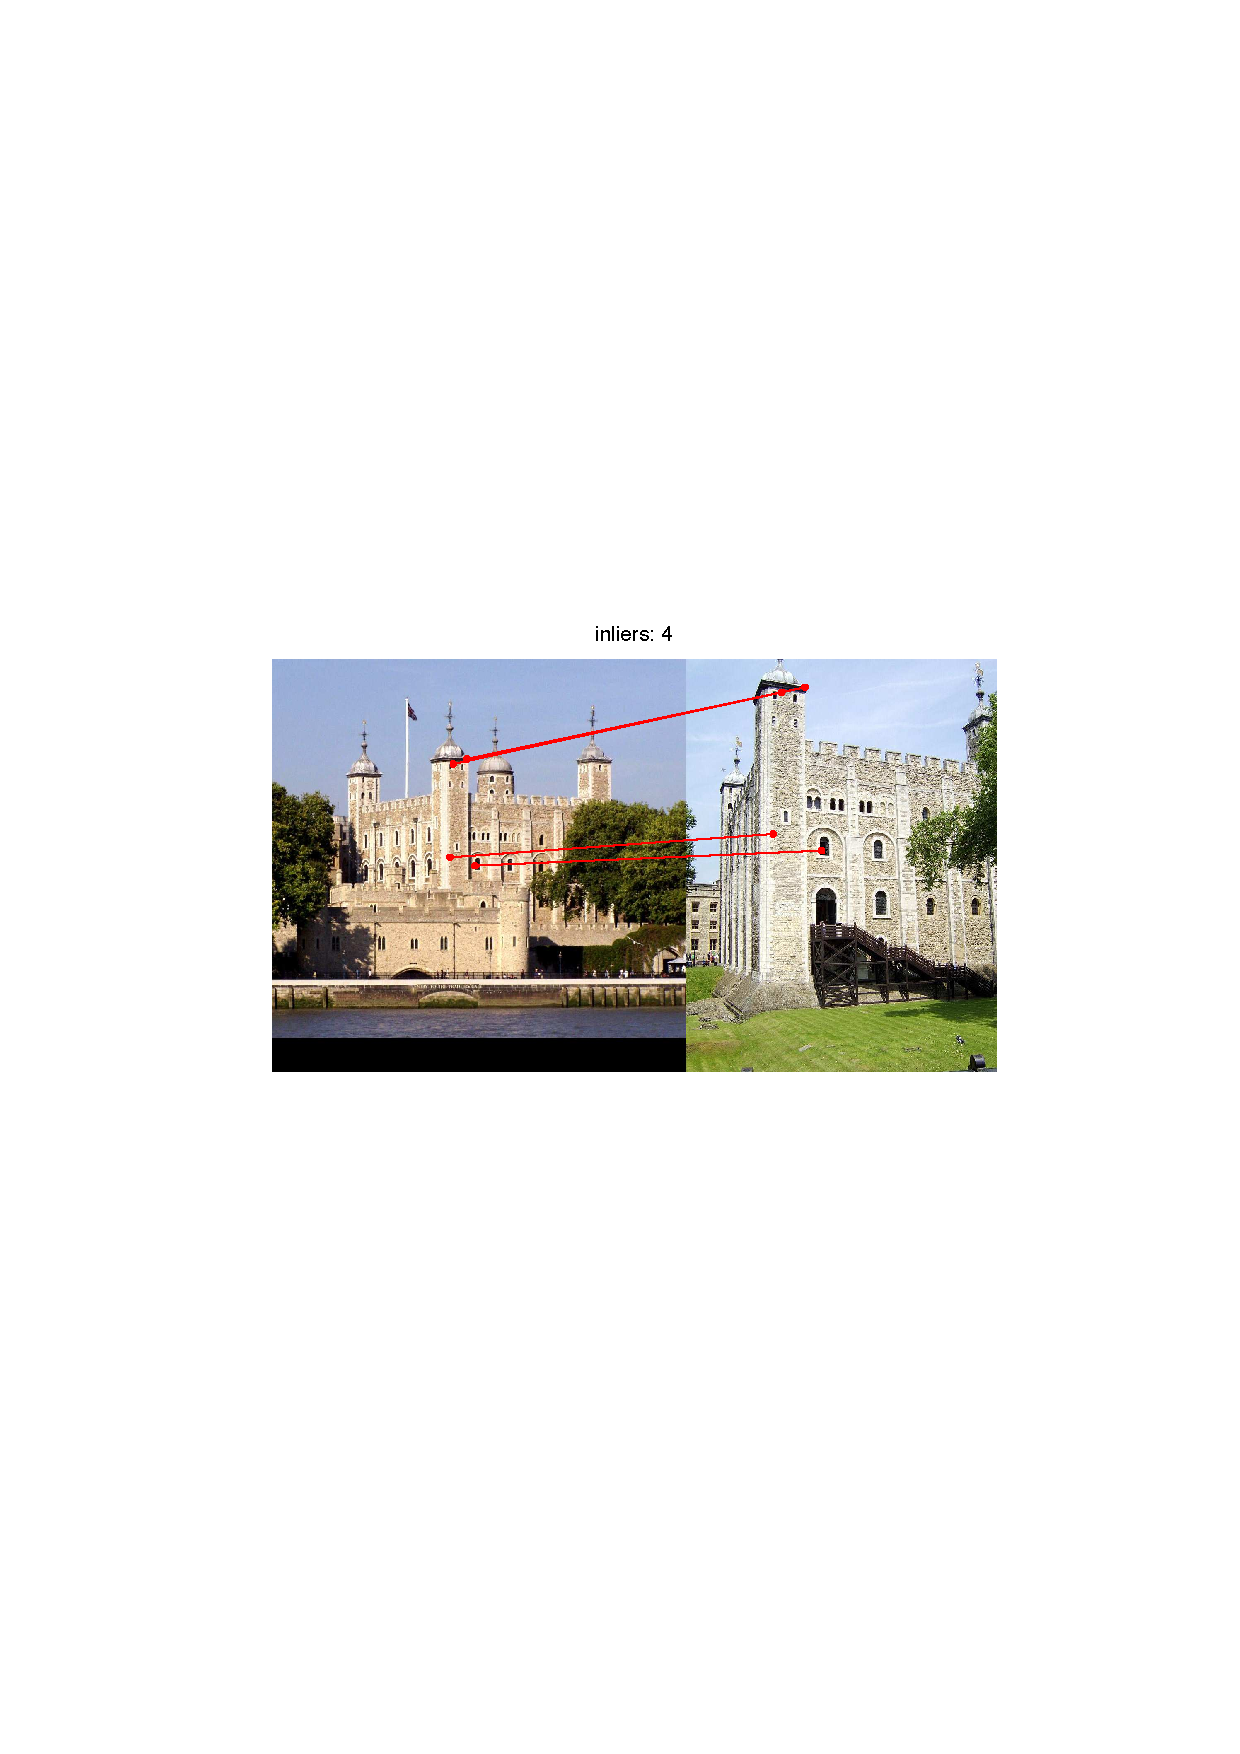
\includegraphics[width=0.45\textwidth]{images/query_vanillamodel.pdf}}
~
\subfloat[The turbo image matching the model image]{\label{fig:turboresultturbomatch}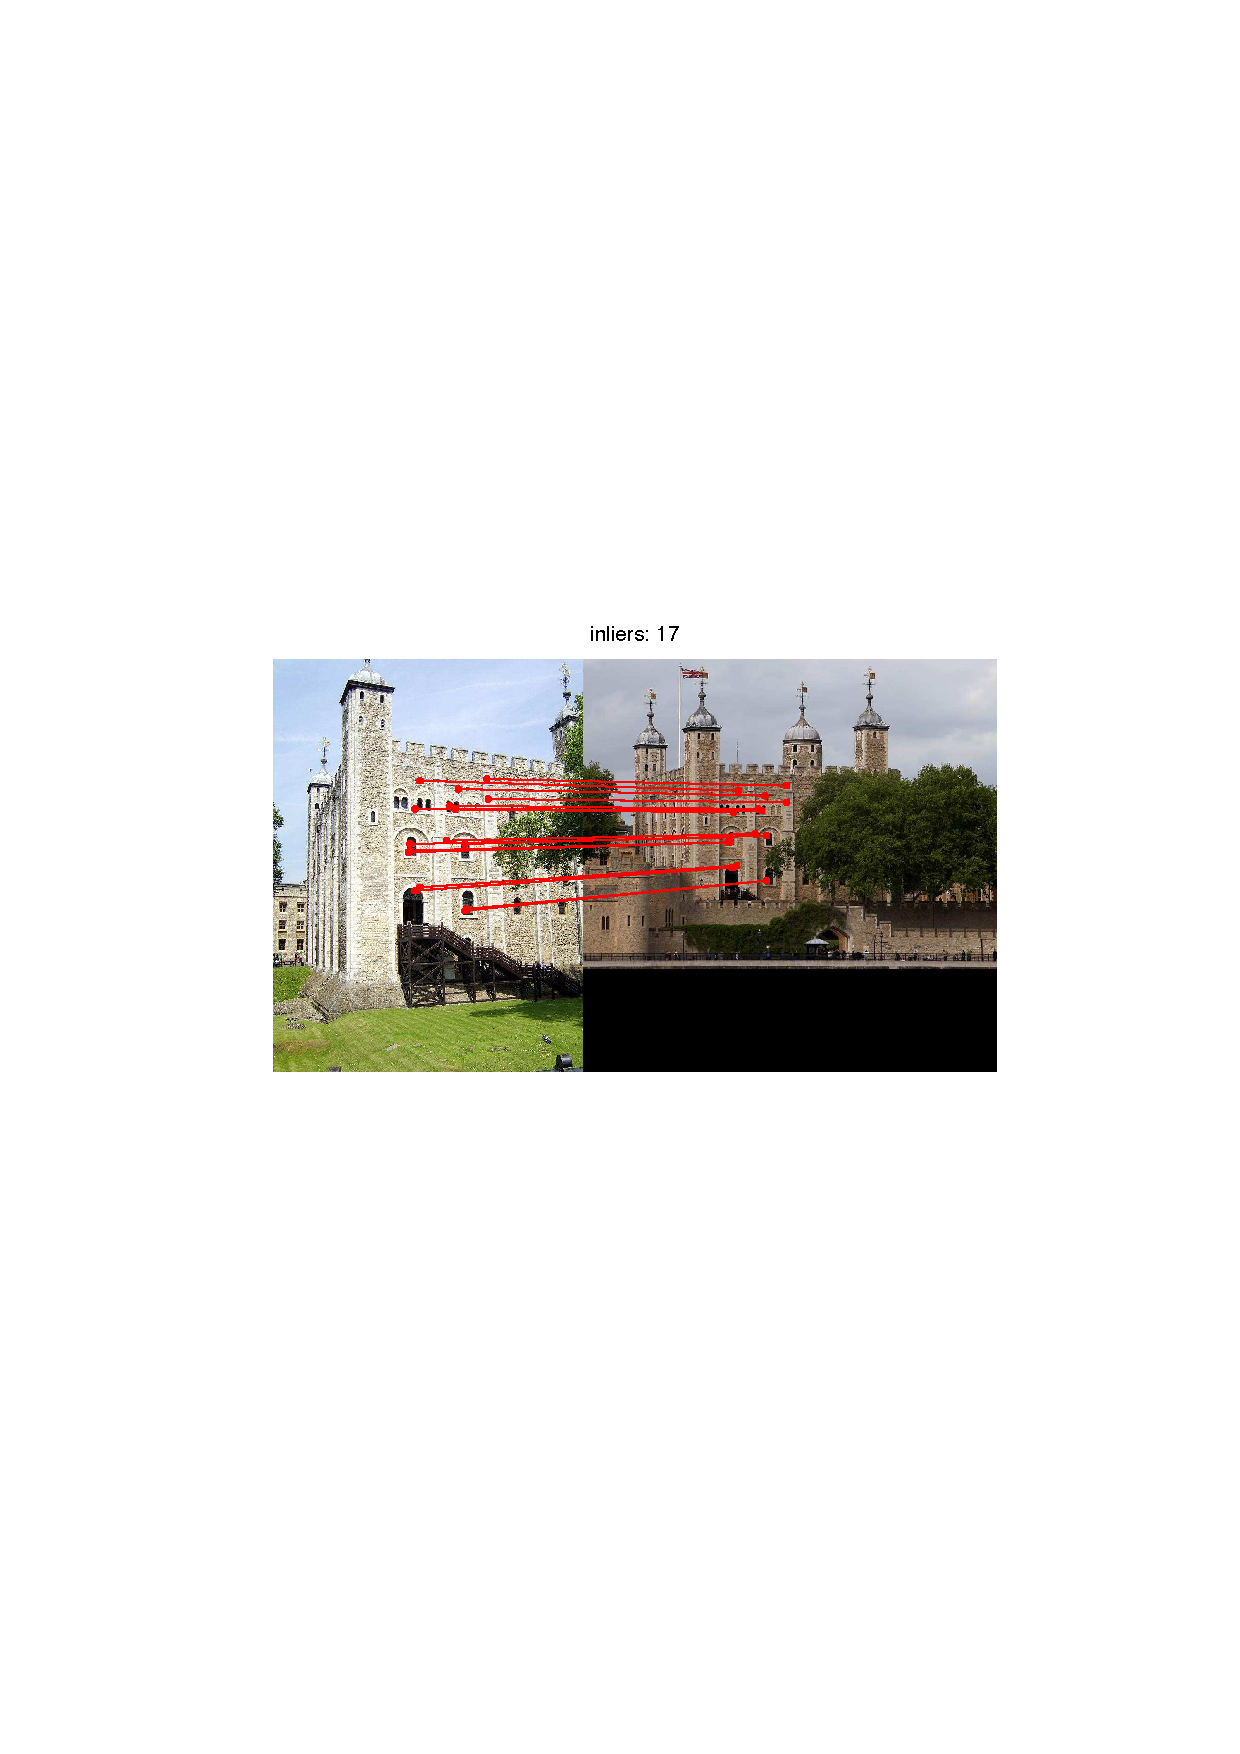
\includegraphics[width=0.45\textwidth]{images/model_turbo.pdf}}
\\
\subfloat[The match after turbo-boosting]{\label{fig:turboresultturbo}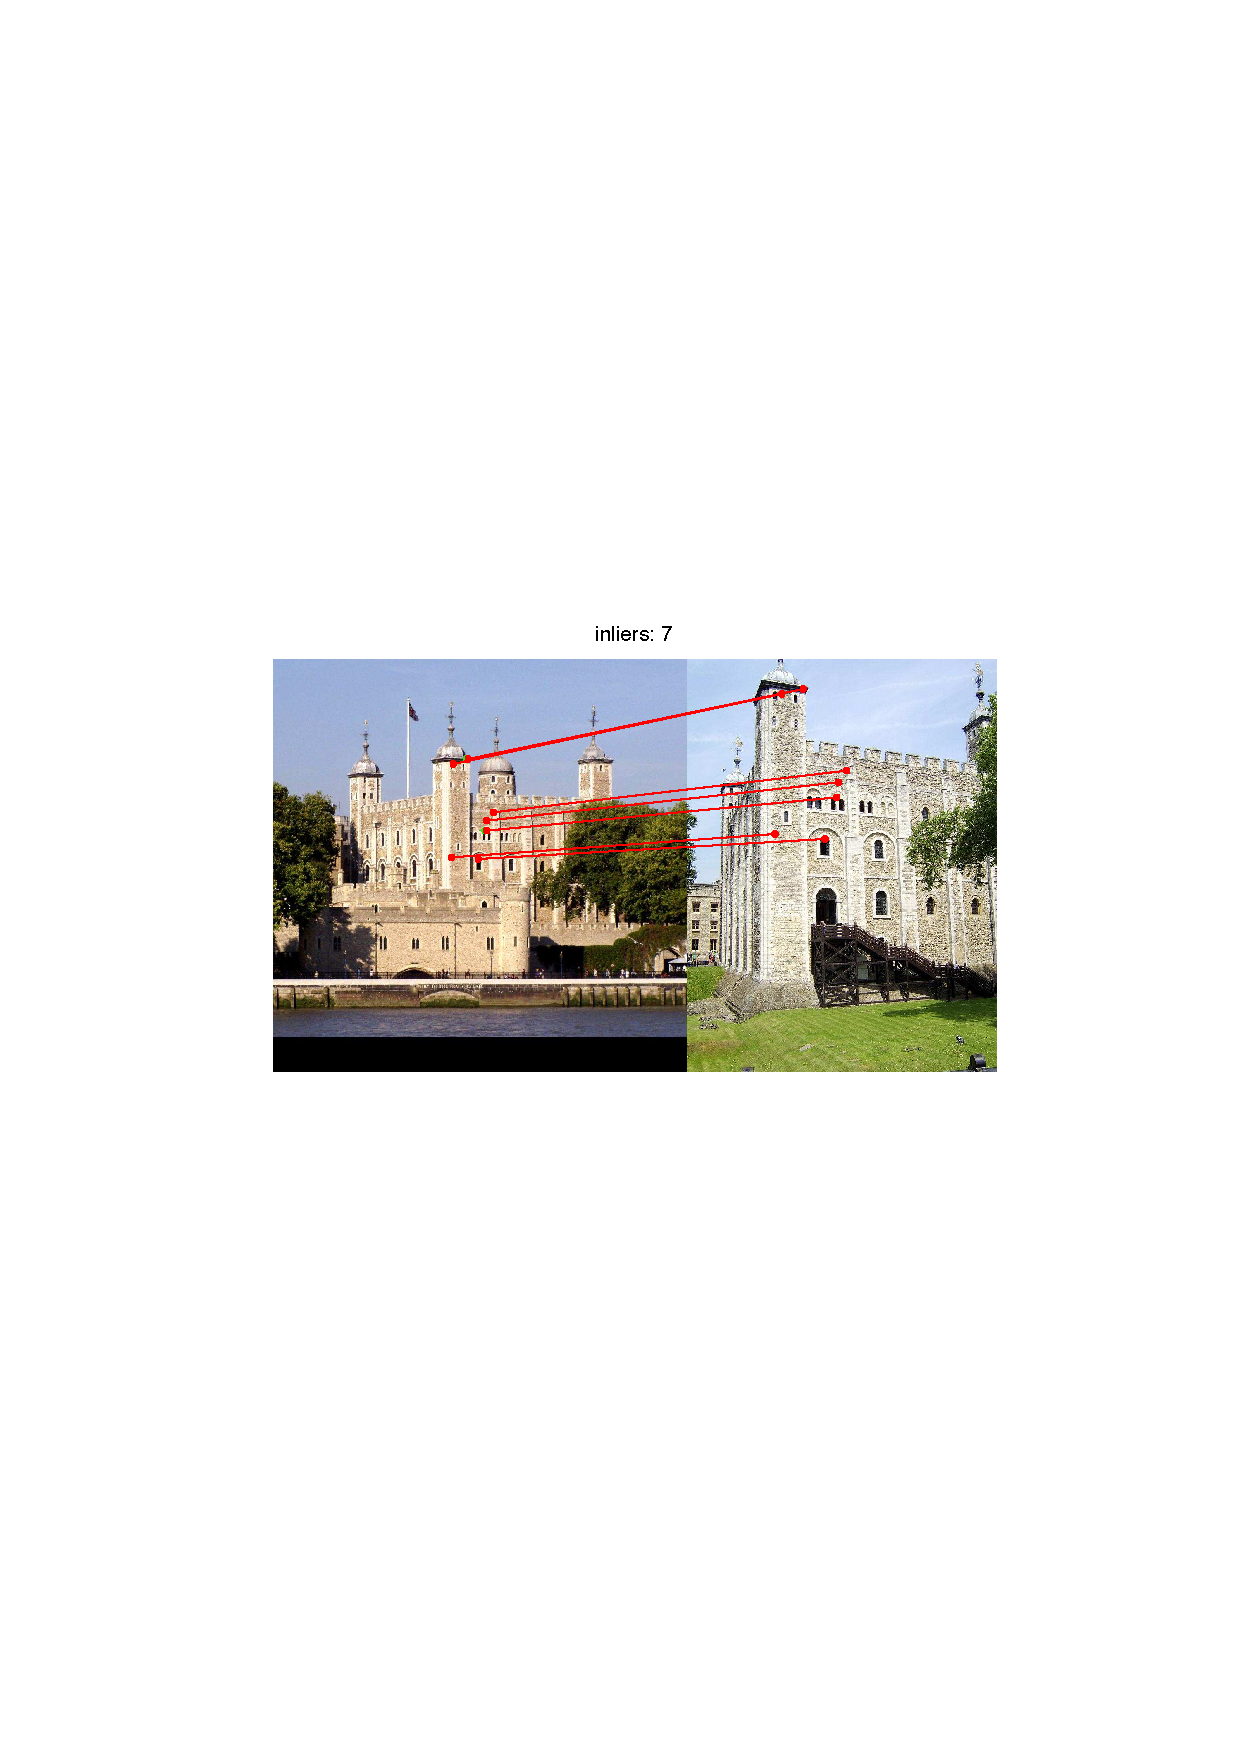
\includegraphics[width=0.5\textwidth]{images/query_turbomodel.pdf}}

\caption{The query image Figure~\ref{fig:turboresultqueryimage} will not be identified unless model image Figure~\ref{fig:turboresultmodelimage} is augmented with the words of Figure~\ref{fig:turboresultturboimage}.}
\label{fig:turboresult}
\end{figure}

%-------------------------------
% Implementation
%-------------------------------
\linespread{1}\chapter{Implementation}
\label{chpt:architecture}
While Chapter~\ref{chpt:system} outlines the processes involved with the object recognition engine, this chapter describes the practical implementation of the system including the front end web application for consumer interaction.

\begin{figure}[htb]
\centering 
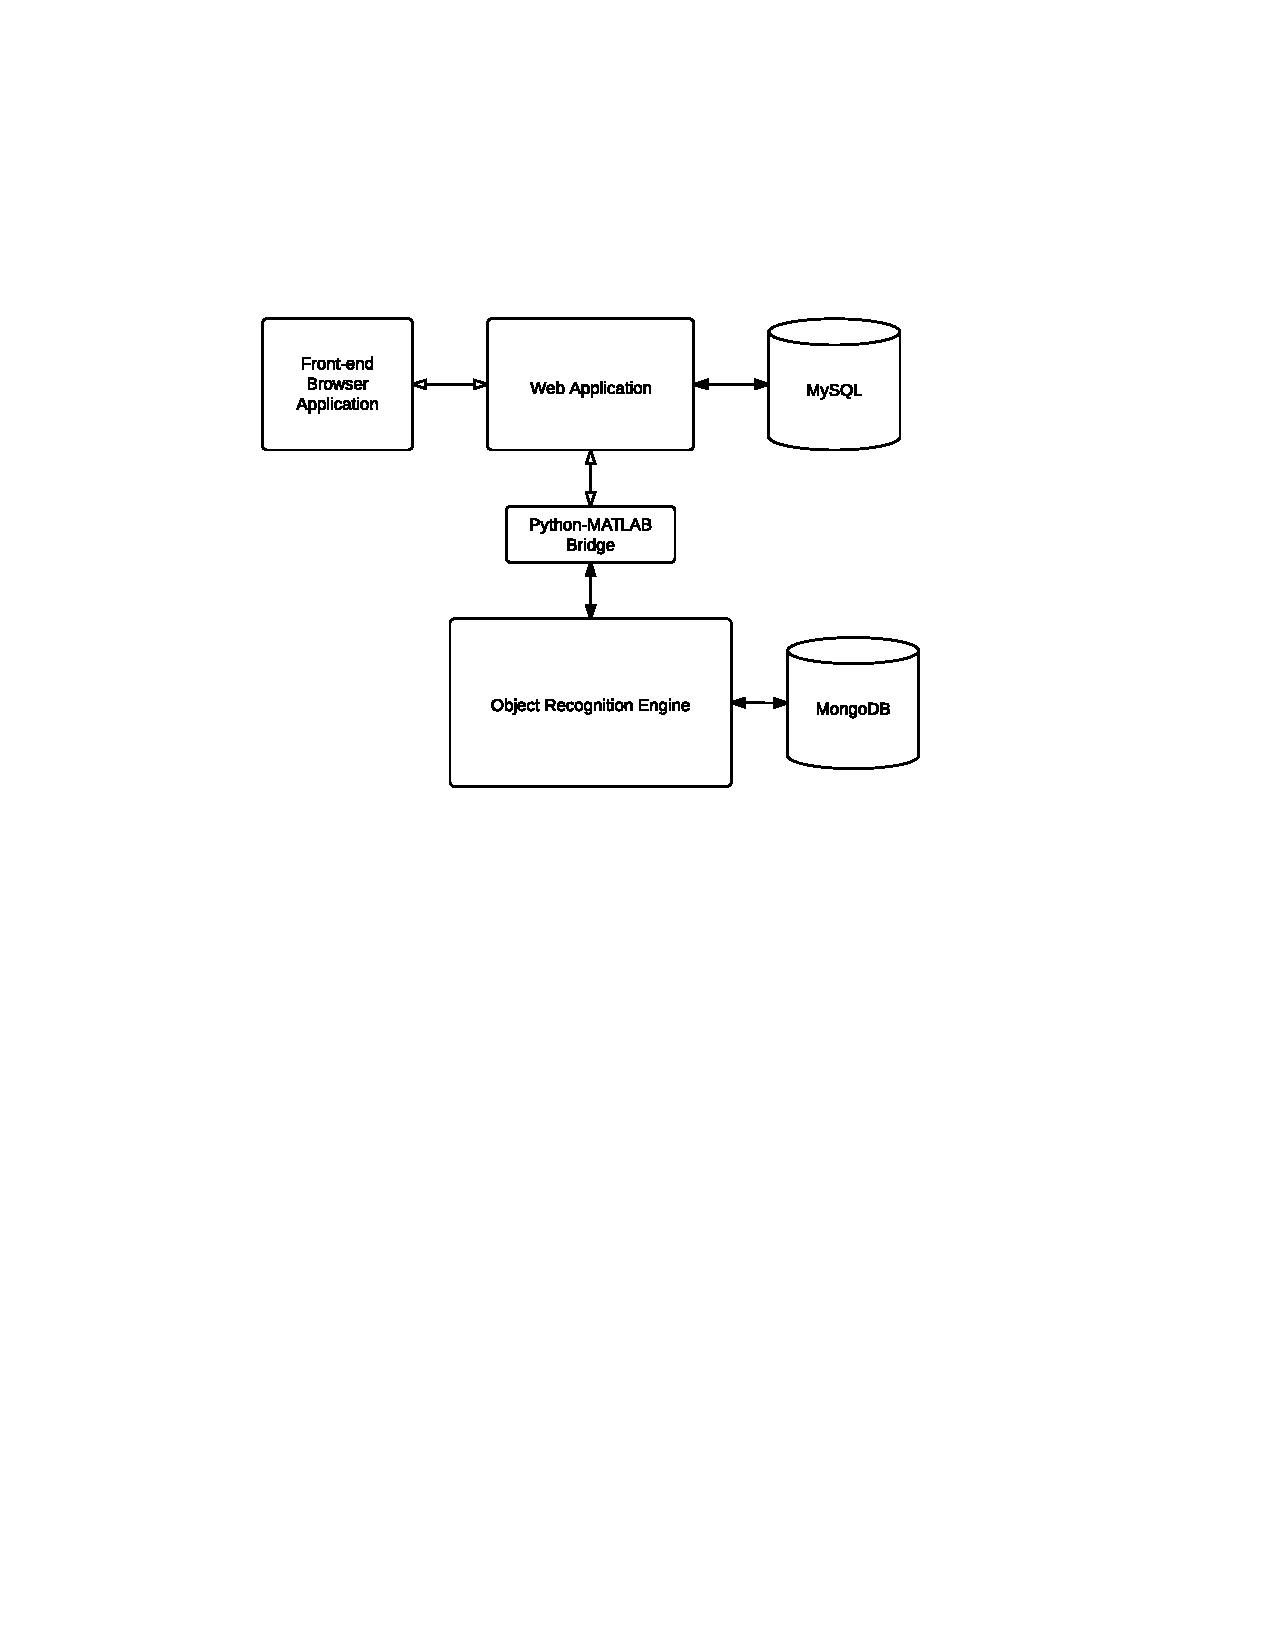
\includegraphics[width=0.5\textwidth]{images/SystemArchitecture.pdf}
\caption{An overview of the system architecture.}
\label{fig:architecture}
\end{figure}

Figure~\ref{fig:architecture} gives a holistic view of the system architecture. The solution is divided in to two separate parts: the object recognition engine and the web application. These are described in Section~\ref{sec:engine} and Section~\ref{sec:webapp} respectively. These two parts are completely independent modules by design, however they are connected via a Python-MATLAB bridge, the details of which are given in Section~\ref{sec:bridge}.

The resulting product is a web site with an intuitive user interface. A user can upload a photo, and the photo will be presented back to the user with the objects tagged.

\section{Object Recognition Engine}
\label{sec:engine}
The object recognition engine performs the pre-computation and recognition processes described in Chapter~\ref{chpt:system}. This is all implemented using MATLAB. MATLAB was chosen due to its ease in image manipulation, rich toolboxes, and the provided starter application was written in MATLAB.

The resulting interface is a MATLAB function \lstinline!get_objects()! that takes a single argument containing the location of the query image to recognise the objects in. The output is a structure of the object classes found and their bounding rectangles in the query image. The function takes around 5-10 seconds to run.

\subsection{Database}

A filesystem is used for the storage of model images (see Chapter~\ref{chpt:data}), however a working record is needed of the dataset for book keeping and quick searching. For this, MongoDB\footnote{\url{http://www.mongodb.org}} is used. 

MongoDB is a NoSQL\footnote{NoSQL is a family of databases that does not require fixed table schemas, and are sometimes known as ``structured storage''.} database application that stores data in the form of documents -- data structures similar to JSON objects. The data is unstructured, and provides a simple way of storing data without dealing with the complexities of tables and relationships that come with relational databases (e.g. SQL). Listing~\ref{lst:bson} shows a model image stored in the MongoDB database. The fields of the documents (i.e. \lstinline!"_id", "name", "path", "class", "size"!) are fully searchable and can be indexed for faster lookup\footnote{By deafault, the \lstinline!"_id"! field is indexed for fast lookup by ID.}. 


\linespread{1} % single line spacing
\lstset{language=Java,caption=A document representing a model image stored in MongoDB.,label=lst:bson}
\begin{lstlisting}[frame=single]
// BSON
{
	"_id" : ObjectId("4f7317501b515eaa6f148c5d"),
	"name" : "1222|10_Downing_Street.jpg",
	"path" : "~/4YP/data/d_ransac/images/10_Downing_Street/1222|10_Downing_Street.jpg",
	"class" : "10_Downing_Street",
	"size" : {
		"width" : 800,
		"height" : 457
	}
}
\end{lstlisting}
\linespread{2} % double line spacing

MongoDB is run as a daemon and the location of the database's files is set to be a directory within the solution's working directory. This allows complete segmentation of each database. The daemon sets up a web server on port \lstinline!3036! which can accept any number of connections over TCP to access the database.

The interface with MATLAB is done using the Java library provided by MongoDB\footnote{See \url{http://www.mongodb.org/display/DOCS/Java+Tutorial} for documentation.}. MATLAB has the ability to run Java inside it, so the Java MongoDB library can be consumed in a fairly natural way.

The frames, descriptors, words and histograms for the model images are stored on disk as MATLAB binary files. They are associated to the database entries via their filename which includes the ID assigned by MongoDB to the image's document. For example, for the model image \lstinline!1222|10_Downing_Street.jpg! shown in Listing~\ref{lst:bson} the frames file will be stored in the frames directory with the filename \\ \lstinline!4f7317501b515eaa6f148c5d-frames.mat!.

\subsection{Image Processing}
The bulk of the image processing and processor intensive operations are outsourced to the VLFeat library\footnote{\url{http://www.vlfeat.org}}. VLFeat is an open source library implementing various computer vision algorithms in C. Being implemented in C means that the algorithms compute faster and more efficiently than if they were written in MATLAB. The VLFeat provides MATLAB wrappers to the functions which are use to interface with the MATLAB engine.

\lstset{language=Matlab}
To enable VLFeat, \lstinline!run vlfeat/toolbox/vl_setup! is executed on startup, after which all the VLFeat functions can be used. \lstinline!vl_sift()! is used for SIFT feature detection and descriptor computation, and \lstinline!vl_kdtreebuild()! and \lstinline!vl_kdtreequery()! are used for efficient visual word creation and retrieval.

\subsection{Distributed Pre-computation}
The pre-computation process takes a long time to complete, as every image of the thousands in the dataset must be processed and the clustering algorithm must be run. However, the majority of the functions within the pre-computation involve independent computations on each image in turn. This means that these steps can be run in parallel.

A room of computers in the Engineering Science Department is used for the parallel pre-computation. These Linux machines are accessed via SSH\footnote{\url{http://en.wikipedia.org/wiki/Secure_Shell}}. In total there are around 30 machines that are used.

The distributed pre-computation is conducted by a Python script using the Fabric library\footnote{\url{http://docs.fabfile.org/en/1.4.0/index.html}} for simplifying the SSH tasks. The current build is zipped up locally and deployed to the remote shared disk. The Python script then distributes the jobs across all the hosts that can be connected to, each host launching a MATLAB process and executing a particular function. All jobs generate a finished flag so the pre-computation script can keep track of the dispatched jobs and synchronise the process.

Using the distributed system for pre-computation and testing results in a far quicker process, reducing the time from 15-20 hours for some jobs to around 1 hour.

\section{Web Application}
\label{sec:webapp}
The web application sits in front of the object recognition engine and implements a practical application of the engine. The function is a website that allows users to upload photos for automatic tagging of objects.

The web application is divided in to two parts, the front-end application that is run in a user's web browser (Section~\ref{subsec:front}) and the back-end web server (Section~\ref{subsec:back}) that handles the requests and responses from the front-end.

\begin{figure}[htb]
\centering 
\subfloat[Stage 1 -- initial view]{\label{fig:uploadform}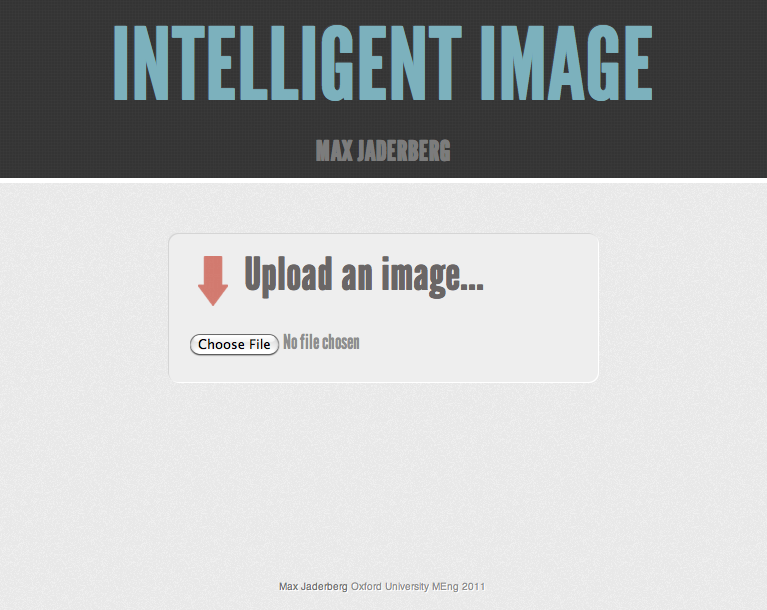
\includegraphics[width=0.4\textwidth]{images/stage1.png}}
~
\subfloat[Stage 2 -- start matching process]{\label{fig:tagimage}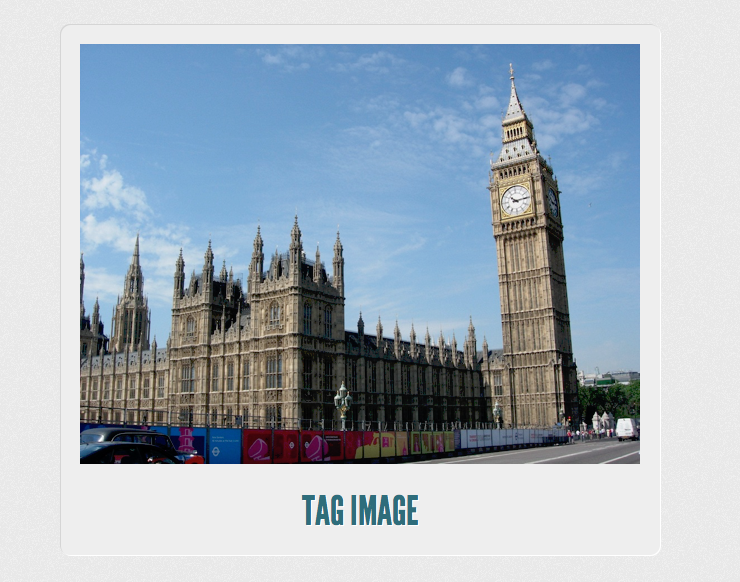
\includegraphics[width=0.4\textwidth]{images/stage2.png}}
\\
\subfloat[Stage 3 -- log of matching process]{\label{fig:log}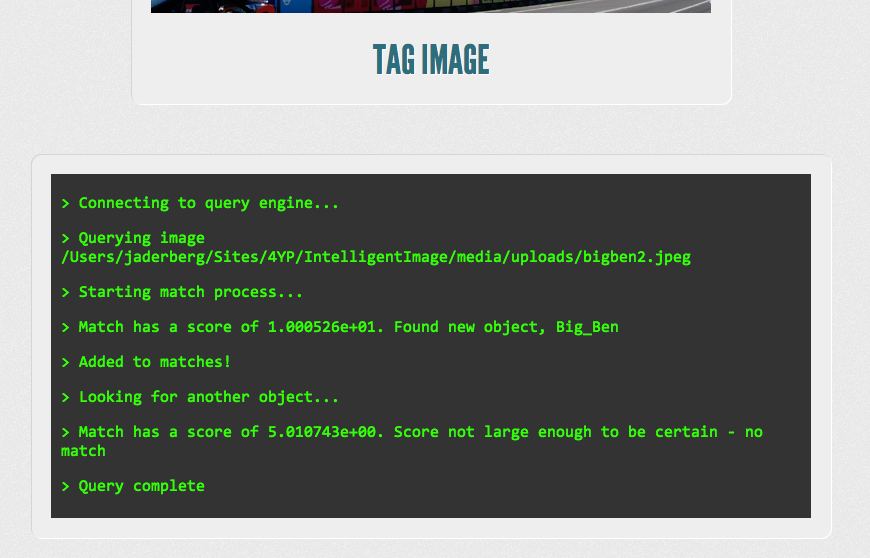
\includegraphics[width=0.4\textwidth]{images/log.png}}
~
\subfloat[Stage 4 -- the intelligent image]{\label{fig:taggedimage}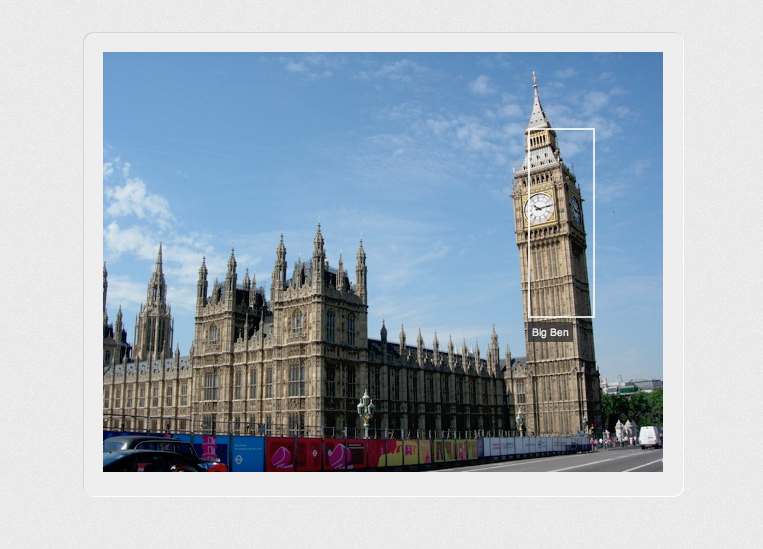
\includegraphics[width=0.4\textwidth]{images/stage3.png}}
\\
\caption{Screenshots showcasing the web application's functionality.}
\label{fig:webapp}
\end{figure}


Figure~\ref{fig:webapp} shows the steps for a user using the website which, are as follows:

\begin{enumerate}
\item Select and upload an image.
\item Click ``Tag Image'' to start the matching process.
\item View the log of the matching process.
\item When match is complete, view and interact with the intelligent image.
\end{enumerate}

\subsection{Front-end}
\label{subsec:front}
The front-end is a web page viewed in a web browser. It consists of three components: the HTML code that defines the structure and layout of the web site, the CSS\footnote{Cascading style sheets -- more information at \url{http://www.w3schools.com/css/}} that defines the styling and the Javascript that provides the logic for the website.

The Javascript scripts make heavy use of the JQuery library\footnote{\url{http://jquery.com}}. JQuery abstracts and simplifies manipulation of HTML elements on the page as well as providing built in animation and HTTP request functions. 

The goal of the website is to appear smooth and responsive, therefore all requests after the initial loading of the page are done asynchronously. This means that Javascript handles all subsequent HTTP requests and responses in the background, without refreshing the browser state. This is done using JQuery's \lstinline!getJSON()! function, where the response data is packaged in JSON format.

\lstset{language=HTML}
The website consists of the four stages described above, and there is an HTML  \lstinline!div! (a container element) for each stage. The CSS styles these to look indented in the page to provide a point of focus for the user. The four containers for each stage are all included in the initial HTML. However, only the stage that is currently active is shown by adding the following attribute to the other containers: \lstinline!style="display: none;"!. 

Initially, the user is presented with an image upload form (see Figure~\ref{fig:uploadform}). Once an image has been selected, a Javascript event is fired, prompting the automatic asynchronous upload of the image. The server responds with HTML to display the image which is inserted in the next container and shown (Figure~\ref{fig:tagimage}).

Upon clicking the ``Tag Image'' button, the real-time log is displaying informing the user of the progress of the matching process (Figure~\ref{fig:log}). The real-time log is achieved by the MATLAB process writing a log file and the Javascript app periodically asking the web server for the contents of the latest version of that file.

Once the match process is complete, the intelligent image HTML (shown in Listing~\ref{lst:intimage}) is returned to the Javascript app. The image is shown with the tags for the objects overlaid. On hover over, the border of the tag becomes solid and the name of the object is shown (Figure~\ref{fig:taggedimage}). On click, the Wikipedia page for the object is opened. This is achieved purely with HTML and CSS.

\linespread{1} % single line spacing
\lstset{language=HTML,caption=The HTML code for the intelligent image.,label=lst:intimage}
\begin{lstlisting}[frame=single]
<!--HTML-->
<div class="tagged-img-wrap">
	<img id="tagged-img" src="/uploads/query_image.jpg}">
	<a style="left: 105px; bottom: 232px;" class="img-tag" href="http://en.wikipedia.org/wiki/Tower_Bridge}" target="_blank">
		<div style="width: 303px; height:288px;" class="tag-border"></div>
		<span class="tag-label">Tower Bridge</span>
        </a>
</div>
\end{lstlisting}
\linespread{2} % double line spacing

\subsection{Back-end}
\label{subsec:back}
The back-end web server is in place to handle all incoming HTTP requests and produce appropriate responses. 

In this application, a Python web server using the Django framework\footnote{Django is an open source web framework written in Python. See \url{https://www.djangoproject.com}.} is used. The HTTP requests are routed to different Python functions depending on what URL is requested, and these functions handle the processing of the request and the rendering of a response. All responses are in JSON format except for the response for the home page which is HTML.

The Django application uses a MySQL database to store user session data as well as the references and details of uploaded images. To perform a matching process, the Django application uses the Python-MATLAB bridge described in Section~\ref{sec:bridge} to start the job and receive the results for subsequent rendering.

\section{Python-MATLAB Bridge}
\label{sec:bridge}
The object recognition engine runs in MATLAB, however the web application runs in Python. Therefore a bridge between the two environments is needed for interaction. In essence, Python code needs to be able to call a MATLAB function and interpret the result.

Some solutions already exist for this purpose\footnote{See \url{http://claymore.engineer.gvsu.edu/~steriana/Python/pymat.html} for an example.} however these all involve starting an instance of MATLAB for each function call. As the system should be fast and scalable, this is not a desirable solution, as there will be a 5-10 second overhead for each MATLAB function call while MATLAB starts up.

\lstset{language=Matlab}
Instead, a Python-MATLAB bridge was developed using MATLAB's Java runtime environment. This is open source and available from \cite{pymatbridge}. Using some code written by D. Kroon (University of Twente), Java's TCP and socket libraries are used to create a TCP server to handle requests. This is run on a separate TCP port to the web application to avoid cross communication. This means that MATLAB needs to startup only once, after which function calls are issued with local HTTP requests. For example, to call the function \lstinline!test_connect()! in the file \lstinline!test_connect.m! with the MATLAB server running on port \lstinline!4000!, simply issue an HTTP request to \lstinline!http://localhost:4000/test_connect.m!. Arguments to the function can be added as query parameters to the HTTP request and decoded by the MATLAB function.

A MATLAB function \lstinline!web_feval! with a supporting function \lstinline!run_dot_m! simplifies this process so any MATLAB function can be called (whether it be on MATLAB's path or not) with any number of arguments, with the results returned as JSON structures. A Python class \lstinline!Matlab! abstracts this on the Python side -- any locally stored MATLAB function can be run, with arguments, and the results are returned as a Python dictionary. Listing~\ref{lst:pymat} shows how a MATLAB function is called with the created class. The \lstinline!run()! function takes two arguments: the location of the function and a dictionary of arguments to be passed in to the function.
 
\linespread{1} % single line spacing
\lstset{language=Python,caption=Python code to run the object matching MATLAB function.,label=lst:pymat}
\begin{lstlisting}[frame=single]
## Python
# First initialise the Matlab object. This is done once when the web server starts
matlab = Matlab('http://localhost:4000')
# Now run the desired function
while matlab.running:
	# Matlab is already processing something, wait
        time.sleep(2)
resp = matlab.run('~/Sites/4YP/visualindex/wikilist_dataset/demo_wiki_get_objects.m', {'image_path': query_image_path, 'display': 1, 'log_file': '%slogs/%s-log.txt' % (settings.MEDIA_ROOT, request.POST.get('key'))}, maxtime=999999)
# Get the results
result = resp['result']
\end{lstlisting}
\linespread{2} % double line spacing

With this bridge, running any MATLAB function becomes trivial and so the web application can run the MATLAB matching process.

\section{Examples}

Figure~\ref{fig:anotations} shows various example results and a video of the implemented system can be found at \cite{video}.

\begin{figure}[htb]
\centering 
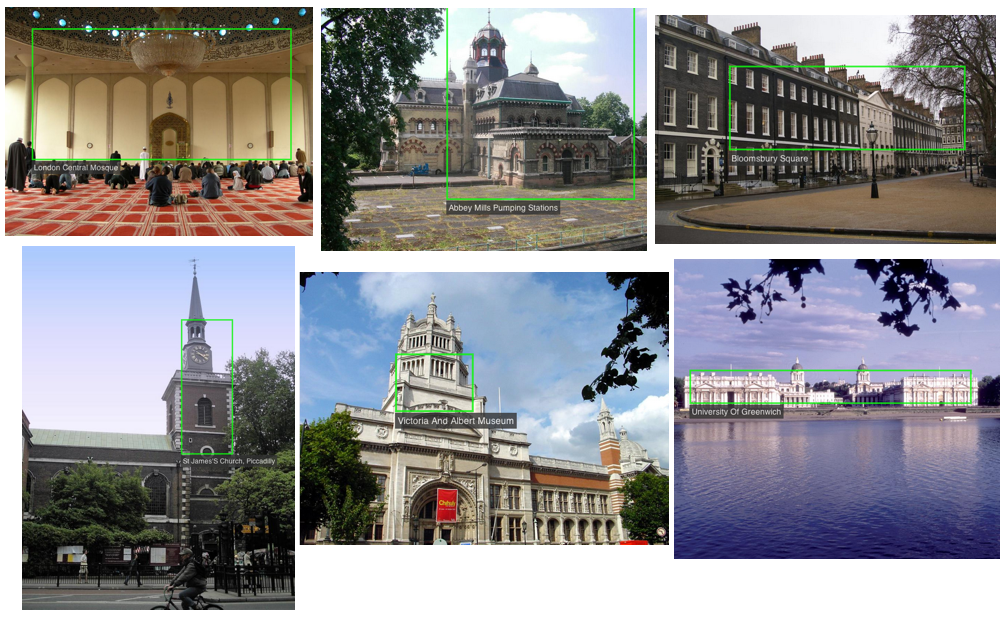
\includegraphics[width=1.0\textwidth]{images/anotatedimages}
\caption{A selection of annotated images. Clockwise from top left: London Central Mosque, Abbey Mills Pumping Station, Bloomsbury Square, University of Greenwich, Victoria and Albert Museum, and St Jame's Church, Piccadilly.}
\label{fig:anotations}
\end{figure}


%-------------------------------
% Summary
%-------------------------------
\linespread{1}\chapter{Summary}
This project aimed to perform large scale image retrieval to provide automatic object recognition to images. The object classes were taken from Wikipedia, and for the purpose of this project, a subset of objects ``Structures in London'' was used for development and testing.

The image data for the model was crawled from Wikipedia, while the turbo-boosting images and test images were gathered from Bing and Google respectively.  

A baseline system was built to incorporate all the functionality desired. The resulting MATLAB object recognition engine can recognise and tag multiple objects in a single image using the Wikipedia data, and this communicates with a Python web application to allow users to interact with the system over the internet. The performance achieved by this baseline system was a yield of 18.1\%, leaving a lot of room for improvements.

A number of extensions to the baseline system were researched and implemented to improve the performance. Alternative geometric models were explored such as NOSAC, and an affine invariant feature detector was used. In conjunction with mapping the feature descriptors from SIFT space to RootSIFT space, these improvements helped increase the recognition performance by a maximum of 35\% compared to the baseline system, to a yield of 24.5\%.

A novel method was developed called turbo-boosting to further build upon the baseline system in an independent way to the geometric improvements. The turbo-boosting process augments the model images with images gathered from Microsoft's Bing. The turbo-boosting, combined with the geometric improvements, dramatically increases the performance of the system -- recognition increased by 75\% compared to the baseline system, giving a yield of 31.7\%.

The results of the project show that a user friendly object tagging website can be built with a maximum yield performance achieved of 31.7\%. This is good, but still leaves many objects unrecognised. The images that were not able to be recognised are generally where the image shows a very different viewpoint, or focuses on a different aspect of the object, which does not appear in the database of model images. This is to be expected, as the dataset used to create the database, the images from Wikipedia, is very noisy and sparse when it comes to representative images. Images from Wikipedia may only contain one or two images of an object, and so do not cover the range of views that, for example, an inquisitive tourist may capture. While methods like turbo-boosting help in bolstering the Wikipedia dataset, the overall lack of representative ground-truth images is thought to be the main limiting factor.

Further work would aim to increase the yield and scale the size of the database. For the yield, better filtering of the Wikipedia dataset could be done, as well as the removal of distracting features that do not uniquely define a class \cite{turcot09}. The textual content of Wikipedia articles could also be harnessed, together with the articles' images, to find more ground-truth images to represent objects. Also a general class representation of the model images could be created, so that initial matching is done on a class level, and subsequently on an image level, thus reducing the amount of in memory data required. The labelling of objects could also be done in a more probabilistic way -- instead of simply defining the object found by the class of the first image that is spatially verified, use some algorithm to determine the most likely object given the top spatially verified images, with some uncertainty score.

%-------------------------------
% References
%-------------------------------
\begin{thebibliography}{99}

	\bibitem{quack09}
		T. Quack, L. Bossard, S. Gammeter and L. Van Gool.
		I know what you did last summer: object-level auto-annotation of holiday snaps.
		In \emph{ICCV}, 2009.

	\bibitem{turcot09}
		P. Turcot and D. G. Lowe.
		Better matching with fewer features: The selection of useful features in large database recognition problems.
		In \emph{WS-LAVD, ICCV}, 2009.
		
	\bibitem{randomforest2}
		C. Silpa-Anan and R. Hartley.
		Localization using an image-map.
		In \emph{Proc. ACRA}, 2004.
		
	\bibitem{rootsift12}
		R. Arandjelovi\'{c} and A. Zisserman.
		Three things everyone should know to improve object retrieval.  
		In \emph{IEEE Conference on Computer Vision and Pattern Recognition}, 2012.
		
	\bibitem{searchengines2003}
		Y. Aashcim, M.Lida, and K. Risvik.
		Multi-tier architecture for web search engines.
		In \emph{Proc. Web Congress}, 2003.
		
	\bibitem{googlearchitecture2003}
		L. Barroso, J. Dean and U. Holzic.
		Web search for a planet: The google cluster architecture.
		In \emph{Micro, IEEE, 23}, 2003.
		
	\bibitem{recognitiontree2006}
		D. Nist\'{e}r and H. Stew\'{e}nius.
		Scalable recognition with a vocabulary tree.
		In \emph{Proc. CVPR}, 2006.
	
	\bibitem{randomforest1}
		Y. Amit and D. Geman. 
		Shape quantization and recognition with randomized trees. 
		In \emph{Neural Computing, 9(7):1545�1588}, 1997.
	
	\bibitem{videogoogle2003}
		J. Sivic and A. Zisserman.
		Video Google: A text retrieval approach to object matching in videos.
		In \emph{Proc. ICCV}, 2003.
		
	\bibitem{lowe1999}
		D. Lowe.
		Object recognition from local scale-invariant features. 
		In \emph{Proc. CVPR}, 1999.
	 
	\bibitem{philbin2007}
		J. Philbin, O. Chum, M. Isard, J. Sivic, and A. Zisserman. 
		Object
retrieval with large vocabularies and fast spatial matching. 
		In \emph{Proc. CVPR}, 2007.
		
	\bibitem{hierarchies2006}
		K. Mikolajczyk, B. Leibe, and B. Schincle.
		Multiple object class detection with a generative model.
		In \emph{Proc. CVPR}, 2006.
	  
	\bibitem{randomforest2005}
		V. Lepetit, P. Lagger, and P.Fua.
		Randomized trees for realtime keypoint recognition.
		In \emph{Proc. CVPR}, 2005.
	 
	 \bibitem{zisserman2004}
	 	R. I. Hartley and A. Zisserman.
		\emph{Multiple View Geometry in Computer Vision.}
		Cambridge University PRess, ISBN: 0521540518, second edition, 2004.
		
	\bibitem{sceneclass06}
		A. Bosch, A. Zisserman and X. Munoz.
		Scene classification via pLSA.
		In \emph{European Conference on Computer Vision}, 2006.
		
	\bibitem{knopp10}
		J. Knopp, J. Sivic and T. Pajdla.
		Avoiding confusing features in place recognition.
		In \emph{European Conference on Computer Vision}, 2010.
		
	\bibitem{quack08}
		T. Quack, B. Leibe and L. Van Gool.
		World-scale Mining of Objects and Events from Community Photo Collections.
		In \emph{CIVR}, 2008.
		
	\bibitem{pymatbridge}
		\url{https://github.com/jaderberg/python-matlab-bridge}
		
	\bibitem{wikipedia}
		\url{http://en.wikipedia.org}
		
	\bibitem{listofstructures}
		\url{http://en.wikipedia.org/wiki/List_of_structures_in_London}
		
	\bibitem{video}
		\url{http://www.youtube.com/watch?v=NFFOjgw7QhM}
		
	\bibitem{listofstructurespdf}
		\url{https://www.dropbox.com/s/lbdcjd58bs1rmot/List%20of%20structures%20in%20London.pdf}
	  
\end{thebibliography}

\end{document}